%%% main.tex — ICE-UTxO: Interleaving Coroutine Effects for Proof-Carrying UTxO Transactions
\documentclass[11pt,a4paper]{article}
\usepackage[margin=1in]{geometry}
\usepackage{hyperref}
\usepackage{xcolor}

%%% ── Packages ──────────────────────────────────────────────────────────────
\usepackage{amsmath}
\usepackage{amssymb}
\usepackage{mathtools}
\usepackage{stmaryrd}
\usepackage{tikz}
\usepackage{listings}
\usepackage{booktabs}
\usepackage{adjustbox}
\usepackage{cleveref}

%%% ── TikZ libraries ───────────────────────────────────────────────────────
\usetikzlibrary{positioning,arrows.meta,shapes,fit,backgrounds,automata,calc,
                 patterns,decorations.pathreplacing}

%%% ── Shared colour palette (Material Design, desaturated for academic use) ──
\definecolor{palBlue}{HTML}{1976D2}
\definecolor{palBlueLt}{HTML}{E3F2FD}
\definecolor{palGreen}{HTML}{388E3C}
\definecolor{palGreenLt}{HTML}{E8F5E9}
\definecolor{palOrange}{HTML}{E65100}
\definecolor{palOrangeLt}{HTML}{FFF3E0}
\definecolor{palPurple}{HTML}{7B1FA2}
\definecolor{palPurpleLt}{HTML}{F3E5F5}
\definecolor{palRed}{HTML}{C62828}
\definecolor{palRedLt}{HTML}{FFEBEE}
\definecolor{palGray}{HTML}{455A64}
\definecolor{palGrayLt}{HTML}{ECEFF1}
\definecolor{palTeal}{HTML}{00796B}
\definecolor{palTealLt}{HTML}{E0F2F1}

%%% ── Shared TikZ styles ─────────────────────────────────────────────────────
\tikzset{
  stdnode/.style={draw, rounded corners, font=\small, minimum height=0.7cm,
                  inner sep=4pt},
  evtnode/.style={stdnode, minimum height=0.7cm, font=\footnotesize},
  fsmstate/.style={draw, rounded corners, minimum width=1.6cm,
                   minimum height=0.7cm, font=\small},
  modnode/.style={draw, rounded corners, minimum width=2.5cm,
                  minimum height=0.7cm, font=\small},
  actornode/.style={draw, rectangle, minimum width=1.4cm,
                    minimum height=0.7cm, font=\small, thick},
  sortbox/.style={draw, minimum width=0.9cm, minimum height=0.7cm,
                  font=\small},
  layernode/.style={draw, rounded corners, minimum width=9cm,
                    minimum height=1.3cm, align=center, font=\small},
  trackgroup/.style={draw, dashed, rounded corners, inner sep=10pt,
                     fill opacity=0.15},
  stdarrow/.style={-{Stealth[length=5pt]}, thick, shorten >=2pt, shorten <=2pt},
  conflictline/.style={dashed, thick, palRed},
  stutterarrow/.style={dotted, thick, -{Stealth[length=4pt]}},
}

%%% ── Theorem environments ────────────────────────────────────────────────
\usepackage{amsthm}
\newtheorem{theorem}{Theorem}[section]
\newtheorem{lemma}[theorem]{Lemma}
\newtheorem{corollary}[theorem]{Corollary}
\newtheorem{proposition}[theorem]{Proposition}
\newtheorem{remark}[theorem]{Remark}
\newtheorem{definition}[theorem]{Definition}

%%% ── Listings setup for Lean 4 ───────────────────────────────────────────
\lstdefinelanguage{Lean4}{
  morekeywords={theorem,lemma,def,structure,inductive,where,let,have,by,
    import,open,namespace,end,if,then,else,match,with,do,return,sorry,
    axiom,instance,class,extends,section,variable,set_option,example},
  sensitive=true,
  morecomment=[l]{--},
  morecomment=[s]{/-}{-/},
  morestring=[b]",
  literate={→}{$\to$}1 {∀}{$\forall$}1 {∃}{$\exists$}1 {¬}{$\neg$}1
           {∈}{$\in$}1 {∧}{$\wedge$}1 {∨}{$\vee$}1 {≤}{$\leq$}1
           {₀}{$_0$}1 {₁}{$_1$}1 {ₙ}{$_n$}1,
}
\lstset{
  language=Lean4,
  basicstyle=\ttfamily\small,
  keywordstyle=\bfseries,
  commentstyle=\itshape\color{gray},
  breaklines=true,
  frame=single,
  xleftmargin=1em,
  numbers=none,
}

%%% ── Convenience macros ──────────────────────────────────────────────────
\newcommand{\NN}{\mathbb{N}}
\newcommand{\Pfin}{\mathcal{P}_{\text{fin}}}
\newcommand{\ie}{i.e.\@\xspace}
\newcommand{\eg}{e.g.\@\xspace}

%%% ── Title and author ────────────────────────────────────────────────────
\title{ICE-UTxO: A Mechanized Conservative Extension of eUTxO\\with Multiparty Session Types}

\author{Charles Hoskinson\\
  \textit{Input Output Group}\\
  \texttt{Charles.Hoskinson@gmail.com}
}

\date{}

\begin{document}
\maketitle

\begin{table}[t]
\caption{Acronyms and abbreviations.}
\label{tab:acronyms}
\centering
\begin{tabular}{ll}
\toprule
\textbf{Acronym} & \textbf{Expansion} \\
\midrule
eUTxO & Extended Unspent Transaction Output \\
ICE & Interleaving Coroutine Effects \\
IVC & Incrementally Verifiable Computation \\
MPST & Multiparty Session Types \\
PCD & Proof-Carrying Data \\
PTB & Programmable Transaction Block \\
S-BAC & Sharded Byzantine Atomic Commit \\
ZK & Zero-Knowledge (proof) \\
\bottomrule
\end{tabular}
\end{table}

\begin{abstract}
Validators in the extended UTxO (eUTxO) model execute once per transaction: they cannot pause, resume, or interact with other on-chain components, leaving multi-step, multi-party coordination without direct ledger support.

We present ICE-UTxO, a conservative extension of eUTxO that adds three layers---coroutine state on UTxOs, coordination scripts expressed as multiparty session type (MPST) global types with event-structure semantics, and Incrementally Verifiable Computation (IVC) proof artifacts that gate commit. When unused, all three layers collapse and ICE-UTxO degenerates to standard eUTxO. Coordination scripts specify permitted interactions as MPST global types; projection extracts per-role local types whose verification can be decomposed across shards.

The model is mechanized in Lean~4 (approximately 4,500~lines, zero \texttt{sorry}, zero custom axioms). The principal results are: strong conflict serializability via a constructive bubble-sort proof establishing that all conflict-respecting permutations of the committed history produce identical core state; concurrent-to-serial refinement via stuttering simulation; bidirectional MPST-to-ledger bridge theorems establishing that shard-local verification of projected traces is necessary and sufficient for global protocol consistency; and a mechanized conservative extension theorem showing that plain eUTxO embeds faithfully into ICE-UTxO. A parallel TLA+ specification validates temporal properties---eventual commit, termination, and effect handling---that Lean's logic cannot express. Cryptographic primitives and the S-BAC consensus layer are modeled as oracles with explicit security assumptions.

To our knowledge, the serializability result is the first machine-checked proof of this property for a UTxO ledger with concurrent interleaving semantics.
\end{abstract}

\noindent\textbf{Keywords:} UTxO, multiparty session types, event structures, formal verification, Lean~4, TLA+, zero-knowledge proofs

\medskip

%% ═══════════════════════════════════════════════════════════════════════════
\section{Introduction}\label{sec:intro}

\begin{quote}
\textbf{Core idea.} A transaction is a proof-carrying implementation of a multiparty protocol; the PTB program is the concrete schedule, and the IVC witness certifies its validity.
\end{quote}

\subsection{The Problem: Transactions as Single-Shot Validators}\label{sec:problem}

In the eUTxO model~\cite{Chakravarty2020}, a transaction consumes inputs, executes validators, and produces outputs. Each validator is a pure function: it receives a datum, a redeemer, and a read-only transaction context, and returns accept or reject. The model suits simple transfers but fails when applications need multi-step coordination across multiple UTxOs within a single atomic transaction.

Developers have converged on three workarounds, none satisfactory. \emph{Transaction chaining} splits workflows across multiple transactions. This loses atomicity: intermediate states become visible on-chain, and any step can fail independently, enabling front-running and race conditions. \emph{Monolithic validators} take the opposite approach, encoding the entire interaction in a single script. This preserves atomicity but loses modularity: the validator becomes a single point of complexity that cannot be composed from independent components. \emph{Off-chain protocols} such as Hydra heads move interactions off-chain entirely, introducing additional trust assumptions and infrastructure requirements. None resolves atomicity, modularity, and verifiability simultaneously.

\paragraph{Multi-step interactions.}
Consider a DeFi protocol in which two UTxOs must interact across several resume/yield cycles within a single atomic transaction. For instance, a collateralized loan liquidation may require: (1)~reading an oracle UTxO for a price feed, (2)~computing a liquidation amount in the borrower's UTxO, (3)~transferring collateral to a liquidator UTxO, and (4)~updating the protocol's global state UTxO---all atomically. The eUTxO validator model has no notion of ``pause and resume''; each validator executes exactly once, sees only its own datum, and cannot carry forward intermediate state.

In current eUTxO practice, a developer would encode this as a monolithic validator that inspects the full transaction context---functional but complex and non-reusable. Splitting into multiple transactions introduces race conditions (the oracle price may change between steps). Ethereum handles this via synchronous contract calls, but its account model sacrifices the parallel validation that UTxOs provide. ICE-UTxO offers an alternative: each component (oracle, borrower, liquidator, protocol state) remains an independent UTxO with its own validator, and the coroutine and effect system coordinates them within a single atomic transaction according to a session-typed protocol.

\paragraph{Cross-contract communication.}
A related limitation arises when two contracts need to exchange data during execution, not just at the transaction boundary. The eUTxO model forces developers into one of two unsatisfying choices: encode the entire multi-contract interaction as a single monolithic validator (sacrificing modularity), or split the interaction across multiple transactions (sacrificing atomicity). Neither preserves both properties.

\paragraph{Effect handling.}
A UTxO frequently needs to request a service (an oracle lookup, a token burn authorization, a permission check) and receive a result before continuing its computation. The validator model provides no mechanism for structured effects: there is no way for a validator to ``raise'' a request, have it handled by some external service within the same transaction, and then ``resume'' with the result.

\paragraph{Proof of coordination.}
Even if one could engineer multi-step interactions through clever datum encoding, there is no standard way to \emph{prove} that the interleaving was valid: that the schedule of operations respected causal dependencies and did not violate protocol invariants. The validity of the coordination is implicit in the validator logic, not an explicit, verifiable artifact.

To ground these limitations concretely, consider a cross-chain DEX aggregator. The system must atomically execute four steps: query an oracle for the current price of asset~A in terms of asset~B, check the user's collateral position against the quoted price, execute a swap on one liquidity pool if the price is favorable, and route to an alternative pool if not. All four must succeed or fail together---partial execution would expose the user's collateral to arbitrage.

In the current eUTxO model, encoding this requires either a monolithic validator that internalizes all routing logic (creating a maintenance burden and limiting composability with third-party pools), or a transaction chain that splits the steps across separate transactions (introducing race conditions where the price may change between steps). State channel approaches like Hydra~\cite{Hydra2023} could handle the interaction off-chain, but only among parties already sharing a Hydra head.

ICE-UTxO offers a third path: each component---oracle, collateral checker, liquidity pools---remains an independent UTxO with its own validator, coordinated by a session-typed protocol whose IVC proof certifies correct execution.

Today's eUTxO validators resemble sequential functions---powerful for their intended scope, but constrained when applications require richer interaction patterns. What is needed is a model where transactions are \emph{concurrent programs with communication}, and where the schedule itself is a \emph{verified artifact}.

\subsection{The Insight: Transactions as Multiparty Protocols}\label{sec:insight}

The central idea is a change of perspective: ICE-UTxO treats each transaction as an instance of a \emph{multiparty session protocol}. In standard eUTxO, a transaction is a batch operation---consume inputs, produce outputs, check validators. ICE-UTxO reframes this as a \emph{conversation}: validators are participants in a protocol, and the transaction is one round of that protocol. A validator can pause (yield control and store its state), request a service (raise an effect), and later resume with the result. The rules governing who acts when are specified as a coordination script. This reframing resolves the limitations above by introducing three interlocking concepts:

\paragraph{UTxO coroutines}
are participants that can yield (pause execution) and resume, carrying their execution state as part of their UTxO datum. Concretely, each coroutine-enabled UTxO stores a \emph{frame}---a tuple of program counter, local variables, method identifier, and a cryptographic hash binding the frame to its execution history (formalized in \cref{def:frame}). The UTxO lifecycle extends from \texttt{Created} through \texttt{Suspended\_at\_Yield} or \texttt{Suspended\_at\_Effect} to \texttt{Consumed} (the full lifecycle state machine is given in \cref{sec:lifecycle}, \cref{fig:lifecycle}). A coroutine that yields produces a new UTxO with an updated frame; a coroutine that is consumed has completed its participation in the transaction.

\paragraph{Effect handlers}
are dynamically-scoped services installed by the coordination script. When a coroutine raises an effect (e.g., ``I need the current ETH/USD price''), the effect propagates to the nearest installed handler for that interface. The handler processes the effect and resumes the coroutine with a result. This is the \emph{algebraic effects} pattern from programming language theory~\cite{PlotkinPretnar2009}, adapted to the blockchain setting. Handlers are installed and uninstalled explicitly via transaction commands, and their lifetimes are bounded by the transaction scope.

\paragraph{Coordination scripts}
are \emph{global types} in the sense of multiparty session types (MPST)~\cite{Honda2016}. They specify the allowed interactions among roles as an \emph{event structure}---a partial order of events augmented with a conflict relation encoding mutual exclusion. The coordination script specifies the protocol; the compiled PTB program linearizes it into a deterministic schedule; the IVC witness certifies conformance.

Each component addresses a distinct concern. MPST global types specify the allowed multi-party coordination patterns, with well-studied safety and progress guarantees. To capture the independence of non-conflicting operations, event structures replace sequential traces with partial-order semantics. These specifications must then become executable: PTB-style compilation produces a concrete, deterministic format amenable to on-chain validation. Finally, IVC/PCD witnesses transform transactions into \emph{proof-carrying artifacts}---each transaction carries a cryptographic certificate of its own validity, verified by an external ZK verifier whose soundness is an explicit assumption of the model (\cref{sec:state-components}).

Several of these constituent ideas have antecedents in both the blockchain and programming languages literatures. Multi-step contract execution on UTXO-like models has been explored by Ergo's multi-stage contracts~\cite{Chepurnoy2019}, which use transaction trees to encode sequential contract logic across multiple UTXO lifetimes, and by Sui's Programmable Transaction Blocks~\cite{Blackshear2023}, which compose multiple object operations within a single atomic transaction. The algebraic effects pattern is well-established in programming language theory~\cite{PlotkinPretnar2009} and has been applied to various computational settings, though not previously to on-chain UTXO validators. Session types for smart contracts were first explored by the Nomos system~\cite{Das2021}, which uses binary (two-party) session types based on linear logic to ensure resource safety in a concurrent contract language; ICE-UTxO extends this direction to multiparty protocols with arbitrarily many roles. Proof-carrying transactions in the blockchain setting were pioneered by ZEXE~\cite{Bowe2018} and deployed in Aleo~\cite{Aleo2021}, where each transaction carries a zero-knowledge proof of correct state transition; ICE-UTxO adapts this pattern to certify multiparty protocol compliance rather than arbitrary computation. The IVC proof mechanism builds on recent advances in folding schemes, particularly Nova~\cite{Kothapalli2022}, which makes incremental proof generation practical. The novelty of ICE-UTxO lies not in any single component but in their systematic integration: the demonstration that coroutines, algebraic effects, multiparty session types, PTB compilation, IVC proofs, and S-BAC compose coherently as a conservative extension of eUTxO, with the entire combination formally verified in Lean~4.

\subsection{The Architecture: Three Layers on eUTxO}\label{sec:architecture}

ICE-UTxO separates concerns into three layers, each addressing an independent verification question. Layer~1 asks: \emph{can this UTxO resume its computation?} Layer~2 asks: \emph{do these operations follow the declared protocol?} Layer~3 asks: \emph{can we trust the execution without replaying it?} This separation allows each layer to be verified independently and composed via narrow interfaces.

\paragraph{Layer~1: Coroutine state on UTxOs.}
Each UTxO optionally carries a \emph{frame} $(pc, \mathit{locals}, \mathit{methodId}, \mathit{hash})$. The frame records the coroutine's suspension point, enabling it to be resumed in a future transaction step. This is the \emph{process layer}---it provides the mechanism for multi-step execution.

\paragraph{Layer~2: Transaction-level coordination.}
Mechanism alone is not enough; we also need a specification of what coordination is allowed. A coordination script (global type) is compiled to a PTB-style program---a sequence of commands with dataflow through temporary result registers $\mathit{Result}(i)$. This is the \emph{protocol layer}---it constrains which interleavings are valid.

\paragraph{Layer~3: IVC proof artifacts.}
Given mechanism (Layer~1) and specification (Layer~2), the remaining question is trust: how does the ledger verify that the mechanism followed the specification? The transaction carries proof commitments that certify the interleaving trace conforms to the coordination script. Validators check the proof rather than re-execute the coroutine logic. This is the \emph{verification layer}.

\paragraph{Conservative extension.}
When all three layers collapse---no coroutines yield, no effects are raised, no coordination script is needed---ICE-UTxO degenerates to standard eUTxO. Concretely, every standard eUTxO transaction is a valid ICE-UTxO transaction with empty frame fields, no effect handlers, and a trivial coordination witness; the new machinery adds capability without breaking compatibility. The formal statement appears in \cref{sec:reduction}.

\begin{figure}[t]
\centering
\begin{adjustbox}{max width=\linewidth, center}
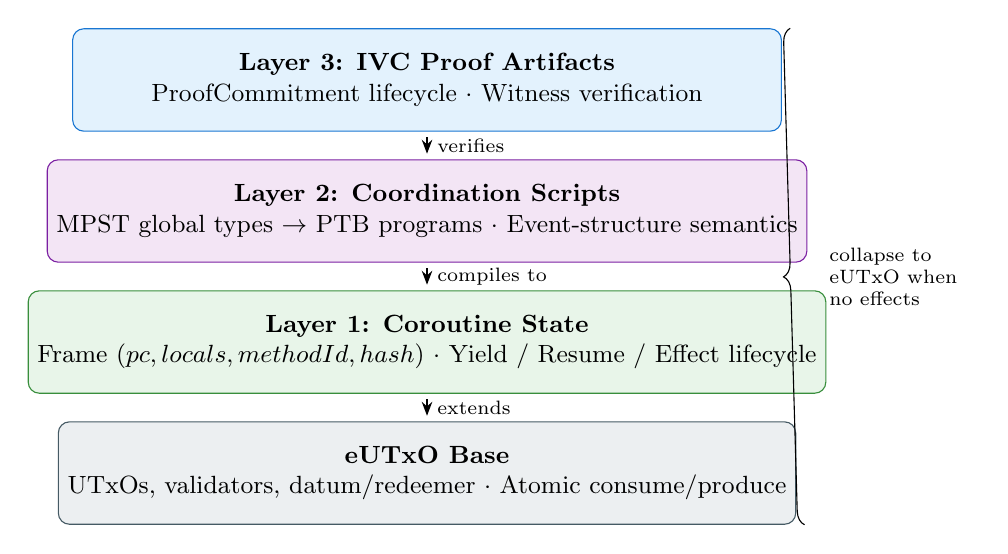
\begin{tikzpicture}[>=Stealth]
%% Nodes
\node[layernode, fill=palBlueLt, draw=palBlue]  (L3) {\textbf{Layer 3: IVC Proof Artifacts}\\ProofCommitment lifecycle $\cdot$ Witness verification};
\node[layernode, fill=palPurpleLt, draw=palPurple, below=0.35cm of L3] (L2) {\textbf{Layer 2: Coordination Scripts}\\MPST global types $\to$ PTB programs $\cdot$ Event-structure semantics};
\node[layernode, fill=palGreenLt, draw=palGreen, below=0.35cm of L2]  (L1) {\textbf{Layer 1: Coroutine State}\\Frame $(pc, locals, methodId, hash)$ $\cdot$ Yield / Resume / Effect lifecycle};
\node[layernode, fill=palGrayLt, draw=palGray, below=0.35cm of L1]   (L0) {\textbf{eUTxO Base}\\UTxOs, validators, datum/redeemer $\cdot$ Atomic consume/produce};
%% Edges
\draw[stdarrow] (L3) -- node[right, font=\scriptsize] {verifies} (L2);
\draw[stdarrow] (L2) -- node[right, font=\scriptsize] {compiles to} (L1);
\draw[stdarrow] (L1) -- node[right, font=\scriptsize] {extends} (L0);
%% Annotation
\draw[decorate, decoration={brace, amplitude=5pt, mirror}]
  ([xshift=3pt]L3.north east) -- ([xshift=3pt]L0.south east)
  node[midway, right=8pt, font=\scriptsize, align=left, text width=1.8cm]
  {collapse to eUTxO when no effects};
\end{tikzpicture}
\end{adjustbox}
\caption{Architecture layers of ICE-UTxO. Layer~1 (coroutine state) extends UTxOs with frames; Layer~2 (coordination) compiles MPST global types to PTB programs; Layer~3 (verification) attaches IVC proof artifacts. When no coroutines yield and no effects are raised, all three layers collapse and ICE-UTxO degenerates to standard eUTxO.}
\label{fig:architecture}
\end{figure}

\subsection{Scope and Non-Goals}\label{sec:scope}

This paper addresses the formal model and its mechanized safety proofs. The following are explicitly out of scope: implementation performance and benchmarking; ZK circuit design and concrete proving systems; developer tooling and language design; incentive-compatibility and mechanism design; and production deployment architecture including cross-shard coordination. Bridge architecture and cross-shard coordination via S-BAC are addressed in a companion paper~\cite{PaperB}.

\subsection{Deployment Model: S-BAC for Cross-Shard Atomicity}\label{sec:deployment}

When a transaction touches only \emph{owned objects} (coroutine frames belonging to a single party), it can proceed on a fast path without full consensus. When it touches \emph{shared objects} (effect handlers, shared state across shards), it requires consensus for atomic commit. ICE-UTxO adopts the Sharded Byzantine Atomic Commit (S-BAC) protocol from Chainspace~\cite{AlBassam2018}:

\begin{itemize}
  \item Each shard checks its \emph{local projection} of the coordination script during the prepare phase.
  \item The IVC witness lets shards validate the interleaving without re-executing private computation.
  \item If all shards prepare successfully, the transaction commits; if any shard aborts, all abort.
\end{itemize}

\begin{table}[t]
\caption{Mapping from Chainspace to ICE-UTxO.}
\label{tab:chainspace-mapping}
\centering
\begin{tabular}{ll}
\toprule
\textbf{Chainspace} & \textbf{ICE-UTxO} \\
\midrule
Object & Frame-carrying UTxO \\
Procedure bundle & PTB program + IVC witness \\
Checker & Witness verifier + ledger checks \\
S-BAC & Cross-shard atomic commit \\
\bottomrule
\end{tabular}
\end{table}

\subsection{Formal Verification: Zero Sorry, Zero Axioms}\label{sec:verification-intro}

The ICE-UTxO ledger-level semantics have been formalized in Lean~4 in about 4,500 lines of code across eleven source files (including \texttt{test\_axioms.lean}) plus \texttt{lakefile.lean}, organized in four core modules (\texttt{StarstreamPilot.lean}, \texttt{Script.lean}, \texttt{PTB.lean}, \texttt{SBAC.lean}) and supporting oracle modules. Cryptographic primitives and the S-BAC consensus layer are modeled as oracles with explicit assumptions (\cref{sec:state-components}). The mechanization achieves:

\begin{itemize}
  \item \textbf{Zero sorry}: no admitted lemmas anywhere in the development.
  \item \textbf{Zero custom axioms}: only the standard Lean kernel axioms (\texttt{propext}, \texttt{Quot.sound}, \texttt{funext}).
  \item \textbf{Minimal classical reasoning}: \texttt{Classical.choice} is never invoked, and the development uses a single localized \texttt{classical} case split; the proofs are otherwise constructive.
\end{itemize}

\subsection{Contributions}\label{sec:contributions}

This paper makes the following contributions:

\begin{enumerate}
  \item \textbf{ICE-UTxO model.} A conservative extension of eUTxO with coroutines, algebraic effects, and proof-carrying transactions (\cref{sec:model,sec:opsem}).
  \item \textbf{Coordination scripts.} A formal language for multiparty coordination based on MPST global types with event-structure semantics (\cref{sec:model}).
  \item \textbf{PTB compilation.} Translation from coordination scripts to PTB-style bytecode---adapting Sui's Programmable Transaction Block format~\cite{Blackshear2023}---with explicit dataflow and formal correctness guarantees (\cref{sec:model}).
  \item \textbf{S-BAC integration.} Shard-local verification using projected coordination scripts, composing Chainspace's S-BAC protocol~\cite{AlBassam2018} with session-type witnesses to enable protocol-aware cross-shard atomic commit (\cref{sec:model,sec:bridge}).
  \item \textbf{Lean~4 mechanization.} Complete formal verification with zero sorry, zero custom axioms, and mostly constructive proofs (\cref{sec:mechanization}).
  \item \textbf{Strong serializability proof.} A constructive bubble-sort proof that acyclic full-conflict precedence graphs imply all conflict-respecting permutations produce the same core state (\cref{sec:serializability}).
  \item \textbf{Systematic integration.} A demonstration that coroutines, algebraic effects, MPST, PTB compilation, IVC proofs, and S-BAC compose coherently as a conservative extension of eUTxO, with the combination verified end-to-end. Individual components draw on established techniques (\cref{tab:novelty} in \cref{sec:related}); the contribution is their integration within a single formally verified framework.
\end{enumerate}

\noindent The contributions are formal: we establish the model and prove its safety properties via mechanized proof. Empirical evaluation of proving costs, transaction throughput, and validation latency under realistic workloads is orthogonal and left to implementation work.

\subsection{How to Read This Paper}\label{sec:howtoread}

This paper serves multiple audiences with different interests. The following guide maps reader backgrounds to relevant sections.

\textbf{For blockchain developers}: \cref{sec:intro,sec:state-components,sec:global-types,sec:projection,sec:lifecycle,sec:commit-rule,sec:concurrency-modes} introduce the model and its operational behavior.

\textbf{For formal methods researchers}: \cref{sec:event-structure-semantics,sec:serializability,sec:bridge} contain the main theoretical contributions. \Cref{sec:mechanization} documents the Lean mechanization.

\textbf{For protocol designers}: \cref{sec:sbac-integration,sec:commit-rule,sec:coordination-witness} describe the deployment architecture and its trust boundaries.

\subsection{Paper Roadmap}\label{sec:roadmap}

\Cref{sec:background} reviews background. \Cref{sec:model} presents the ICE-UTxO model in full. \Cref{sec:opsem} defines the operational semantics and proves ledger safety invariants. \Cref{sec:serializability} establishes strong conflict serializability. \Cref{sec:bridge} bridges the MPST coordination layer to the ledger commit mechanism. \Cref{sec:mechanization} discusses the Lean~4 mechanization. \Cref{sec:related} surveys related work. \Cref{sec:discussion} discusses limitations and future directions. \Cref{sec:conclusion} concludes.

%% ═══════════════════════════════════════════════════════════════════════════
\section{Background}\label{sec:background}

ICE-UTxO combines five ideas from different research communities: the eUTxO ledger model provides the state substrate; multiparty session types specify coordination protocols; event structures give those protocols a partial-order semantics; Programmable Transaction Blocks supply a deterministic execution format; and Sharded Byzantine Atomic Commit handles cross-shard consistency. Each addresses a distinct concern; none suffices alone. The following subsections review each foundation in turn.

\subsection{Extended UTxO}\label{sec:eutxo}

Bitcoin's original UTxO model represents value as \emph{unspent transaction outputs}: discrete ``coins'' that are created by one transaction and consumed by another. Spending a UTxO requires providing a witness (typically a digital signature) that satisfies the locking script attached to that output. While elegant and naturally parallelizable---distinct UTxOs can be validated independently---the original model is limited in expressiveness: there is no persistent state beyond the locked value itself, and the scripting language (Bitcoin Script) is intentionally non--Turing-complete. These constraints make it difficult to encode smart contracts that maintain state across interactions, perform rich computation, or coordinate multiple parties. The \emph{extended UTxO} (eUTxO) model~\cite{Chakravarty2020} was designed to bring smart contract capability to UTxO-based blockchains while preserving the parallelism and deterministic validation that make the UTxO approach attractive. By contrast, Ethereum's account model maintains global mutable state that contracts read and write during execution, enabling rich programmability but introducing sequential execution dependencies, reentrancy vulnerabilities, and non-deterministic gas consumption.

The eUTxO model augments each UTxO with a typed \emph{datum} (persistent state) and each spending transaction with a \emph{redeemer} (an argument provided by the party constructing the transaction). Each \emph{validator} functions as a pure deterministic gate:
\[
\mathit{validator} : \mathit{Datum} \times \mathit{Redeemer} \times \mathit{TxContext} \to \mathit{Bool}
\]
where $\mathit{TxContext}$ provides a read-only view of the transaction's inputs, outputs, validity interval, fee structure, minting policies, and other metadata. Validators are pure functions: given the same datum, redeemer, and context, they always return the same Boolean. This purity enables predictable validation---transaction outcomes can be predicted off-chain before submission, validators can be executed in parallel across distinct UTxOs, and formal verification of validator logic is tractable. Cardano implements eUTxO with Plutus validators, where datums and redeemers are serialized as a universal data type and validators are compiled to Plutus Core (a variant of System~F).

Despite these strengths, the original eUTxO model has limitations. The result: atomicity without modularity, or modularity without atomicity. The most significant limitation is the ``consume to read'' problem: inspecting a UTxO's datum requires including it as a transaction input, which \emph{consumes} it. This forces contention---if two transactions need to read the same datum (e.g., an oracle price feed), they must compete for the UTxO, serializing access. A related issue is the \emph{double satisfaction} problem~\cite{Chakravarty2020}: when a transaction has multiple script inputs, a single output may inadvertently satisfy the validation conditions of two different validators, allowing one validator's intended output to be ``stolen'' by another. Furthermore, multi-step interactions between parties require multiple on-chain transactions across multiple blocks, breaking atomicity and exposing intermediate states to front-running or abandonment.

Several Cardano Improvement Proposals have partially addressed these limitations. CIP-31~\cite{CIP31} introduces \emph{reference inputs}, allowing a transaction to read a UTxO's datum without consuming it---solving the consume-to-read problem for oracle feeds and shared configuration data. CIP-32 introduces \emph{inline datums}, storing data directly in the UTxO output rather than as a hash, reducing the need for off-chain datum management. CIP-33 introduces \emph{reference scripts}, enabling transactions to reference validator scripts stored on-chain rather than re-attaching them to every transaction, significantly reducing transaction size. Together (deployed in the Vasil hard fork), these extensions improve usability and reduce contention, but they still cannot express multi-step atomic protocols---sequences of dependent operations that must all succeed or all fail---within a single transaction.

Other UTxO-based platforms have explored related extensions. Ergo~\cite{Ergo2019} supports \emph{data inputs} (analogous to CIP-31 reference inputs) from its inception and enables multi-stage contracts via ErgoScript, a language based on Sigma protocols that supports non-interactive zero-knowledge proofs natively. Bartoletti and Zunino's BitML~\cite{Bartoletti2018} provides a process calculus for Bitcoin smart contracts with formal compilation to standard Bitcoin transactions, demonstrating that surprisingly rich contract logic can be encoded even in Bitcoin's restricted scripting model. More recently, proposals for Bitcoin \emph{covenants}---notably BIP-119 (OP\_CHECKTEMPLATEVERIFY)---would allow a UTxO's spending conditions to constrain the \emph{outputs} of the spending transaction, propagating conditions forward in the UTxO graph. Vinogradova and Melkonian~\cite{Vinogradova2024} explore message-passing semantics for eUTxO, providing a communication-oriented perspective on inter-UTxO interaction. ICE-UTxO builds on the post-Vasil eUTxO model and extends it further with coroutines and algebraic effects, enabling multi-step atomic protocols within a single transaction while retaining the deterministic, parallelizable character of UTxO validation.

\subsection{Multiparty Session Types}\label{sec:mpst-bg}

The eUTxO extensions above enable richer computation within individual UTxOs, but they do not provide a formal coordination language for multi-party interactions. Session types fill this gap. They specify communication protocols among multiple parties, with mechanical safety guarantees: a well-typed protocol cannot deadlock, and no participant can send the wrong message at the wrong time. They function as typed contracts for message exchange, analogous to function type signatures that prevent calling a function with incorrect argument types. Originally developed for binary (two-party) sessions by Honda et al., the theory was extended to the multiparty setting (MPST) by Honda, Yoshida, and Carbone~\cite{Honda2016}, enabling protocols involving three or more roles with complex interaction patterns including delegation, branching, and recursion. The MPST framework has since been applied to verify communication-intensive systems including web services, operating system kernels, and distributed algorithms~\cite{Huttel2016}.

A \emph{global type}~$G$ specifies the complete protocol from an omniscient perspective. For instance, if role~$p$ sends a price request to role~$q$, who then responds with a price, the global type records both steps in sequence. The formal syntax captures this as a grammar:
\[
G ::= p \to q : \langle S \rangle . G \mid G_1 + G_2 \mid \mu X . G \mid X \mid \mathbf{end}
\]
The constructor $p \to q : \langle S \rangle . G$ means that role~$p$ sends a message of payload type~$S$ to role~$q$, after which the protocol continues as~$G$. The choice $G_1 + G_2$ represents a branching point where the protocol may proceed along either branch (typically determined by a designated role). The recursion $\mu X . G$ binds the variable~$X$ in~$G$, enabling repeating protocols such as auction rounds or heartbeat exchanges; $\mathbf{end}$ terminates the session. \emph{Projection} extracts a \emph{local type} $L_r = G \upharpoonright r$ for each role~$r$, describing only that role's own sends and receives. If every participant faithfully follows its projected local type, the global protocol specification is satisfied.

The MPST metatheory establishes three key safety properties~\cite{Bettini2008,Coppo2013,Scalas2016}. \emph{Communication safety} ensures that no type mismatch can occur: when a role sends a message of type~$S$, the receiving role expects exactly type~$S$. \emph{Protocol conformance} guarantees that each party's runtime behaviour is an instance of its projected local type---no party can deviate from the prescribed interaction sequence. \emph{Progress} (deadlock-freedom) ensures that well-typed sessions always advance: no configuration arises where every role is waiting for a message that will never be sent. Progress typically requires well-formedness conditions on the global type (e.g., no mixed choices where different roles independently decide different branches) and fairness assumptions (messages are eventually delivered).

In ICE-UTxO, session types are applied in a setting that differs fundamentally from the traditional distributed-processes-over-channels model. Sessions are scoped to a single atomic transaction: all protocol steps occur within one transaction, not across multiple blocks or network round-trips. This has a simplifying consequence for progress---because a transaction either executes completely or not at all (atomicity), ``message delivery'' is guaranteed within the session scope, and progress reduces to an all-or-nothing property rather than requiring ongoing fairness. Each UTxO participating in the protocol plays a role in the session; its validator enforces the projected local type by checking that the transaction's structure matches the expected communication pattern. Adversarial deviation---a participant attempting to execute a transaction that violates the protocol---is prevented by proof-carrying semantics (\cref{sec:model}): each transaction carries cryptographic evidence that the executed schedule conforms to the coordination script.

The MPST framework has been extended in numerous directions: asynchronous communication with bounded buffers~\cite{Scalas2016}, timed sessions with deadline constraints, session delegation (passing a session endpoint to another party), and session subtyping. Of particular relevance to ICE-UTxO is the event-structure semantics for MPST developed by Castellani et al.~\cite{Castellani2023}, which interprets global types not as sequential traces but as event structures (\cref{sec:event-structures-bg}). This interpretation captures the \emph{concurrency} inherent in multiparty protocols: when two communication actions involve disjoint sets of roles, they are genuinely independent events rather than arbitrarily interleaved sequential steps. ICE-UTxO builds directly on this event-structure semantics to derive correct-by-construction schedules for multi-UTxO coordination.

\subsection{Event Structures}\label{sec:event-structures-bg}

MPST global types specify \emph{what} interactions are allowed, but not \emph{how concurrent} those interactions are---whether two protocol steps must happen sequentially or can occur in any order. Event structures answer this question. Blockchain transactions involving multiple UTxOs often contain operations that are \emph{causally dependent}---one must complete before another can begin (e.g., reading an oracle price before computing a liquidation amount)---as well as operations that are genuinely \emph{independent} (e.g., two unrelated token transfers within the same transaction). A simple sequential model does not capture this distinction: it imposes a total order where none is required, obscuring which operations can be safely reordered. Event structures, introduced by Winskel~\cite{Winskel1986}, provide a mathematical framework that models both causal order and mutual exclusion (\emph{conflict}) explicitly, enabling precise reasoning about concurrency. This is critical for ICE-UTxO's serializability results: by tracking which operations are independent, we can prove that different valid execution orders produce the same outcome.

Formally, an \emph{event structure} is a triple $(E, \leq, \#)$ where $E$ is a set of events, $\leq \subseteq E \times E$ is a partial order representing \emph{causality} (if $e_1 \leq e_2$, then $e_1$ must occur before $e_2$), and $\# \subseteq E \times E$ is a symmetric, irreflexive \emph{conflict} relation, subject to \emph{hereditary conflict}: if $e_1 \mathrel{\#} e_2$ and $e_2 \leq e_3$, then $e_1 \mathrel{\#} e_3$ (conflict propagates forward along causality). A \emph{configuration} $C \subseteq E$ is a set of events that is conflict-free ($\neg(e_1 \mathrel{\#} e_2)$ for all $e_1, e_2 \in C$) and down-closed (if $e \in C$ and $e' \leq e$, then $e' \in C$). Intuitively, a configuration represents a consistent snapshot of ``what has happened so far''---every event's prerequisites are present, and no two mutually exclusive events have both occurred. An event $e$ is \emph{enabled} in configuration~$C$ if $e \notin C$, all predecessors of $e$ under $\leq$ are in $C$, and $e$ does not conflict with any event in $C$. A \emph{valid trace} is a sequence of events $e_1, e_2, \ldots, e_n$ such that each prefix $\{e_1, \ldots, e_k\}$ forms a configuration---equivalently, a chain of configurations from $\emptyset$ to the final state.

Castellani et al.~\cite{Castellani2023} showed that MPST global types can be interpreted as event structures: each communication action ($p \to q : \langle S \rangle$) becomes an event; causal dependencies arise from the protocol's sequential structure (a send must precede its continuation); and conflict arises from choice (the two branches of $G_1 + G_2$ are in conflict, since only one branch can be taken). This gives MPST a \emph{concurrency semantics} rather than an interleaving semantics. The distinction matters for ICE-UTxO because multiple UTxO operations within one transaction may be genuinely independent---their relative order is irrelevant to the outcome---and the event-structure representation captures this independence explicitly, enabling tighter correctness proofs.

Any acyclic event structure can be \emph{linearized}: its events can be topologically sorted into a total order that respects causality. When two events are \emph{concurrent} (neither causes the other, and they are not in conflict), they may appear in either order in a linearization---and, crucially, the resulting state is the same regardless of order. This \emph{confluence} property is the foundation of the serializability results in \cref{sec:serializability}. The PTB compilation (\cref{sec:ptb-compilation}) performs exactly this linearization, producing a deterministic command sequence from the event structure's partial order, with explicit dataflow through result registers ensuring that causal dependencies are respected.

\Cref{fig:event-dag} illustrates a small event structure arising from a coordination script. Event~$e_1$ (install a handler) causally precedes both $e_2$ (resume coroutine $U_1$) and $e_3$ (resume coroutine $U_2$). Event~$e_2$ causally precedes $e_4$ (raise an effect), which in turn precedes $e_5$ (handle the effect). The dashed line between $e_3$ and $e_4$ denotes conflict: they cannot both appear in the same configuration. This models a protocol where $U_1$ and $U_2$ cannot both be active simultaneously---the coordinator must choose which coroutine to resume, and the unchosen path is excluded from the execution.

\begin{figure}[t]
\centering
\begin{adjustbox}{max width=\linewidth, center}
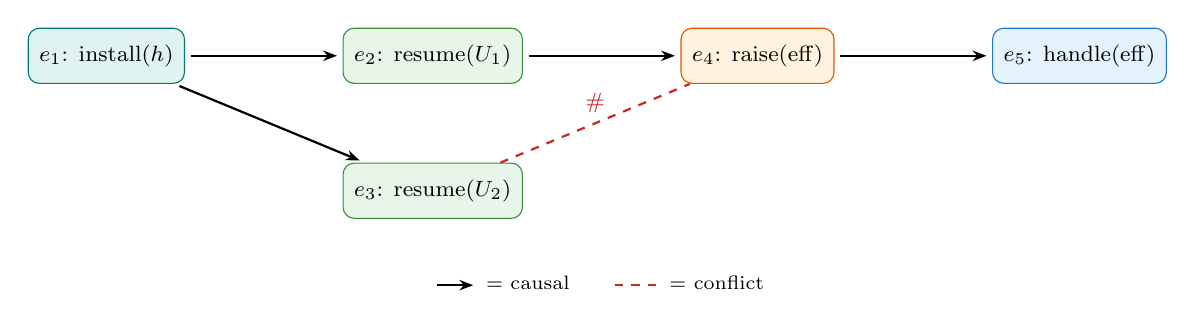
\begin{tikzpicture}[
  node distance=1.5cm and 2.0cm,
  >=Stealth
]
%% Nodes
\node[evtnode, fill=palTealLt, draw=palTeal] (e1) {$e_1$: install$(h)$};
\node[evtnode, fill=palGreenLt, draw=palGreen, right=of e1] (e2) {$e_2$: resume$(U_1)$};
\node[evtnode, fill=palGreenLt, draw=palGreen, below=1.0cm of e2] (e3) {$e_3$: resume$(U_2)$};
\node[evtnode, fill=palOrangeLt, draw=palOrange, right=of e2] (e4) {$e_4$: raise(eff)};
\node[evtnode, fill=palBlueLt, draw=palBlue, right=of e4] (e5) {$e_5$: handle(eff)};
%% Edges
\draw[stdarrow] (e1) -- (e2);
\draw[stdarrow] (e1) -- (e3);
\draw[stdarrow] (e2) -- (e4);
\draw[stdarrow] (e4) -- (e5);
\draw[conflictline] (e3) -- (e4) node[midway, above, font=\footnotesize] {$\#$};
%% Legend — anchored below the entire diagram
\node[font=\scriptsize, anchor=north] at ([yshift=-6mm]current bounding box.south) (leg) {%
  \tikz[baseline=-0.5ex]{\draw[stdarrow](0,0)--(0.6,0);}\;= causal\qquad
  \tikz[baseline=-0.5ex]{\draw[conflictline](0,0)--(0.6,0);}\;= conflict};
\end{tikzpicture}
\end{adjustbox}
\caption{Example event-structure DAG. Solid arrows denote causal order ($<$); the dashed line between $e_3$ and $e_4$ denotes conflict ($\#$).}
\label{fig:event-dag}
\end{figure}

\subsection{Programmable Transaction Blocks}\label{sec:ptb-bg}

In standard eUTxO (and Bitcoin), a transaction is a single atomic step: consume inputs, produce outputs. There is no way to express ``first read this UTxO, then use the result to compute something, then write to another UTxO'' as sequential steps within one transaction. Each validator runs independently, seeing only its own datum, redeemer, and the transaction context---there is no mechanism for one validator's output to flow as input to another validator within the same transaction. This limitation prevents expressing multi-step atomic protocols where intermediate results must be threaded through a sequence of operations. \emph{Programmable Transaction Blocks} (PTBs), introduced by Sui~\cite{Blackshear2023}, address this gap by allowing a transaction to contain an ordered sequence of commands with explicit dataflow between them. Move's transaction scripts~\cite{Blackshear2019} are a predecessor, allowing multiple operations within a single transaction but without the register-based dataflow model.

A PTB is a list of commands $[c_0, c_1, \ldots, c_n]$. Each command $c_i$ performs an operation---calling a Move function, reading an on-chain object, splitting or merging coins, transferring ownership---and stores its result in a register $\mathit{Result}(i)$. Subsequent commands may reference $\mathit{Result}(j)$ for any $j < i$ as input, creating explicit dataflow edges from producers to consumers. All commands execute sequentially within one atomic transaction: if any command fails (e.g., an assertion violation or insufficient balance), the entire transaction is reverted with no observable effect. There are no loops or conditional branches within a PTB; any conditional logic must be resolved at transaction construction time by choosing which commands to include. This design keeps the execution model simple and predictable while enabling rich composition of on-chain operations.

Other blockchain platforms achieve multi-step execution through different mechanisms. Ethereum handles this implicitly via smart contract code: a single external call can trigger a chain of internal calls across contracts, but the ``steps'' are EVM opcodes, not user-visible commands, and composing across contracts requires knowledge of their call interfaces and careful reasoning about reentrancy. Solana transactions contain multiple \emph{instructions} targeting different programs, executing sequentially with shared account state---conceptually similar to PTBs but without the explicit result-register dataflow model. Aptos supports \emph{Move scripts} that call multiple entry functions in sequence within a single transaction. ICE-UTxO adopts the PTB model as a compilation target because it provides an explicit, inspectable, deterministic schedule---properties that are well-suited for formal verification and proof generation.

In ICE-UTxO, coordination scripts (derived from MPST global types) are compiled to PTB-style programs. The event structure's partial order is linearized into a command sequence with explicit dataflow through result registers: if event $e_j$ causally depends on event $e_i$, then command $c_j$ references $\mathit{Result}(i)$. This compilation step is formalized in \cref{sec:ptb-compilation}, with correctness theorems ensuring that the PTB faithfully implements the coordination script's semantics---every valid execution of the PTB corresponds to a valid trace in the event structure, and vice versa.

\subsection{Sharded Byzantine Atomic Commit (S-BAC)}\label{sec:sbac-bg}

When a blockchain's state is \emph{sharded}---partitioned across independent validator sets, each responsible for a disjoint subset of UTxOs---a transaction that touches UTxOs on multiple shards cannot be validated by any single shard alone. Without a coordination protocol, partial execution becomes possible: one shard commits its portion of the transaction while another rejects, leaving the ledger in an inconsistent state where some inputs are consumed but the corresponding outputs are never created. Atomic commit protocols solve this problem by ensuring \emph{all-or-nothing} semantics: either every shard applies the transaction, or no shard does.

Chainspace~\cite{AlBassam2018} introduced \emph{Sharded Byzantine Atomic Commit} (S-BAC), adapting classical two-phase commit for the Byzantine fault-tolerant setting. The protocol operates in two phases. In the \emph{prepare} phase, the transaction is sent to all relevant shards; each shard runs BFT consensus (e.g., PBFT with $f < n/3$ Byzantine tolerance) among its validators to check local validity---inputs exist and are unspent, all validator scripts pass---and tentatively locks the affected inputs, preventing conflicting transactions from proceeding. Each shard votes \emph{prepare} (local validity confirmed) or \emph{abort} (local check failed). In the \emph{accept} phase, if all shards vote prepare, the coordinator broadcasts \emph{commit} and every shard applies the transaction; if any shard votes abort, the coordinator broadcasts \emph{abort} and every shard discards the tentative state and releases locks.

S-BAC guarantees \emph{safety unconditionally}: no partial commits can occur, even under Byzantine behaviour by up to $f$ validators per shard. If a shard's honest majority votes prepare, the locked inputs will not be double-spent; if any shard votes abort, no shard will commit. \emph{Liveness} requires partial synchrony and honest supermajorities: a fully malicious shard can force aborts (but not partial commits), and network delays can stall the protocol until timeouts trigger abort. In practice, aborted transactions can be retried. The abort rate under adversarial conditions is a performance concern---it affects throughput and latency---but not a safety concern, since the invariant that committed transactions are fully valid is never violated.

Several alternative approaches to cross-shard or cross-chain atomicity exist. OmniLedger's Atomix protocol~\cite{KokorisKogias2018} uses a similar two-phase structure with client-driven coordination and lock-unlock semantics. Cosmos IBC provides asynchronous cross-chain messaging with timeout-based rollback, trading strong consistency for availability. Polkadot's relay-chain model achieves cross-shard (``parachain'') finality through unified consensus at the relay layer. ICE-UTxO adopts S-BAC for its strong consistency guarantees: the all-or-nothing commit semantics ensure that coordination scripts---which may span multiple shards---either execute completely or not at all, aligning with the atomicity required by MPST session semantics.

In ICE-UTxO, S-BAC is augmented with proof-carrying semantics. During the prepare phase, each shard validates its local projection of the coordination script and checks the IVC witness attached to the transaction. The witness provides cryptographic assurance that the cross-shard data is consistent---that the commands referencing UTxOs on other shards were executed correctly according to the coordination script---without requiring shards to re-execute computation performed on remote state. This means shards do not need to trust each other beyond the BFT assumption; the proof artifacts substitute for trust. The formal integration of S-BAC with the coordination model and proof layer is detailed in \cref{sec:sbac-integration}.

\medskip
\noindent\textbf{Summary.}
These five foundations address distinct concerns in ICE-UTxO's architecture: eUTxO provides the state model; MPST global types with event-structure semantics provide the protocol specification language; PTB compilation provides a deterministic execution format; and S-BAC provides cross-shard atomic commit. The remaining ingredient---not an external foundation but ICE-UTxO's central contribution---is \emph{proof-carrying semantics}: each transaction carries IVC proof artifacts that certify the executed schedule conforms to the coordination script. This verification layer, introduced in \cref{sec:model}, is what enables on-chain enforcement of protocol compliance without requiring trust between participants or re-execution of private computation.

%% ═══════════════════════════════════════════════════════════════════════════
\section{The ICE-UTxO Model}\label{sec:model}

This section presents the formal ICE-UTxO model, built in five steps. First: state components---what the ledger holds (\cref{sec:state-components}). Second: coordination scripts---what interactions are allowed (\cref{sec:global-types}). Third: event-structure semantics---what correctness means (\cref{sec:event-structure-semantics}). Fourth: PTB compilation---how scripts become programs (\cref{sec:ptb-compilation}). Fifth: S-BAC integration---how shards synchronize (\cref{sec:sbac-integration}). Each step answers one question; together they give the complete model.

Readers familiar with eUTxO may focus on \cref{sec:state-components} (Definitions~3.1--3.7) to see what is new in the state model, then skip to \cref{sec:ptb-compilation} for the compilation pipeline. Readers from the session-types community may focus on \cref{sec:global-types,sec:event-structure-semantics,sec:projection} for the event-structure semantics and projection theory.

Standard eUTxO validators execute once and terminate---they cannot pause, request external services, or prove that their coordination with other validators was correct. The state components defined below extend the eUTxO ledger with the machinery needed to support these three capabilities: coroutine suspension (frames), structured service requests (effects and handlers), and cryptographic verification of protocol conformance (proof commitments).

\subsection{State Components}\label{sec:state-components}

Where the standard eUTxO model has only UTxOs and transactions, ICE-UTxO adds five new concepts, introduced in dependency order: \textbf{frames} (coroutine suspension state), \textbf{effects} and \textbf{handlers} (structured service requests and their processors), \textbf{proof commitments} (IVC certificates tracking verification status), and augmented \textbf{transactions} and \textbf{ledger} with effect queues and handler stacks.

We use the following identifier domains, all drawn from $\NN$: $\mathit{UTXOId}$, $\mathit{TxId}$, $\mathit{InterfaceId}$, $\mathit{ProcessId}$, $\mathit{CommitmentHash}$. The formalization does not impose size limits on frames or UTxO datums; in a deployment, maximum frame size would be bounded by transaction size limits, and storage costs would be proportional to frame size.

The first concept unique to ICE-UTxO is the \emph{coroutine frame}. In conventional programming, when a function is called, the runtime saves a return address and local variables on a stack frame; when the function returns, the frame is popped and execution resumes at the saved address. A coroutine frame plays an analogous role for UTxO coroutines. When a coroutine yields (pauses execution mid-transaction), it serializes its program counter, local variable bindings, and method identifier into a frame, which is stored as part of the UTxO's on-chain datum. When the coroutine is later resumed, the frame is read back from the datum and execution continues from the saved suspension point.

This mechanism is necessary because standard eUTxO validators are single-shot: a validator runs once, returns accept or reject, and is done. ICE-UTxO needs validators that can pause mid-execution, produce an intermediate UTxO carrying the suspension state, and be resumed later---potentially multiple times---within the same atomic transaction. The frame is the data structure that makes this possible. Without it, there would be no way to carry forward the execution context between successive steps of a multi-step interaction.

\begin{definition}[Frame]\label{def:frame}
A frame is a tuple $f = (\mathit{pc}, \mathit{locals}, \mathit{methodId}, \mathit{hash})$ where $\mathit{pc} : \NN$ is the program counter (instruction index within the coroutine body), $\mathit{locals} : \text{List}(\mathit{Value})$ stores the coroutine's local variable bindings, $\mathit{methodId} : \NN$ identifies which method or entry point is being executed, and $\mathit{hash} : \mathit{CommitmentHash}$ is a cryptographic commitment chaining this frame to the preceding frame in the coroutine's execution history.
\end{definition}

The $\mathit{hash}$ field deserves special attention. Each frame's hash is computed over the tuple $(\mathit{previous\_hash}, \mathit{pc}, \mathit{locals}, \mathit{methodId})$, forming a hash chain analogous to a blockchain's block hash chain. This ensures that when a coroutine is resumed, the resuming logic can verify that it is continuing from a genuine prior suspension rather than a forged state. An adversary who tampers with a suspended frame---changing the program counter to skip a check, for instance---would produce a hash that does not match the expected chain, and the verification would fail. In the formal model, frame integrity is guaranteed by the IVC proof verification layer (Layer~3, \cref{sec:commit-rule}) rather than checked by the ledger directly; the ledger trusts the proof that the frame chain is intact.

The next two definitions introduce \emph{effects} and \emph{handlers}, which together implement the algebraic effects pattern from programming language theory, adapted to the blockchain setting.

In traditional programming, a function might throw an exception or perform I/O---these are ``effects'' in the PL sense. Algebraic effects~\cite{PlotkinPretnar2009} generalize this idea: a computation can ``raise'' a structured request (e.g., ``I need the current ETH/USD price'') and be suspended until the request is fulfilled by a handler. In ICE-UTxO, effects model structured interactions between a UTxO coroutine and an external service within a single atomic transaction. The effect triple $(\mathit{iface}, \mathit{source}, \mathit{tag})$ identifies what service is needed ($\mathit{iface}$), who is asking ($\mathit{source}$), and what specific operation is requested ($\mathit{tag}$).

\begin{definition}[Effect]\label{def:effect}
An effect is a triple $e = (\mathit{iface}, \mathit{source}, \mathit{tag})$ where $\mathit{iface} : \mathit{InterfaceId}$ identifies the target interface, $\mathit{source} : \mathit{UTXOId}$ identifies the raising coroutine, and $\mathit{tag} : \NN$ distinguishes effect operations.
\end{definition}

A handler is the counterpart to an effect: it is a service that has been ``installed'' for a particular interface within the current transaction scope. When a coroutine raises an effect targeting interface $i$, the system dispatches the request to the handler currently installed for $i$. Handlers are organized in a stack per interface: installing a handler pushes it onto the stack, uninstalling pops it. The topmost handler receives dispatched effects. This stack discipline mirrors the scoping rules of algebraic effect handlers in programming languages like Eff or Koka, where the innermost enclosing handler for a given effect type is the one that intercepts the raised effect.

\begin{definition}[Handler]\label{def:handler}
A handler is a pair $h = (\mathit{iface}, \mathit{hid})$ where $\mathit{iface}$ identifies the interface and $\mathit{hid}$ is a unique handler identifier.
\end{definition}

To make this concrete: in the liquidation scenario from \cref{sec:problem}, the coordinator installs a \texttt{priceHandler} for the oracle interface. When the borrower's coroutine raises a \texttt{getPrice} effect, it is dispatched to \texttt{priceHandler}, which provides the current ETH/USD price and resumes the borrower's coroutine with the result. The entire exchange---install handler, raise effect, dispatch, resume with result---occurs within a single atomic transaction.

The final state component before transactions and the ledger is the \emph{proof commitment}, which connects the execution layer to the verification layer.

In a sharded system, not every shard can re-execute every coroutine's computation. Instead, the transaction author generates a cryptographic proof certifying correct execution, attached as a ``proof commitment'' that progresses through a lifecycle: $\text{NotStarted} \to \text{Generating} \to \text{Verifying} \to \text{Verified}$ (with failure edges to $\text{Failed}$). Only when all commitments reach $\text{Verified}$ can the transaction commit. The analogy to proof-carrying code is direct: just as PCC attaches a proof of safety to a mobile program so the host can verify without re-executing, ICE-UTxO attaches a proof of protocol conformance to each transaction so validators can verify without replaying the full coroutine logic. Remark~\ref{rem:ivc-predicate} details what the proof certifies.

\begin{definition}[Proof Commitment]\label{def:proof-commitment}
A proof commitment records the status of an IVC/PCD (proof-carrying data) proof:
\[
p = (\mathit{proofKind}, \mathit{processId}, \mathit{commitHash}, \mathit{verifyKey}, \mathit{phase}, \mathit{stepNumber})
\]
where $\mathit{proofKind} \in \{\text{IVC\_Step}, \text{IVC\_Accumulator}, \text{Witness}\}$ and $\mathit{phase}$ follows:
\[
\text{NotStarted} \to \text{Generating} \to \text{Verifying} \to \text{Verified}
\]
with failure edges from Generating and Verifying to Failed. The $\mathit{commitHash}$ field binds the proof to the transaction context; it is intended to be computed as a hash over the transaction's inputs, outputs, and coordination witness, providing anti-replay protection. The exact hash input is not formalized in the current mechanization (see \cref{sec:commit-rule}, Security Assumption~1).
\end{definition}

\begin{remark}[IVC Proof Predicate]\label{rem:ivc-predicate}
The transaction author generates an IVC proof; on-chain validators verify it without re-executing the underlying computation. If verification fails, the proof commitment transitions to \texttt{Failed} and the transaction cannot commit (\cref{sec:commit-rule}). Soundness of this mechanism rests on Security Assumption~1 (ZK verifier soundness, \cref{sec:commit-rule}): the model proves that \emph{if} the verifier is honest, \emph{then} only correctly executed transactions can commit.

Concretely, the IVC proof for a transaction $\mathit{tx}$ with coordination witness $W = (S, \mathit{tr})$ certifies the conjunction of three predicates:
\begin{enumerate}
  \item \textbf{Execution correctness.} Each coroutine step in the execution trace produced the correct output frame from the input frame according to the coroutine's program logic.
  \item \textbf{Effect resolution.} Every effect raised during execution was dispatched to the handler at the top of the appropriate interface stack, and the handler's return value was correctly propagated to the raising coroutine.
  \item \textbf{Protocol conformance.} The coordination witness satisfies $\mathit{witnessGlobalOK}(W)$: the trace $\mathit{tr}$ is a valid trace of the script $S$ (\cref{def:witness-predicates}).
\end{enumerate}
The $\mathit{commitHash}$ field binds this proof to a specific transaction context by hashing the transaction's inputs, outputs, read set, and coordination witness. A valid proof under $\mathit{verifyKey}$ cannot be reused for a different transaction because the hash input would differ, invalidating the proof. The exact hash construction is a deployment parameter; the model abstracts it via Security Assumption~1 (\cref{sec:commit-rule}).
\end{remark}

With frames, effects, handlers, and proof commitments in hand, we can now define the ICE-UTxO transaction and ledger. A standard eUTxO transaction has inputs and outputs. ICE-UTxO extends this with several new fields: $\mathit{readSet}$---UTxOs that are read but not consumed, analogous to Cardano's reference inputs and Hyperledger Fabric's read sets for MVCC validation; $\mathit{writeSet}$---UTxOs that will be modified; $\mathit{proofCommitments}$---the IVC proof artifacts described above; and $\mathit{phase}$---a lifecycle state tracking the transaction's progress through the commit protocol.

\begin{definition}[Transaction]\label{def:transaction}
A transaction is:
\[
\mathit{tx} = (\mathit{id}, \mathit{inputs}, \mathit{outputs}, \mathit{readSet}, \mathit{writeSet}, \mathit{proofCommitments}, \mathit{phase})
\]
where $\mathit{inputs}, \mathit{outputs}, \mathit{readSet}, \mathit{writeSet} : \Pfin(\mathit{UTXOId})$ ($\mathit{readSet}$ enables pure observation of UTxOs without consuming them, analogous to Cardano's CIP-31 reference inputs and Hyperledger Fabric's read sets for multi-version concurrency control), $\mathit{proofCommitments} : \text{List}(\mathit{ProofCommitment})$, and $\mathit{phase} \in \{\text{Idle}, \text{Reserve}, \text{Executing}, \text{Committing}, \text{Committed}, \text{Rollback}, \text{Failed}\}$.
\end{definition}

The augmented ledger state extends the standard UTxO ledger from a passive record of which outputs exist into an active execution environment capable of managing concurrent multi-step transactions. Standard UTxO ledgers track which outputs exist ($\mathit{utxos}$) and which have been consumed. ICE-UTxO adds: $\mathit{locked}$ (outputs reserved by in-flight transactions, enabling concurrency control), $\mathit{pending}$ (transactions currently being processed), $\mathit{effects}$ (per-interface queues of pending service requests), and $\mathit{handlerStacks}$ (per-interface stacks of installed service handlers). These additions are what allow the ledger to support the coroutine, effect, and coordination mechanisms defined above.

\begin{definition}[Ledger]\label{def:ledger}
The ledger state is:
\[
L = (\mathit{utxos}, \mathit{consumed}, \mathit{locked}, \mathit{pending}, \mathit{history}, \mathit{effects}, \mathit{handlerStacks})
\]
where:
\begin{itemize}
  \item $\mathit{utxos}, \mathit{consumed}, \mathit{locked} : \Pfin(\mathit{UTXOId})$
  \item $\mathit{pending} : \Pfin(\mathit{Tx})$
  \item $\mathit{history} : \text{List}(\mathit{Tx})$ (committed transactions in order)
  \item $\mathit{effects} : \mathit{InterfaceId} \to \text{List}(\mathit{Effect})$ (pending effect queues)
  \item $\mathit{handlerStacks} : \mathit{InterfaceId} \to \text{List}(\mathit{Handler})$ (installed handler stacks)
\end{itemize}
The effects and handler stacks are organized per-interface as stacks, supporting dynamic installation and uninstallation of handlers. When a coroutine raises an effect on interface $i$, it is dispatched to the handler at the top of $\mathit{handlerStacks}(i)$; if the stack is empty, the effect remains unrouted and the transaction must eventually abort or install a replacement handler. Frames are authenticated by the $\mathit{hash}$ field, which chains each frame to its computational history: a resumed coroutine can verify that its frame has not been tampered with by checking the hash against the preceding frame. In a deployment, the hash is checked by the IVC circuit (Layer~3) rather than by the ledger model itself; the formalization treats frame integrity as guaranteed by proof verification (\cref{sec:commit-rule}).
\end{definition}

\begin{table}[t]
\caption{State components of the ICE-UTxO ledger.}
\label{tab:state-components}
\centering\small
\begin{tabular}{lll}
\toprule
\textbf{Component} & \textbf{Type} & \textbf{Purpose} \\
\midrule
$\mathit{utxos}$        & $\Pfin(\mathit{UTXOId})$                              & Currently unspent outputs \\
$\mathit{consumed}$      & $\Pfin(\mathit{UTXOId})$                              & Previously spent outputs (monotonically growing) \\
$\mathit{locked}$        & $\Pfin(\mathit{UTXOId})$                              & Outputs reserved by in-flight transactions \\
$\mathit{pending}$       & $\Pfin(\mathit{Tx})$                                  & Transactions in progress (not yet committed/aborted) \\
$\mathit{history}$       & $\text{List}(\mathit{Tx})$                            & Committed transactions in order \\
$\mathit{effects}$       & $\mathit{InterfaceId} \to \text{List}(\mathit{Effect})$  & Pending service request queues \\
$\mathit{handlerStacks}$ & $\mathit{InterfaceId} \to \text{List}(\mathit{Handler})$ & Installed handler stacks (LIFO per interface) \\
\bottomrule
\end{tabular}
\end{table}

\paragraph{Modeling assumptions.}
The formal model makes several assumptions that should be stated explicitly. Cryptographic hash collision resistance is assumed: the frame hash chaining is secure under standard assumptions. ZK proof verification is treated as a sound oracle: the model does not formalize the internal structure of IVC proofs but assumes that verified proofs correctly attest to computation integrity. Handler dispatch uses top-of-stack semantics; an empty stack means the effect is unroutable. Frame and UTxO datum sizes are bounded by deployment transaction size limits (not formalized). All identifier domains are drawn from $\NN$; the formalization does not enforce type-level distinction between different ID kinds (e.g., $\mathit{UTXOId}$ vs.\ $\mathit{TxId}$); see \cref{sec:discussion} for planned improvements.

\paragraph{Security assumptions.}\label{para:security-assumptions}
The formal guarantees rest on four assumptions, stated here once for auditability. All subsequent safety theorems are conditional on these assumptions; we refer back to this list rather than restating them.
\begin{description}
  \item[SA1 (ZK verifier soundness).] The predicate \texttt{allProofsVerified} is a sound oracle---if it returns true, the attested computation was performed correctly. If this assumption fails, all safety guarantees become vacuous; an adversary can forge proof commitments and commit arbitrary invalid transactions.
  \item[SA2 (Phase discipline).] The transaction executor enforces the phase-transition ordering (Idle $\to$ Reserve $\to$ Executing $\to$ Committing $\to$ Committed). The Lean mechanization proves safety given this ordering; enforcement is a deployment obligation.
  \item[SA3 (S-BAC Byzantine tolerance).] Each shard has at most $f_s < n_s / 3$ Byzantine validators. Under this bound, S-BAC guarantees safety (no invalid commits); a shard exceeding this bound can force aborts of any transaction touching its state, acting as a censorship vector but not violating safety.
  \item[SA4 (Collision-resistant hashing).] The frame hash chain provides computational binding under standard cryptographic assumptions.
\end{description}

The Lean mechanization proves properties of the \emph{abstract model}: ledger-level operational semantics, conflict serializability, MPST projection, and invariant preservation. A concrete deployment must additionally implement ZK verification (SA1), enforce phase discipline (SA2), maintain shard validator honesty below the BFT bound (SA3), and enforce lock timeouts via runtime policy (\cref{sec:liveness}).

\subsection{Coordination Scripts as Global Types}\label{sec:global-types}

In standard eUTxO, there is no formal language for specifying how multiple UTxOs should interact within a transaction. Developers encode interaction protocols implicitly in validator logic: a validator checks that certain outputs exist or that certain conditions hold, but the overall coordination pattern among multiple validators is never stated as a first-class specification. ICE-UTxO makes these protocols explicit using \emph{coordination scripts}---formal specifications of the allowed interactions among transaction participants.

The conceptual foundation is multiparty session types (MPST), developed in the programming languages community to specify communication protocols among multiple processes~\cite{Honda2016}. In the MPST framework, a ``global type'' describes the complete protocol from a bird's-eye view---who sends what to whom, in what order, with what choices. ``Projection'' then extracts each participant's local view of the protocol. ICE-UTxO adopts this framework but replaces communication channels with UTxO references and message-passing processes with ledger validators and effect handlers.

In a coordination script, each participant has a \emph{role} with a \emph{kind}: $\text{utxo}$, $\text{iface}$, or $\text{shard}$. UTxO roles represent on-chain actors that can read, consume, and produce UTxOs. Interface roles represent off-chain services (like oracles) that can process effects. Shard roles represent coordinators that manage handler installation and uninstallation. This role-kind system enforces a permission discipline ensuring that only appropriate actions are performed by each kind of participant---for example, only a $\text{utxo}$ role may consume a UTxO, and only a $\text{shard}$ role may install or uninstall a handler.

A script with an empty event set is trivially well-formed and corresponds to a standard eUTxO transaction requiring no coordination---this is one sense in which ICE-UTxO is a conservative extension of eUTxO.

The three definitions below formalize role kinds, actions, and scripts. A concrete example (\cref{fig:script-example}) follows immediately, walking through a liquidation protocol line by line.

\begin{definition}[Role Kind]\label{def:role-kind}
$\mathit{RoleKind} ::= \text{utxo} \mid \text{iface} \mid \text{shard}$.
\end{definition}

\begin{definition}[Action]\label{def:action}
The action grammar labels events in a coordination script:
\begin{align*}
\mathit{Action} ::=\; & r_1 \to r_2 : \texttt{raise}(i, \mathit{tag}) \\
\mid\; & r_1 \to r_2 : \texttt{resume}(i, \mathit{tag}) \\
\mid\; & r_1 \to r_2 : \texttt{install}(h) \\
\mid\; & r_1 \to r_2 : \texttt{uninstall}(i) \\
\mid\; & r : \texttt{read}(u) \mid r : \texttt{consume}(u) \mid r : \texttt{produce}(u) \\
\mid\; & r : \texttt{lock}(u) \mid r : \texttt{snapshot}(u)
\end{align*}
Actions are either \emph{communication actions} (with sender $r_1$ and receiver $r_2$) for raise/resume/install/uninstall, or \emph{local actions} for UTxO operations performed by a single role. \emph{(Mechanized: \texttt{inductive Action} in Script.lean; accessor functions for UTxO access, interface usage, and role participation are extended in PTB.lean.)}
\end{definition}

\begin{definition}[Script]\label{def:script}
A script is a tuple $S = (\mathit{roles}, \mathit{roleKind}, E, \mathit{lab}, {<}, {\#})$ where $\mathit{roles} : \Pfin(\mathit{RoleId})$, $\mathit{roleKind} : \mathit{RoleId} \to \mathit{RoleKind}$, $E : \Pfin(\mathit{EventId})$, $\mathit{lab} : \mathit{EventId} \to \mathit{Action}$, ${<} \subseteq E \times E$ is a strict partial order, and ${\#} \subseteq E \times E$ is a symmetric, irreflexive conflict relation.
\end{definition}

\begin{figure}[t]
\centering
\begin{lstlisting}[language={},frame=single,basicstyle=\ttfamily\small]
script LiquidationProtocol {
  roles: oracle: iface, borrower: utxo,
         liquidator: utxo, coordinator: shard;
  events:
    e1: coordinator -> oracle : install(priceHandler);
    e2: borrower -> oracle : raise(getPrice, ETH_USD);
    e3: oracle -> borrower : resume(priceResult, 1500);
    e4: borrower : consume(collateralUtxo);
    e5: liquidator : produce(liquidatedUtxo);
    e6: coordinator -> oracle : uninstall(priceHandler);
  constraints:
    e1 < e2; e2 < e3; e3 < e4; e4 < e5;
    e5 < e6; e1 < e6;
}
\end{lstlisting}
\caption{Example coordination script with action grammar.}
\label{fig:script-example}
\end{figure}

To make the script notation concrete, consider \cref{fig:script-example} line by line. The script declares four roles: \texttt{oracle} (an interface role representing a price feed service), \texttt{borrower} and \texttt{liquidator} (UTxO roles representing on-chain participants), and \texttt{coordinator} (a shard role managing handler lifecycle). Event $e_1$ installs a price handler on the oracle interface---this must happen before any price queries. Event $e_2$ has the borrower raise a \texttt{getPrice} effect, requesting the current ETH/USD price from the oracle. Event $e_3$ has the oracle resume the borrower with the price result. Events $e_4$ and $e_5$ perform the actual liquidation: the borrower consumes the collateral UTxO and the liquidator produces a new UTxO with the liquidated assets. Finally, $e_6$ uninstalls the price handler. The constraints encode the causal ordering: the handler must be installed before any price query ($e_1 < e_2$), the query must complete before the result is available ($e_2 < e_3$), the result must be known before liquidation proceeds ($e_3 < e_4 < e_5$), and the handler must remain installed until after liquidation ($e_5 < e_6$, $e_1 < e_6$).

\begin{definition}[Well-Formedness]\label{def:well-formedness}
A script $S$ is \emph{well-formed}, written $\mathit{WF}(S)$, if all of the following hold:
\begin{enumerate}
  \item \textbf{orderDom}: both endpoints of every edge in ${<}$ are in $E$.
  \item \textbf{orderAcyclic}: ${<}$ is acyclic (and therefore irreflexive).
  \item \textbf{conflictDom}: both endpoints of every edge in ${\#}$ are in $E$.
  \item \textbf{conflictIrrefl}: ${\#}$ is irreflexive ($\neg(e \mathbin{\#} e)$ for all $e$).
  \item \textbf{conflictSymm}: ${\#}$ is symmetric ($e_1 \mathbin{\#} e_2 \implies e_2 \mathbin{\#} e_1$).
  \item \textbf{rolesOK}: all roles referenced in event labels are declared in $\mathit{roles}$.
  \item \textbf{roleKindOK}: UTxO operations ($\texttt{read}$, $\texttt{consume}$, etc.) are performed only by roles of kind $\text{utxo}$; $\texttt{install}$/$\texttt{uninstall}$ only by $\text{shard}$ roles; $\texttt{resume}$ (as sender) only by $\text{iface}$ roles.
\end{enumerate}
In the Lean formalization, well-formedness is a conjunction of these seven predicates, all defined in \texttt{Script.lean}.
\end{definition}

\subsection{Event-Structure Semantics}\label{sec:event-structure-semantics}

A coordination script specifies a partial order of events, not a total order. Some events are causally independent---for example, two UTxOs being updated in parallel by different roles---and can occur in any order or even simultaneously. Event structures, introduced by Winskel~\cite{Winskel1986}, capture this concurrency directly, representing the causal dependencies and mutual exclusions among events without requiring enumeration of all possible interleavings. This is a more natural fit for blockchain transactions than sequence-based models, because transactions inherently involve concurrent participants.

A \emph{configuration} is a ``snapshot of progress''---the set of events that have completed so far. It must be consistent (no two conflicting events have both occurred) and down-closed (if an event is done, all its causal prerequisites are done too). Think of it as a valid checkpoint in the protocol execution: at any configuration, the protocol is in a well-defined state from which execution can continue.

An event is ``ready to fire'' (enabled) when all its causal predecessors have occurred and it does not conflict with anything already done. A \emph{valid trace} is a sequence of events that could be produced by repeatedly firing enabled events, starting from an empty configuration. It represents one possible execution of the protocol. The definitions below are mechanized in \texttt{Script.lean}.

\begin{definition}[Configuration]\label{def:configuration}
A set $C \subseteq E$ is a \emph{configuration} of script $S$ if $C \subseteq S.\mathit{events}$, $C$ is conflict-free, and $C$ is down-closed.
\end{definition}

\begin{definition}[Enablement]\label{def:enablement}
Event $e$ is \emph{enabled} in configuration $C$ if $e \in S.\mathit{events}$, $e \notin C$, all predecessors are in $C$, and $e$ does not conflict with any event in $C$.
\end{definition}

\begin{definition}[Valid Trace]\label{def:valid-trace}
A \emph{valid trace} is a sequence $[e_1, \ldots, e_n]$ admitting a chain $\emptyset = C_0 \to C_1 \to \cdots \to C_n$ of configurations where each $e_i$ is enabled in $C_{i-1}$.
\end{definition}

These definitions are replicated for local scripts (\texttt{LocalScript}) with identical structure, ensuring the same semantic framework applies at both global and local levels.

\subsection{Projection and Local Conformance}\label{sec:projection}

If the coordination script is a stage play's full script, projection extracts a single actor's lines and cues. Each role sees only the events it participates in, preserving the causal ordering between those events but discarding events involving other roles. The projected local script is itself a well-formed event structure (Theorem~\ref{thm:proj-wf}), so the same semantic machinery---configurations, enablement, valid traces---applies at both the global and local levels.

Projection matters for sharding: in a sharded deployment, each shard only needs to verify its own roles' behavior. Projection formally justifies this decomposition---if the global protocol is correct, every shard's local view is correct (Theorems~\ref{thm:proj-traces} and~\ref{cor:global-implies-local}), and conversely, if every shard's local view is correct and they are mutually consistent, the global protocol is correct (Theorem~\ref{thm:consistent-implies-global} in \cref{sec:sbac-integration}).

Projection extracts from a global script the view of a single role. The role-kind system enforces a permission discipline on which actions each kind of role may perform:

\begin{table}[h]
\centering\small
\begin{tabular}{lccc}
\toprule
\textbf{Action} & \texttt{utxo} & \texttt{iface} & \texttt{shard} \\
\midrule
\texttt{read}, \texttt{consume}, \texttt{produce}, \texttt{lock}, \texttt{snapshot} & yes & no & no \\
\texttt{raise} (sender) & yes & no & no \\
\texttt{resume} (sender) & no & yes & no \\
\texttt{install}, \texttt{uninstall} (sender) & no & no & yes \\
Any action (receiver) & yes & yes & yes \\
\bottomrule
\end{tabular}
\end{table}

\noindent Formally, define $\mathit{permitted}(k, a)$ as:
\[
\mathit{permitted}(k, a) \iff \begin{cases}
k = \text{utxo} & \text{if } a \in \{\texttt{read}, \texttt{consume}, \texttt{produce}, \texttt{lock}, \texttt{snapshot}, \texttt{raise}\text{ (sender)}\} \\
k = \text{iface} & \text{if } a = \texttt{resume}\text{ (sender)} \\
k = \text{shard} & \text{if } a \in \{\texttt{install}, \texttt{uninstall}\}\text{ (sender)} \\
\mathit{true} & \text{if } a\text{ is a receiver action}
\end{cases}
\]
The \textbf{WF-RoleKind} predicate (\cref{def:well-formedness}) requires $\mathit{permitted}(\mathit{roleKind}(r), a)$ for every event whose sender is $r$ with action $a$.

\begin{definition}[Participation]\label{def:participation}
Role $r$ \emph{participates} in event $e$ if $r$ appears as sender or receiver in $\mathit{lab}(e)$, or $\mathit{lab}(e)$ is a UTxO action performed by $r$. Formally, $r \in \mathit{participants}(\mathit{lab}(e))$.
\end{definition}

\begin{definition}[Relevance]\label{def:relevance}
Event $e$ is \emph{relevant} to role $r$, written $\mathit{relevant}(r, e)$, if $\mathit{toLocal}(r, \mathit{lab}(e)) \neq \text{None}$, where $\mathit{toLocal}$ converts a global action to a local action from $r$'s perspective:
\begin{itemize}
  \item $r_1 \to r_2 : \texttt{raise}(i, t)$ becomes $\texttt{outRaise}(r_2, i, t)$ if $r = r_1$, or $\texttt{inRaise}(r_1, i, t)$ if $r = r_2$.
  \item UTxO actions become local variants (e.g., $r : \texttt{read}(u)$ becomes $\texttt{localRead}(u)$).
  \item Otherwise $\text{None}$.
\end{itemize}
\end{definition}

\begin{definition}[Projection]\label{def:projection}
Given script $S$ and role $r$, the projection $\mathit{Proj}(S, r)$ is the local script $(E_r, \mathit{lab}_r, {<_r}, {\#_r})$ where $E_r = \{e \in E \mid \mathit{relevant}(r, e)\}$ and the relations are restricted to $E_r \times E_r$.
\end{definition}

\begin{figure}[t]
\centering
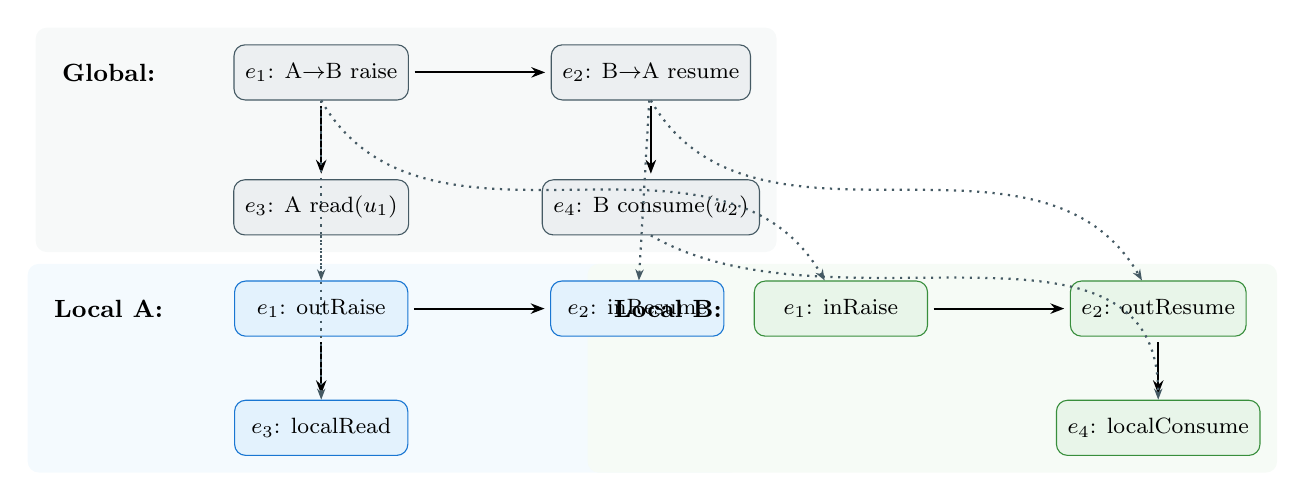
\begin{tikzpicture}[
  node distance=1.0cm and 1.8cm,
  pevt/.style={evtnode, minimum width=2.2cm},
  >=Stealth
]
\def\xLabel{-1.5}   % x-position for section labels
\def\xFirst{1.2}    % x-position for first event column
\def\yGlobal{2.5}   % y-position for Global row
\def\yLocalA{-0.5}  % y-position for Local A row
\def\xLocalBFirst{7.8} % x-position for Local B first event

%% Global Nodes
\node[font=\small\bfseries] (glabel) at (\xLabel, \yGlobal) {Global:};
\node[pevt, fill=palGrayLt, draw=palGray] (g1) at (\xFirst, \yGlobal) {$e_1$: A$\to$B raise};
\node[pevt, fill=palGrayLt, draw=palGray, right=of g1] (g2) {$e_2$: B$\to$A resume};
\node[pevt, fill=palGrayLt, draw=palGray, below=of g1] (g3) {$e_3$: A read($u_1$)};
\node[pevt, fill=palGrayLt, draw=palGray, below=of g2] (g4) {$e_4$: B consume($u_2$)};
\draw[stdarrow] (g1) -- (g2);
\draw[stdarrow] (g1) -- (g3);
\draw[stdarrow] (g2) -- (g4);

%% Local A Nodes
\node[font=\small\bfseries] (alabel) at (\xLabel, \yLocalA) {Local A:};
\node[pevt, fill=palBlueLt, draw=palBlue] (a1) at (\xFirst, \yLocalA) {$e_1$: outRaise};
\node[pevt, fill=palBlueLt, draw=palBlue, right=of a1] (a2) {$e_2$: inResume};
\node[pevt, fill=palBlueLt, draw=palBlue, below=0.8cm of a1] (a3) {$e_3$: localRead};
\draw[stdarrow] (a1) -- (a2);
\draw[stdarrow] (a1) -- (a3);

%% Local B Nodes
\node[pevt, fill=palGreenLt, draw=palGreen] (b1) at (\xLocalBFirst, \yLocalA) {$e_1$: inRaise};
\node[font=\small\bfseries, anchor=east] (blabel) at ([xshift=-8pt]b1.west) {Local B:};
\node[pevt, fill=palGreenLt, draw=palGreen, right=of b1] (b2) {$e_2$: outResume};
\node[pevt, fill=palGreenLt, draw=palGreen, below=0.8cm of b2] (b4) {$e_4$: localConsume};
\draw[stdarrow] (b1) -- (b2);
\draw[stdarrow] (b2) -- (b4);

%% Backgrounds
\begin{scope}[on background layer]
  \node[rounded corners, fill=palGrayLt!40, fit=(glabel)(g1)(g2)(g3)(g4), inner sep=6pt] {};
  \node[rounded corners, fill=palBlueLt!40, fit=(alabel)(a1)(a2)(a3), inner sep=6pt] {};
  \node[rounded corners, fill=palGreenLt!40, fit=(blabel)(b1)(b2)(b4), inner sep=6pt] {};
\end{scope}

%% Projection Arrows
\draw[stutterarrow, palGray] (g1) -- (a1);
\draw[stutterarrow, palGray] (g2) -- (a2);
\draw[stutterarrow, palGray] (g3) -- (a3);
\draw[stutterarrow, palGray] (g1.south) to[out=-60, in=120] (b1);
\draw[stutterarrow, palGray] (g2.south) to[out=-60, in=120] (b2);
\draw[stutterarrow, palGray] (g4.south) to[out=-30, in=90] (b4);
\end{tikzpicture}
\caption{Projection: a global script decomposes into local scripts for each role.}
\label{fig:projection}
\end{figure}

\begin{theorem}[Projection Preserves Well-Formedness]\label{thm:proj-wf}
If $\mathit{WF}(S)$ then $\mathit{WF}(\mathit{Proj}(S, r))$ for all roles $r$. \emph{(Mechanized: \texttt{project\_wellFormed}, Script.lean.)}
\end{theorem}

\begin{theorem}[Projection Preserves Traces]\label{thm:proj-traces}
If $\mathit{tr}$ is a valid trace of $S$, then $\mathit{traceProj}(S, r, \mathit{tr})$ is a valid trace of $\mathit{Proj}(S, r)$. \emph{(Mechanized: \texttt{proj\_validTrace}, Script.lean.)}
\end{theorem}

\begin{corollary}[Global Conformance Implies Local]\label{cor:global-implies-local}
If $S$ globally conforms on trace $\mathit{tr}$, then $S$ locally conforms for every role $r$ on $\mathit{traceProj}(S, r, \mathit{tr})$. \emph{(Mechanized: \texttt{proj\_localConform\_of\_globalConform}, Script.lean.)}
\end{corollary}

\begin{definition}[Trace Projection]\label{def:trace-projection}
$\mathit{traceProj}(S, r, \mathit{tr}) = \mathit{tr}.\texttt{filter}(\mathit{relevant}(r, \cdot))$.
\end{definition}

\begin{definition}[Local Conformance]\label{def:local-conformance}
Script $S$ \emph{locally conforms} for role $r$ on trace $\mathit{tr}$, written $\mathit{localConform}(S, r, \mathit{tr})$, if $\mathit{Proj}(S, r)$ is well-formed and $\mathit{tr}$ is a valid trace of $\mathit{Proj}(S, r)$.
\end{definition}

\subsection{PTB Compilation}\label{sec:ptb-compilation}

A coordination script's event structure admits many valid linearizations---any topological sort of the causal DAG respects the partial order. On-chain validators, however, need a single concrete command sequence to replay and verify. PTB compilation selects one such linearization and encodes it as a Programmable Transaction Block (PTB), inspired by Sui's transaction format~\cite{Blackshear2023}: a sequence of commands where each command produces a result stored in a numbered register $\mathit{Result}(i)$, and later commands reference earlier results as inputs, creating an explicit dataflow graph.

The key property is determinism. The event structure captures what \emph{could} happen; the PTB captures what \emph{did} happen. This determinism is what makes on-chain validation possible: validators replay the exact command sequence and verify that the result matches the proof. The correctness criterion is that the PTB's induced event structure (derived from its dependency and conflict relations) is well-formed and admits the PTB's command sequence as a valid trace (Theorems~\ref{thm:toscript-wf}--\ref{thm:valid-trace-trace}). A concrete worked example appears in \cref{sec:worked-example}; the formal definitions follow. All definitions and theorems are mechanized in \texttt{PTB.lean}.

\subsubsection{Command Model}\label{sec:command-model}

\begin{definition}[Command]\label{def:command}
A command is a triple $c = (\mathit{action}, \mathit{uses}, \mathit{conflicts})$ where $\mathit{action} : \mathit{Action}$, $\mathit{uses} : \Pfin(\NN)$ identifies result registers consumed as inputs, and $\mathit{conflicts} : \Pfin(\NN)$ records explicit conflict edges.
\end{definition}

\begin{definition}[Program]\label{def:program}
A PTB program is a list of commands $P = [c_0, \ldots, c_{n-1}]$. Command $c_i$ stores its output in register $\mathit{Result}(i)$, and may reference $\mathit{Result}(j)$ for $j \in c_i.\mathit{uses}$. Well-formedness requires $j < i$ for every $j \in c_i.\mathit{uses}$.
\end{definition}

\begin{definition}[Config]\label{def:config}
A PTB configuration $(\mathit{roles}, \mathit{roleKind})$ maps identifiers to roles and roles to kinds, connecting the PTB to the coordination layer's role structure. (In the Lean mechanization, this corresponds to \texttt{structure Config} in PTB.lean; an extended variant \texttt{AccessConfig} adds $\mathit{utxoRole}$ and $\mathit{ifaceRole}$ mappings used by the witness construction theorems.)
\end{definition}

\subsubsection{Derived Relations}\label{sec:derived-relations}

Given a program $P$, we derive three dependency relations ($\mathit{dataDep}$, $\mathit{utxoDep}$, $\mathit{handlerDep}$) that contribute to the causal order, plus one conflict marker ($\mathit{explicitConflict}$) for choice branches, and combine these into two structural relations: $\mathit{orderRel}$ (causal order) and $\mathit{conflictRel}$ (mutual exclusion). Each action~$a$ exposes accessor functions: $a.\mathit{readUtxos}$, $a.\mathit{writeUtxos}$, $a.\mathit{consumedUtxos}$, $a.\mathit{ifaceUses}$, $a.\mathit{ifaceInstalls}$, $a.\mathit{ifaceUninstalls}$.

\begin{definition}[Dependencies]\label{def:dependencies}
For commands $c_i, c_j$ with $i < j$:
\begin{itemize}
  \item $\mathit{dataDep}(i, j) \iff i \in c_j.\mathit{uses}$ --- result register dependency.
  \item $\mathit{utxoDep}(i, j) \iff c_i.\mathit{writeUtxos} \cap c_j.\mathit{utxoAccesses} \neq \emptyset \;\lor\; c_j.\mathit{writeUtxos} \cap c_i.\mathit{utxoAccesses} \neq \emptyset$ --- read-write or write-write overlap.
  \item $\mathit{handlerDep}(i, j) \iff c_i.\mathit{ifaceInstalls} \cap c_j.\mathit{ifaceUses} \neq \emptyset \;\lor\; c_i.\mathit{ifaceUses} \cap c_j.\mathit{ifaceUninstalls} \neq \emptyset$ --- install-before-use or use-before-uninstall.
\end{itemize}
\end{definition}

\begin{definition}[Order Relation]\label{def:order-rel}
$\mathit{orderRel}(i, j) \iff i < |P| \wedge j < |P| \wedge i < j \wedge (\mathit{dataDep}(i,j) \lor \mathit{utxoDep}(i,j) \lor \mathit{handlerDep}(i,j))$.
\end{definition}

\begin{definition}[Conflict Relation]\label{def:conflict-rel}
$\mathit{conflictRel}(i, j) \iff i < |P| \wedge j < |P| \wedge i \neq j \wedge (c_i.\mathit{consumedUtxos} \cap c_j.\mathit{consumedUtxos} \neq \emptyset \lor c_i.\mathit{ifaceInstalls} \cap c_j.\mathit{ifaceInstalls} \neq \emptyset \lor \mathit{explicitConflict}(i, j))$.
\end{definition}

\begin{remark}[Hereditary Conflict]\label{rem:conflict-properties}
The relation $\mathit{conflictRel}$ is symmetric (by commutativity of set intersection and the $i \neq j$ guard) and irreflexive (since $i \neq j$ is required), but does \emph{not} enforce hereditary conflict (downward closure of conflict under causality), as required by Winskel's original event structures~\cite{Winskel1986}. In Winskel's formulation, if $e \mathrel{\#} e'$ and $e' \leq e''$, then $e \mathrel{\#} e''$: conflict propagates forward through causality. ICE-UTxO omits this because: (i)~PTB-derived event structures have finite, acyclic order relations where the precedence graph's acyclicity check (\cref{def:ledger-invariant}, component~6) is sufficient for serializability without hereditary closure; (ii)~the serializability proof (\cref{thm:strong-serial}) depends on $\mathit{fullConflicts}$ symmetry and $\mathit{CoreState}$ commutativity, not on hereditary propagation; and (iii)~the projection theorems (\cref{thm:proj-wf,thm:proj-traces}) hold for the weaker conflict relation. Adding hereditary closure would strengthen the specification against modeling errors in hand-written scripts (where causal chains might introduce implicit conflicts) and is planned (\cref{sec:discussion}). For PTB-compiled scripts, the omission has no effect on the mechanized results: the $\mathit{toScript}$ translation produces conflict edges only between commands at the same causal depth, so hereditary closure would add no new edges.
\end{remark}

\subsubsection{Translation to Event Structure}\label{sec:translation}

\begin{definition}[toScript]\label{def:toscript}
Given configuration $\mathit{cfg}$ and program $P$, the induced script is:
\[
\mathit{toScript}(\mathit{cfg}, P) = (\mathit{cfg}.\mathit{roles}, \mathit{cfg}.\mathit{roleKind}, \{0, \ldots, |P|-1\}, \lambda i.\, c_i.\mathit{action}, \mathit{orderRel}, \mathit{conflictRel})
\]
\end{definition}

\begin{remark}[Compilation Direction]\label{rem:compilation-direction}
The translation is deliberately from programs to event structures, not the reverse. The PTB program is the author-facing artifact: it specifies \emph{what to execute} (commands with explicit data and conflict dependencies). The event structure extracted by $\mathit{toScript}$ is the verification artifact: it specifies \emph{what constraints the execution must satisfy} (causal order and conflict). The correctness theorem (\cref{thm:toscript-wf}) ensures that the extracted constraints are well-formed. A reverse direction---compiling an arbitrary event structure into a PTB---would require solving a scheduling problem (topological sort with conflict handling and register assignment) and is not needed for the protocol: transaction authors construct PTB programs directly or via a high-level DSL (\cref{sec:discussion}), and the ledger verifies the induced event structure. The design parallels the relationship between programs and their verification conditions in Hoare logic: the program is primary, the specification is derived.
\end{remark}

\begin{theorem}[toScript Well-Formedness]\label{thm:toscript-wf}
If $P$ satisfies $\mathit{rolesOK}$ and $\mathit{roleKindOK}$ with respect to $\mathit{cfg}$, then $\mathit{toScript}(\mathit{cfg}, P)$ is well-formed. \emph{(Mechanized: \texttt{Program.toScript\_wellFormed}, PTB.lean.)}
\end{theorem}

\begin{proof}[Proof sketch]
The seven well-formedness predicates decompose as follows. \textbf{WF-Order} and \textbf{WF-Conflict}: both endpoints are in $\{0, \ldots, |P|-1\}$ by the bound guards in the relation definitions. \textbf{WF-Irrefl} and \textbf{WF-Symm} for conflict: irreflexivity follows from $i \neq j$; symmetry from \texttt{conflictRel\_symm}. \textbf{WF-Acyclic}: if $\mathit{orderRel}^+(i, i)$ held, then $i < i$ by transitivity of the $i < j$ constraint in each order edge---contradiction. \textbf{WF-Roles} and \textbf{WF-RoleKind}: by hypothesis.
\end{proof}

\subsubsection{Valid Traces and Witness Construction}\label{sec:valid-traces}

\begin{figure}[t]
\centering
\begin{adjustbox}{max width=\linewidth, center}
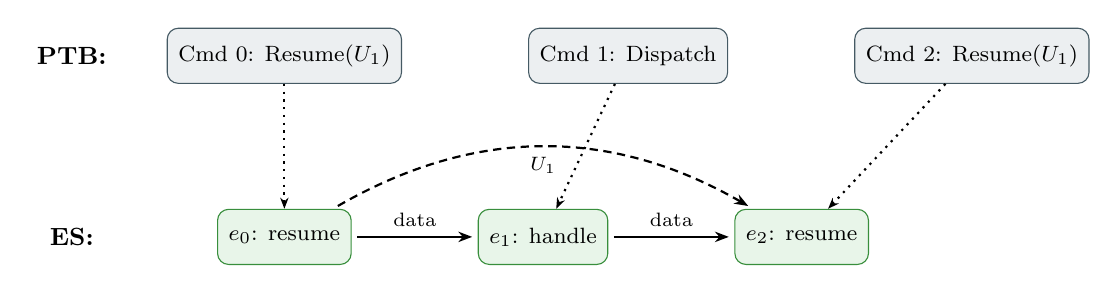
\begin{tikzpicture}[
  node distance=0.8cm and 1.6cm,
  >=Stealth
]
\def\xLabel{-1.2}  % x-position for row labels
\def\xFirst{1.5}   % x-position for first command/event
\def\yPTB{1.8}     % y-position for PTB row
\def\yES{-0.5}     % y-position for ES row

%% PTB Row
\node[font=\small\bfseries] at (\xLabel, \yPTB) {PTB:};
\node[evtnode, fill=palGrayLt, draw=palGray] (c0) at (\xFirst, \yPTB) {Cmd 0: Resume($U_1$)};
\node[evtnode, fill=palGrayLt, draw=palGray, right=of c0] (c1) {Cmd 1: Dispatch};
\node[evtnode, fill=palGrayLt, draw=palGray, right=of c1] (c2) {Cmd 2: Resume($U_1$)};

%% ES Row
\node[font=\small\bfseries] at (\xLabel, \yES) {ES:};
\node[evtnode, fill=palGreenLt, draw=palGreen] (e0) at (\xFirst, \yES) {$e_0$: resume};
\node[evtnode, fill=palGreenLt, draw=palGreen, right=of e0] (e1) {$e_1$: handle};
\node[evtnode, fill=palGreenLt, draw=palGreen, right=of e1] (e2) {$e_2$: resume};

%% Data Edges
\draw[stdarrow] (e0) -- node[above, font=\scriptsize] {data} (e1);
\draw[stdarrow] (e1) -- node[above, font=\scriptsize] {data} (e2);
\draw[stdarrow, densely dashed, bend left=30] (e0) to node[below, font=\scriptsize] {$U_1$} (e2);

%% Mapping Arrows
\draw[stutterarrow] (c0) -- (e0);
\draw[stutterarrow] (c1) -- (e1);
\draw[stutterarrow] (c2) -- (e2);
\end{tikzpicture}
\end{adjustbox}
\caption{PTB compilation mapping commands to event structures.}
\label{fig:ptb-compilation}
\end{figure}

\begin{theorem}[validTrace\_trace]\label{thm:valid-trace-trace}
If $P$ has no conflicts, then the full program-order trace $[0, \ldots, |P|-1]$ is a valid trace of $\mathit{toScript}(\mathit{cfg}, P)$. \emph{(Mechanized: \texttt{Program.validTrace\_trace}, PTB.lean.)}
\end{theorem}

\begin{theorem}[witnessGlobalOK\_of]\label{thm:witness-global-ok}
If $P$ satisfies $\mathit{rolesOK}$, $\mathit{roleKindOK}$, $\mathit{conflictFree}(\mathit{keep})$, and $\mathit{downClosed}(\mathit{keep})$, then $\mathit{toWitness}(\mathit{cfg}, P, \mathit{keep})$ is globally OK. \emph{(Mechanized: \texttt{Program.witnessGlobalOK\_of}, PTB.lean.)}
\end{theorem}

\begin{theorem}[validTrace\_traceOf]\label{thm:valid-trace-traceof}
Given a predicate $\mathit{keep} : \NN \to \mathit{Bool}$ such that $P$ is conflict-free on $\mathit{keep}$ and $\mathit{keep}$ is down-closed with respect to $\mathit{orderRel}$, the filtered trace $P.\mathit{traceOf}(\mathit{keep})$ is a valid trace of $\mathit{toScript}(\mathit{cfg}, P)$. \emph{(Mechanized: \texttt{Program.validTrace\_traceOf}, PTB.lean.)}
\end{theorem}

\begin{theorem}[crossRoleSafe\_of\_access]\label{thm:cross-role-safe}
If every command's access roles are contained in its participant set ($\mathit{accessRolesOK}$) and explicit conflicts are shared ($\mathit{explicitConflictShared}$), then conflicting commands always share at least one role. \emph{(Mechanized: \texttt{Program.crossRoleSafe\_of\_access}, PTB.lean.)}
\end{theorem}

\paragraph{Choice and the \texttt{keep} predicate.} The predicate $\mathit{keep} : \NN \to \mathit{Bool}$ selects which commands in a PTB are executed in a given run, modeling branching and conditional logic. For a linear protocol (no choices), $\mathit{keep} = \lambda i.\, \mathit{true}$. For a protocol with an exclusive choice between commands $i$ and $j$ (expressed via $\mathit{conflictRel}(i, j)$), exactly one of $\mathit{keep}(i)$ or $\mathit{keep}(j)$ is true. The two well-formedness conditions---$\mathit{keep}$ is conflict-free (no two kept commands conflict) and down-closed (if command $j$ is kept and $i \mathrel{\mathit{orderRel}} j$, then $i$ is kept)---ensure that the selected subset forms a valid configuration of the induced event structure (\cref{def:configuration}). The transaction author constructs $\mathit{keep}$ during execution (it records which branches were taken) and includes it in the coordination witness. The IVC proof then certifies that the selected commands were executed correctly, binding $\mathit{keep}$ into the $\mathit{commitHash}$ so the ledger cannot be tricked into accepting an inconsistent subset.

\subsubsection{Worked Example}\label{sec:worked-example}

Consider the collateralized loan scenario from \cref{sec:problem}, compiled to a 3-command PTB:

\begin{table}[h]
\centering\small
\begin{tabular}{cllcc}
\toprule
$i$ & \textbf{Command} & \textbf{Action} & \textbf{uses} & \textbf{conflicts} \\
\midrule
0 & Resume borrower coroutine & $\texttt{resume}(r_b, r_o, \mathit{oracle}, \mathit{getPrice})$ & $\emptyset$ & $\emptyset$ \\
1 & Dispatch to price handler & $\texttt{raise}(r_o, r_h, \mathit{oracle}, \mathit{dispatch})$ & $\{0\}$ & $\emptyset$ \\
2 & Resume with price result & $\texttt{resume}(r_h, r_b, \mathit{oracle}, \mathit{result})$ & $\{1\}$ & $\emptyset$ \\
\bottomrule
\end{tabular}
\end{table}

\paragraph{Derived edges.} $\mathit{dataDep}(0,1)$ since $0 \in c_1.\mathit{uses}$; $\mathit{dataDep}(1,2)$ since $1 \in c_2.\mathit{uses}$; $\mathit{handlerDep}(0,2)$ since both access the oracle interface. Thus $\mathit{orderRel} = \{(0,1), (1,2), (0,2)\}$ and $\mathit{conflictRel} = \emptyset$.

\paragraph{Induced script.} $\mathit{toScript}$ produces events $\{0,1,2\}$ with order $0 < 1 < 2$ (plus $0 < 2$) and no conflict. This is a total order, so the unique valid trace is $[0,1,2]$.

\paragraph{Validity.} Since $\mathit{conflictRel} = \emptyset$, \cref{thm:valid-trace-trace} applies directly: the program-order trace $[0,1,2]$ is valid. By \cref{thm:witness-global-ok}, $\mathit{toWitness}(\mathit{cfg}, P, \lambda i.\, \mathit{true})$ is globally OK.

\paragraph{Step-by-step configuration sequence.} We can trace the execution through the formal definitions. Starting from the empty configuration $C_0 = \emptyset$: event~$0$ (resume borrower) is enabled in $C_0$ because it has no predecessors and no conflicts, so $C_1 = \{0\}$. Event~$1$ (dispatch to handler) is enabled in $C_1$ because its sole predecessor~$0$ is present, so $C_2 = \{0, 1\}$. Event~$2$ (resume with result) is enabled in $C_2$ because predecessors~$0$ and~$1$ are both present, so $C_3 = \{0, 1, 2\}$. The configuration $C_3$ is maximal (all events have occurred), confirming that the trace $[0, 1, 2]$ is complete.

\paragraph{Connection to the witness.} The valid trace $[0, 1, 2]$ is exactly the evidence packaged into the coordination witness $W = (S, [0, 1, 2])$, which the IVC proof then certifies. A verifier need not re-execute the three commands; it checks that $W$ satisfies $\mathit{witnessGlobalOK}$ (which reduces to checking that $[0,1,2]$ is a valid trace of the induced script $S$) and that the IVC proof attests to the computation's correctness.

\paragraph{What the IVC proof certifies.} The transaction author generates an IVC proof certifying: (i)~the borrower's coroutine correctly computed the loan terms from the price data (execution correctness); (ii)~the price-oracle effect was dispatched to the correct handler and the result propagated (effect resolution); and (iii)~the witness $W = (S, [0,1,2])$ satisfies $\mathit{witnessGlobalOK}$ (protocol conformance). The $\mathit{commitHash}$ binds this proof to the specific input UTxOs (borrower's collateral, oracle's price feed) and output UTxOs (the loan position, updated collateral). A validator checks the IVC proof and the structural predicates ($\mathit{commitEnabledStrong}$) without re-executing the coroutine logic.

\paragraph{Shard-local verification.} Suppose the borrower resides on shard~1 and the oracle on shard~2. Under S-BAC (\cref{sec:sbac-integration}), shard~1 checks: (i)~$\mathit{witnessLocalOK}$ for the borrower role $r_b$---that the projected trace $[0, 2]$ locally conforms to $\mathit{Proj}(S, r_b)$; and (ii)~that the borrower's input UTxOs are live. Shard~2 checks the same for oracle role $r_o$ with projected trace $[0, 1]$. By \cref{thm:global-implies-local}, these local checks are implied by the global witness validity; by \cref{thm:consistent-implies-global}, their conjunction (plus trace consistency) recovers the global guarantee. Neither shard needs to see the other's UTxO set or re-execute the other's coroutine steps.

\subsection{S-BAC Integration}\label{sec:sbac-integration}

When a transaction's participants span multiple shards---for example, a borrower on shard~1 and an oracle on shard~2---the transaction cannot be validated by a single shard. The shards must synchronize to ensure atomicity: either all shards commit, or all abort. This is the classic atomic commit problem, complicated by the possibility of Byzantine (adversarial) faults.

Sharded Byzantine Atomic Commit (S-BAC), introduced by Chainspace~\cite{AlBassam2018}, addresses this with a two-phase protocol. In the \emph{prepare} phase, each shard independently checks its local portion of the transaction (local trace conformance for its roles and UTxO liveness for its inputs). In the \emph{accept} phase, if all shards prepared successfully, the transaction commits; if any shard aborts, all abort. This is similar to classical two-phase commit (2PC) but tolerant of Byzantine faults within each shard's BFT consensus.

ICE-UTxO improves over Chainspace's original design in one key respect: in Chainspace, each shard re-executes the transaction's logic during prepare. In ICE-UTxO, shards only check their local trace conformance (is my role following the protocol?) and UTxO liveness (are the inputs still unspent?). The heavy computation---verifying that the full interleaving respects the coordination script---is certified by the IVC proof, which shards verify rather than re-execute. This reduces both the computation overhead per shard and the amount of private data that must be revealed.

The definitions below formalize how coordination witnesses connect to the S-BAC commit decision.

\begin{definition}[S-BAC Configuration]\label{def:sbac-config}
An S-BAC configuration is a pair $(\mathit{shardOfUtxo}, \mathit{rolesOfShard})$ mapping UTxOs to shards and shards to their associated roles.
\end{definition}

\begin{definition}[Coordination Witness]\label{def:coord-witness}
A coordination witness is a pair $W = (S, \mathit{tr})$ of a script $S$ and a trace $\mathit{tr}$.
\end{definition}

\begin{definition}[Witness Predicates]\label{def:witness-predicates}
\begin{align*}
\mathit{witnessGlobalOK}(W) &\iff S.\mathit{globalConform}(\mathit{tr}) \\
\mathit{witnessLocalOK}(W) &\iff \forall r \in S.\mathit{roles}.\; S.\mathit{localConform}(r, S.\mathit{traceProj}(r, \mathit{tr})) \\
\mathit{witnessConsistent}(W) &\iff S.\mathit{traceConsistent}(\mathit{tr})
\end{align*}
\end{definition}

\begin{theorem}[Global Implies Local]\label{thm:global-implies-local}
$\mathit{witnessGlobalOK}(W) \implies \mathit{witnessLocalOK}(W)$. \emph{(Mechanized: \texttt{witnessLocalOK\_of\_global}, SBAC.lean.)}
\end{theorem}

\begin{theorem}[Consistent Implies Global]\label{thm:consistent-implies-global}
If $S$ is well-formed and $\mathit{witnessConsistent}(W)$, then $\mathit{witnessGlobalOK}(W)$. \emph{(Mechanized: \texttt{witnessGlobalOK\_of\_local\_and\_consistent}, SBAC.lean.)}
\end{theorem}

\begin{definition}[Coordination Transaction]\label{def:coord-tx}
A coordination transaction pairs a ledger transaction with a witness: $\mathit{ctx} = (\mathit{tx}, W)$.
\end{definition}

\begin{definition}[Coordinated Commit]\label{def:coord-commit}
Commit is enabled if the ledger commit guard passes \emph{and} the witness validates:
\[
\mathit{coordCommitEnabled}(m, L, \mathit{ctx}) \iff \mathit{commitEnabledStrong}(m, L, \mathit{tx}) \wedge \mathit{witnessGlobalOK}(W)
\]
\end{definition}

\begin{definition}[Shard-Local Check]\label{def:shard-local-check}
During S-BAC prepare, shard $s$ checks:
\begin{enumerate}
  \item \textbf{Local trace conformance}: for every role $r$ associated with $s$, $\mathit{localConform}(S, r, \mathit{traceProj}(S, r, \mathit{tr}))$.
  \item \textbf{UTxO liveness}: inputs assigned to shard $s$ are in $L.\mathit{utxos}$.
\end{enumerate}
\end{definition}

\begin{theorem}[Local Sufficiency]\label{thm:local-sufficiency}
If $\mathit{coordCommitEnabled}(m, L, \mathit{ctx})$ holds, then $\mathit{coordCommitEnabledLocal}(m, L, \mathit{ctx})$ holds; that is, shard-local checks are sufficient when the global witness is valid. \emph{(Mechanized: \texttt{coordCommitEnabledLocal\_of\_global}, SBAC.lean.)}
\end{theorem}

The definitions and theorems in this section establish \emph{safety} properties: the model specifies what constitutes a valid execution and proves that the commit mechanism admits only valid executions. Conditional \emph{liveness} properties---guaranteeing that well-formed protocols eventually complete under fairness assumptions---are established in \cref{sec:liveness} using TLA-style reasoning with mechanized support lemmas and TLC model-checking validation.

\begin{figure}[t]
\centering
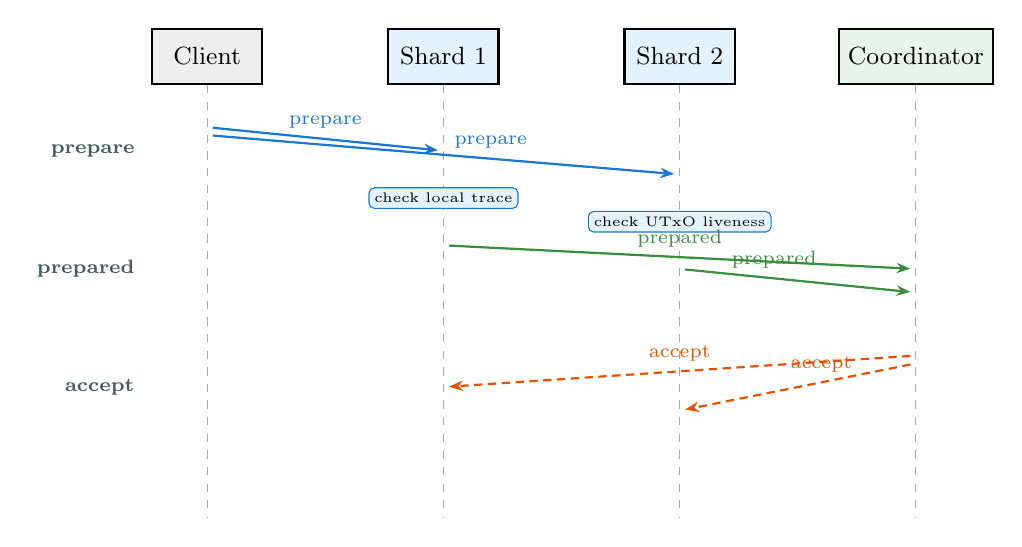
\begin{tikzpicture}[>=Stealth]
% Actor x-positions
\def\xClient{0}    \def\xSOne{3}
\def\xSTwo{6}      \def\xCoord{9}
% Phase y-positions
\def\yPrepare{-1.2}   \def\yPrepared{-2.7}   \def\yAccept{-4.2}

%% Actors
\node[actornode, fill=palGrayLt]  (client) at (\xClient, 0) {Client};
\node[actornode, fill=palBlueLt]  (s1)     at (\xSOne, 0)   {Shard 1};
\node[actornode, fill=palBlueLt]  (s2)     at (\xSTwo, 0)   {Shard 2};
\node[actornode, fill=palGreenLt] (coord)  at (\xCoord, 0)  {Coordinator};

%% Lifelines
\foreach \n in {client, s1, s2, coord} {
  \draw[dashed, palGray!50] (\n.south) -- ++(0, -5.5);
}

%% Phase Labels
\node[font=\scriptsize\bfseries, palGray, anchor=east] at (-0.8, \yPrepare)  {prepare};
\node[font=\scriptsize\bfseries, palGray, anchor=east] at (-0.8, \yPrepared) {prepared};
\node[font=\scriptsize\bfseries, palGray, anchor=east] at (-0.8, \yAccept)   {accept};

%% Messages — Phase 1: prepare
\draw[stdarrow, palBlue] (\xClient, -0.9) -- node[above, font=\scriptsize] {prepare} (\xSOne, \yPrepare);
\draw[stdarrow, palBlue] (\xClient, -1.0) -- node[above, font=\scriptsize, pos=0.6] {prepare} (\xSTwo, -1.5);

% Shard annotations
\node[rounded corners=2pt, fill=palBlueLt, draw=palBlue, font=\tiny, inner sep=2pt]
  at (\xSOne, -1.8) {check local trace};
\node[rounded corners=2pt, fill=palBlueLt, draw=palBlue, font=\tiny, inner sep=2pt]
  at (\xSTwo, -2.1) {check UTxO liveness};

%% Messages — Phase 2: prepared
\draw[stdarrow, palGreen] (\xSOne, -2.4) -- node[above, font=\scriptsize] {prepared} (\xCoord, \yPrepared);
\draw[stdarrow, palGreen] (\xSTwo, \yPrepared) -- node[above, font=\scriptsize, pos=0.4] {prepared} (\xCoord, -3.0);

%% Messages — Phase 3: accept
\draw[stdarrow, densely dashed, palOrange] (\xCoord, -3.8) -- node[above, font=\scriptsize] {accept} (\xSOne, \yAccept);
\draw[stdarrow, densely dashed, palOrange] (\xCoord, -3.9) -- node[above, font=\scriptsize, pos=0.4] {accept} (\xSTwo, -4.5);
\end{tikzpicture}
\caption{S-BAC prepare flow for ICE-UTxO. Dashed vertical lines are lifelines; three temporal phases flow top-to-bottom.}
\label{fig:sbac}
\end{figure}

%% ═══════════════════════════════════════════════════════════════════════════
\section{Operational Semantics and Ledger Safety}\label{sec:opsem}

The preceding sections defined \emph{what} ICE-UTxO transactions look like---state components, coordination scripts, event structures, and compiled PTB programs. This section defines \emph{how} those transactions change the ledger: a small-step operational semantics with eight constructors, two concurrency modes, and six invariants preserved by every step. All definitions and theorems are mechanized in \texttt{StarstreamPilot.lean}.

\subsection{Transaction Lifecycle}\label{sec:lifecycle}

\emph{Running example.} Consider the collateralized loan liquidation from \cref{sec:problem} and its PTB program from \cref{sec:worked-example}. The transaction would progress through the lifecycle below as follows: submit to pending (\texttt{addPending}), acquire locks on the oracle and borrower UTxOs (\texttt{lockInputs}), install the price handler (\texttt{installH}), raise the price query (\texttt{raiseE}), dispatch the handler (\texttt{handleE}), and finally commit with the IVC proof (\texttt{commit}).

A transaction proceeds through seven phases: Idle, Reserve, Executing, Committing, Committed, Rollback, and Failed.

\begin{figure}[t]
\centering
\begin{adjustbox}{max width=\linewidth, center}
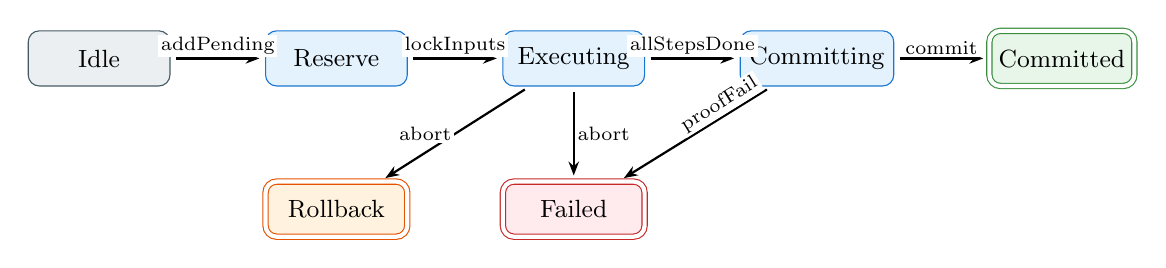
\begin{tikzpicture}[
  fsmst/.style={fsmstate, minimum width=1.8cm},
  >=Stealth,
  node distance=1.2cm
]
%% Happy Path Nodes
\node[fsmst, fill=palGrayLt, draw=palGray] (idle) {Idle};
\node[fsmst, fill=palBlueLt, draw=palBlue, right=of idle] (reserve) {Reserve};
\node[fsmst, fill=palBlueLt, draw=palBlue, right=of reserve] (exec) {Executing};
\node[fsmst, fill=palBlueLt, draw=palBlue, right=of exec] (commit) {Committing};
\node[fsmst, fill=palGreenLt, draw=palGreen, double, double distance=1.5pt, right=of commit] (done) {Committed};
%% Failure Nodes
\node[fsmst, fill=palOrangeLt, draw=palOrange, double, double distance=1.5pt, below=of reserve] (roll) {Rollback};
\node[fsmst, fill=palRedLt, draw=palRed, double, double distance=1.5pt, below=of exec] (fail) {Failed};
%% Transitions
\draw[stdarrow] (idle) -- node[above, font=\scriptsize, fill=white, inner sep=1pt] {addPending} (reserve);
\draw[stdarrow] (reserve) -- node[above, font=\scriptsize, fill=white, inner sep=1pt] {lockInputs} (exec);
\draw[stdarrow] (exec) -- node[above, font=\scriptsize, fill=white, inner sep=1pt] {allStepsDone} (commit);
\draw[stdarrow] (commit) -- node[above, font=\scriptsize, fill=white, inner sep=1pt] {commit} (done);
\draw[stdarrow] (exec) -- node[left, font=\scriptsize, fill=white, inner sep=1pt] {abort} (roll);
\draw[stdarrow] (exec) -- node[right, font=\scriptsize, fill=white, inner sep=1pt] {abort} (fail);
\draw[stdarrow] (commit) -- node[above, font=\scriptsize, fill=white, inner sep=1pt, sloped, pos=0.3] {proofFail} (fail);
\end{tikzpicture}
\end{adjustbox}
\caption{Transaction lifecycle state machine.}
\label{fig:lifecycle}
\end{figure}

\begin{definition}[Step]\label{def:step}
The small-step relation $\mathit{Step} : \mathit{Mode} \to \mathit{Ledger} \to \mathit{Ledger} \to \text{Prop}$ has eight constructors in three groups: \emph{lifecycle} (addPending, lockInputs, commit, abort) governs transaction admission, resource reservation, finalization, and failure; \emph{effect} (installH, uninstallH, raiseE, handleE) implements the algebraic-effects paradigm at the ledger level; and the lifecycle constructors carry the mode-sensitive preconditions that enforce concurrency control.
\end{definition}

\begin{table}[t]
\caption{Step constructors of the ICE-UTxO operational semantics.}
\label{tab:step-constructors}
\centering\small
\begin{tabular}{lllll}
\toprule
\textbf{Constructor} & \textbf{Mode} & \textbf{Precondition} & \textbf{Effect} & \textbf{Intuition} \\
\midrule
\texttt{addPending} & any & $\mathit{tx} \notin L.\mathit{pending}$, \texttt{noDupProofs} & Add to pending & Submit for consideration \\
\texttt{lockInputs} & locking & $\mathit{tx} \in \mathit{pending}$, inputs disjoint, live & Lock inputs & Reserve inputs (pessimistic) \\
\texttt{commit} & any & \texttt{commitEnabledStrong}, acyclicity & Apply commit & Finalize---strongest gate \\
\texttt{abort} & any & $\mathit{tx} \in \mathit{pending}$ & Release locks & Graceful failure / timeout \\
\texttt{installH} & any & (none) & Push handler & Register effect handler \\
\texttt{uninstallH} & any & (none) & Pop handler & Deregister effect handler \\
\texttt{raiseE} & any & (none) & Push effect & Request cross-boundary service \\
\texttt{handleE} & any & effect + handler present & Route effect & Dispatch to registered handler \\
\bottomrule
\end{tabular}
\end{table}

\paragraph{Entry gate: \texttt{addPending}.} The \texttt{addPending} constructor admits transactions to the pending set. Its precondition---$\mathit{tx} \notin L.\mathit{pending}$ and \texttt{noDupProofs}---is deliberately minimal: any structurally well-formed transaction passes. No input liveness, proof validity, or phase correctness is checked here. All semantic validation is deferred to later lifecycle phases, keeping admission lightweight.

\begin{remark}[Security: Spam and DoS Surface]\label{rem:spam}
The \texttt{addPending} constructor admits any structurally well-formed transaction without checking proof validity or input liveness. This makes it the primary denial-of-service attack surface: an adversary can flood the pending set with transactions that will never commit. Mitigation via fees, rate limiting, or proof-of-work puzzles is essential in deployment but outside the model's scope.
\end{remark}

\paragraph{Pessimistic reserve: \texttt{lockInputs}.} The \texttt{lockInputs} constructor implements pessimistic concurrency control, reserving a transaction's inputs before execution begins. The preconditions---inputs disjoint from already-locked UTxOs and inputs live---mirror the lock-acquisition phase of strict two-phase locking (S2PL) in database systems. In the loan example, the borrower's collateral UTxO and the oracle's price-feed UTxO are locked before the price query is dispatched, ensuring that no concurrent transaction can consume them while the multi-step interaction is in progress.

\paragraph{Terminal gate: \texttt{commit}.} This is the hardest gate to pass. The \texttt{commit} constructor carries the strongest preconditions of any constructor. It requires: (i)~all proof commitments verified ($\mathit{allProofsVerified}$), (ii)~structural validity ($\mathit{validTx}$), (iii)~the transaction is in the committing phase, (iv)~the transaction is not already in the history, and (v)~both acyclicity predicates hold after appending. Each guard prevents a specific failure mode: (i)~blocks unverified computation, (ii)~blocks double-spends and stale inputs, (iii)~enforces lifecycle discipline, (iv)~prevents duplicate commits, and (v)~ensures the resulting history admits a conflict-serializable schedule (\cref{sec:serializability}).

\paragraph{Graceful failure: \texttt{abort}.} The \texttt{abort} constructor is intentionally nondeterministic: any pending transaction may abort at any time, modeling timeouts, cancellation, and resource limits. The safety philosophy is asymmetric: safety is not ``valid transactions must commit'' but ``only valid transactions \emph{can} commit.'' Making abort unconditional ensures that the model's safety proofs hold regardless of the abort policy a deployment chooses---whether time-based, fee-based, or operator-initiated.

\paragraph{Effect quartet: \texttt{installH}, \texttt{uninstallH}, \texttt{raiseE}, \texttt{handleE}.} These four constructors implement the algebraic-effects paradigm at the ledger level. In the loan example, the sequence is: (1)~\texttt{installH} registers a price-oracle handler on the oracle interface; (2)~\texttt{raiseE} raises a ``get price'' effect on that interface; (3)~\texttt{handleE} dispatches the effect to the installed handler, which produces the price data; (4)~optionally, \texttt{uninstallH} removes the handler after use. The constructors have no preconditions restricting their interleaving. In particular, an \texttt{uninstallH} step can remove a handler while a \texttt{raiseE} step targeting the same interface is pending. The model handles this by design: \texttt{handleE} requires both a pending effect and a handler to be present, so an uninstall-before-handle sequence simply leaves the effect unrouted, and the transaction must eventually abort or install a replacement handler.

\begin{remark}[Handler Stack Discipline]\label{rem:handler-stack}
The handler stack follows a LIFO (last-in, first-out) discipline: the most recently installed handler for an interface is the one that receives the next effect raised on that interface. This mirrors the handler-stack semantics of algebraic effect systems in programming languages (e.g., Eff, Koka, OCaml~5). The LIFO ordering interacts safely with concurrent uninstallation: if handler $h_1$ is installed, then $h_2$ is installed on the same interface, and $h_1$ is subsequently uninstalled, the stack pops $h_1$ but $h_2$ remains and continues to service effects. If \emph{all} handlers for an interface are uninstalled while effects are pending, the effects remain in the queue indefinitely; the transaction cannot reach the committing phase (since unrouted effects imply incomplete execution) and must eventually abort under $\mathit{WF}(\text{abort})$ (\cref{sec:liveness}).
\end{remark}

\begin{remark}[Effects and Commit Admissibility]\label{rem:effects-commit}
The commit guard $\mathit{commitEnabledStrong}$ (\cref{def:commit-enabled}) does not explicitly check for unresolved effects. Instead, effect resolution is enforced \emph{through the IVC proof}. The IVC proof predicate (\cref{rem:ivc-predicate}) includes effect resolution as a sub-goal: a valid proof certifies that every raised effect was dispatched and handled. A transaction with unresolved effects cannot produce a valid IVC proof, so $\mathit{allProofsVerified}$ will not hold, and the transaction cannot commit. This design keeps the commit guard lean (it checks a single cryptographic predicate rather than enumerating execution-level conditions) and places the burden of proving completeness on the transaction author's prover rather than on the on-chain validator. The connection is conditional on Security Assumption~1 (ZK verifier soundness): if the verifier is unsound, a transaction with unresolved effects could forge a proof and commit.
\end{remark}

\begin{definition}[State Updates]\label{def:state-updates}
\begin{align*}
\mathit{applyCommit}(L, \mathit{tx}) &= L\Big[\mathit{utxos} := (L.\mathit{utxos} \setminus \mathit{tx.inputs}) \cup \mathit{tx.outputs},\\
&\quad\; \mathit{consumed} := L.\mathit{consumed} \cup \mathit{tx.inputs},\\
&\quad\; \mathit{locked} := L.\mathit{locked} \setminus \mathit{tx.inputs},\\
&\quad\; \mathit{pending} := L.\mathit{pending} \setminus \{\mathit{tx}\},\\
&\quad\; \mathit{history} := L.\mathit{history} \mathbin{+\!\!+} [\mathit{tx}]\Big]
\end{align*}
\begin{align*}
\mathit{applyAbort}(L, \mathit{tx}) &= L\Big[\mathit{locked} := L.\mathit{locked} \setminus \mathit{tx.inputs},\;
\mathit{pending} := L.\mathit{pending} \setminus \{\mathit{tx}\}\Big]
\end{align*}
\end{definition}

\begin{definition}[Multi-Step]\label{def:multi-step}
$\mathit{Steps} : \mathit{Mode} \to \mathit{Ledger} \to \mathit{Ledger} \to \text{Prop}$ is the reflexive-transitive closure of $\mathit{Step}$.
\end{definition}

\subsection{Commit Rule and Proof-Gating}\label{sec:commit-rule}

The commit rule enforces that only proof-verified, structurally valid transactions can extend the ledger history.

\begin{definition}[All Proofs Verified]\label{def:all-proofs-verified}
$\mathit{allProofsVerified}(\mathit{tx}) \iff \mathit{tx.proofCommitments} \neq [] \wedge \forall p \in \mathit{tx.proofCommitments}.\; p.\mathit{phase} = \text{Verified}$
\end{definition}

\paragraph{Trust boundary.} The predicate $\mathit{allProofsVerified}$ checks phase flags set by an external ZK verifier. Cryptographic soundness---that a \texttt{Verified} flag genuinely corresponds to a valid ZK proof---is outside the scope of this formalization. The model proves: \emph{if} the verifier sets flags correctly, \emph{then} the ledger maintains its invariants.

\paragraph{IVC proof failure and timeout.} A proof commitment that fails during generation or verification transitions to the \texttt{Failed} phase (\cref{def:proof-commitment}). Since $\mathit{allProofsVerified}$ requires \emph{every} commitment to be in the \texttt{Verified} phase, any single proof failure prevents the transaction from committing. The transaction remains in the pending set until it is aborted. There is no partial-proof recovery: if $k$ of $n$ proofs verify but the remaining fail, the entire transaction must abort and retry.

\paragraph{Security assumptions.} The commit rule relies on assumptions SA1 (ZK verifier soundness), SA2 (phase discipline), and SA3 (S-BAC shard honesty) from \cref{sec:state-components}. These are not restated here; the single list in \cref{sec:state-components} is the authoritative reference.

\paragraph{Phase ordering in practice.} SA2 deserves elaboration. The \texttt{Step} relation is intentionally permissive: it does not constrain the order in which constructors are applied. For instance, nothing in the model prevents a \texttt{commit} step from being attempted before \texttt{lockInputs}---the preconditions will simply fail. This design keeps the formal model simple and makes the safety proofs independent of any particular scheduling strategy. However, a deployment must enforce the intended lifecycle (\cref{fig:lifecycle}) externally---for example, by wrapping the step constructors in a state-machine executor that rejects out-of-order transitions, or by encoding the lifecycle phases into the transaction type at the language level. The key guarantee is that even if a buggy executor applies steps in the wrong order, no invalid transaction can commit: the \texttt{commitEnabledStrong} guard (\cref{def:commit-enabled}) is the sole gateway. The safety proofs are therefore strictly stronger than a phase-restricted model would provide: they hold for the full state space, including all ill-phased interleavings, so any deployment that restricts to well-phased executions inherits the guarantees automatically as a corollary.

\paragraph{Security considerations.} Beyond SA1--SA3 (\cref{sec:state-components}), the operational semantics expose several attack surfaces that a deployment must address:
\begin{enumerate}
  \item \textbf{Griefing via lock exhaustion.} In locking mode, an adversary can submit transactions that lock high-demand UTxOs and then stall indefinitely (never committing or aborting). The model permits this because the \texttt{abort} constructor is nondeterministic---it does not fire automatically. A deployment must enforce lock timeouts (\cref{sec:ledger-invariants}) so that stalled locks are eventually released.
  \item \textbf{Front-running in optimistic mode.} An adversary who observes a pending transaction's read set can race to commit a conflicting transaction that invalidates the victim's snapshot, forcing an abort. Repeated front-running can starve a target transaction indefinitely. Mitigation strategies include commit-ordering fairness policies, encrypted mempools, or falling back to locking mode for high-value transactions.
  \item \textbf{Handler manipulation.} An adversary who can issue \texttt{installH} for an interface before a legitimate \texttt{raiseE} arrives can intercept the effect and route it to a malicious handler. The model places no restriction on who may install handlers; in a deployment, contract authors must restrict handler installation---e.g., to the roles designated in the coordination script (\cref{sec:coordination-witness}). The coordination script provides the formal mechanism for this restriction: the global type assigns roles to interfaces, and the projected local scripts specify which roles may install handlers on which interfaces. A shard checking $\mathit{witnessLocalOK}$ for its roles will reject a trace in which an unauthorized role installs a handler, because the projected trace will not conform to the local script. Handler authorization is thus enforced by the same witness-verification mechanism that enforces protocol compliance.
  \item \textbf{Proof forgery.} If the ZK verifier soundness assumption is violated (e.g., due to a bug in the proving circuit or a break in the underlying cryptographic primitive), an adversary can forge proof commitments and commit invalid transactions. All six ledger invariant components depend on proof-gating (\cref{thm:proof-gated}); a forged proof bypasses the only gate. Defense in depth---such as redundant verification by multiple independent provers---can mitigate this risk.
\end{enumerate}

\paragraph{On-chain verification.} A validator (or shard) processing a transaction checks three things: (i)~the IVC proof verifies under the stated $\mathit{verifyKey}$, attesting to execution correctness, effect resolution, and protocol conformance (\cref{rem:ivc-predicate}); (ii)~$\mathit{commitEnabledStrong}$ holds---inputs are live, outputs are fresh, the transaction is in the committing phase, and mode-specific conditions are satisfied (\cref{def:commit-enabled}); and (iii)~the coordination witness satisfies $\mathit{witnessGlobalOK}$, decomposed to shard-local checks via \cref{thm:global-implies-local}. Validators do \emph{not} re-execute coroutine logic, replay effect dispatch, or re-check the coordination protocol---all of this is covered by the IVC proof. The on-chain cost is dominated by proof verification (typically under 10ms for a Groth16 or Halo2 proof) plus the $\mathit{commitEnabledStrong}$ structural checks (set membership tests on UTxO identifiers).

\begin{definition}[Valid Transaction]\label{def:valid-tx}
$\mathit{validTx}(L, \mathit{tx})$ requires:
\begin{itemize}
  \item $\mathit{tx.inputs} \neq \emptyset$ and $\mathit{tx.outputs} \neq \emptyset$
  \item $\mathit{tx.inputs} \cap \mathit{tx.outputs} = \emptyset$ (inputs disjoint from outputs)
  \item $\mathit{tx.inputs} \subseteq L.\mathit{utxos}$ (inputs are live)
  \item $\mathit{tx.outputs} \cap (L.\mathit{utxos} \cup L.\mathit{consumed}) = \emptyset$ (outputs are fresh)
\end{itemize}
\end{definition}

\begin{remark}[Non-empty inputs]\label{rem:nonempty-inputs}
The requirement $\mathit{tx.inputs} \neq \emptyset$ excludes coinbase-style and minting transactions, which create outputs without consuming inputs. This is deliberate: ICE-UTxO models coordination among \emph{existing} UTxOs, and the serializability proof (\cref{sec:serializability}) relies on every committed transaction inducing at least one conflict edge in the precedence graph. Extending the model to handle coinbase transactions (which affect only outputs) is straightforward---they would be trivially serializable---but is outside the current scope. Cardano's minting policy scripts, which operate on a separate policy-id mechanism rather than the UTxO spend relation, are similarly excluded.
\end{remark}

\begin{definition}[Commit Enabled---Strong]\label{def:commit-enabled}
$\mathit{commitEnabledStrong}(m, L, \mathit{tx})$ holds if:
\[
\mathit{allProofsVerified}(\mathit{tx}) \wedge \mathit{validTx}(L, \mathit{tx}) \wedge \mathit{tx.phase} = \text{Committing} \wedge \mathit{tx} \notin L.\mathit{history}
\]
and additionally:
\begin{itemize}
  \item \textbf{Locking mode}: $\mathit{tx.inputs} \subseteq L.\mathit{locked}$ and $\mathit{tx.readSet} \subseteq L.\mathit{utxos}$.
  \item \textbf{Optimistic mode}: $\mathit{tx.readSet} \subseteq L.\mathit{utxos}$ and $\mathit{tx.outputs}$ are fresh.
\end{itemize}
\end{definition}

\begin{theorem}[Proof-Gated Commit]\label{thm:proof-gated}
Any step that extends the history requires proof verification:
\[
\mathit{Step}(m, L, L') \wedge L'.\mathit{history} = L.\mathit{history} \mathbin{+\!\!+} [\mathit{tx}] \implies \mathit{proofOk}(\mathit{tx})
\]
\emph{(Mechanized: \texttt{commit\_requires\_proof}, StarstreamPilot.lean.)}
\end{theorem}

\begin{proof}[Proof sketch]
Exhaustive case analysis on the eight \texttt{Step} constructors. Seven non-commit constructors leave the history unchanged, yielding a contradiction with the hypothesis via the lemma $\mathit{xs} \neq \mathit{xs} \mathbin{+\!\!+} [x]$. The commit constructor directly provides $\mathit{allProofsVerified}(\mathit{tx})$ from $\mathit{commitEnabledStrong}$.
\end{proof}

\subsection{Concurrency Modes}\label{sec:concurrency-modes}

ICE-UTxO supports two concurrency modes, selected per-transaction:

\paragraph{Locking mode} ($m = \text{locking}$). Inputs are reserved before execution via the \texttt{lockInputs} step, which requires $\mathit{tx.inputs} \cap L.\mathit{locked} = \emptyset$ (no double-locking) and $\mathit{tx.inputs} \subseteq L.\mathit{utxos}$ (inputs live). At commit time, the commit guard checks $\mathit{tx.inputs} \subseteq L.\mathit{locked}$.

\paragraph{Optimistic mode} ($m = \text{optimistic}$). No locks are acquired. At commit time, the guard checks that the read snapshot is still valid ($\mathit{tx.readSet} \subseteq L.\mathit{utxos}$) and outputs are still fresh. If the snapshot has been invalidated by a concurrent commit, the transaction fails.

Both modes are proof-gated: $\mathit{allProofsVerified}$ is required regardless of the concurrency mode.

\paragraph{Adversarial contention in optimistic mode.} Under adversarial contention, the optimistic mode abort rate can approach 100\%: an adversary who can commit transactions consuming UTxOs in a target transaction's read set can force repeated snapshot invalidation. The safety guarantee is that \emph{only valid transactions can commit}, not that valid transactions \emph{will} commit. Liveness under contention requires fairness assumptions (\cref{sec:liveness}).

\paragraph{Comparative analysis.} ICE-UTxO's dual-mode concurrency occupies a distinctive point in the blockchain design space. Ethereum executes transactions sequentially under a global state lock: every transaction sees the full state after the previous one, eliminating read-set conflicts at the cost of zero intra-block parallelism. Sui~\cite{Blackshear2023} achieves parallelism through object-based ownership---non-conflicting transactions on disjoint object sets execute concurrently---but requires Move's linear type system to enforce ownership statically. Cosmos SDK chains~\cite{Kwon2019} isolate state per application chain, eliminating cross-contract conflicts within a chain but requiring IBC for cross-chain coordination. ICE-UTxO differs from all three: it offers \emph{per-transaction mode selection} (locking or optimistic) within a single ledger, gates every commit on a verified proof artifact, and uses algebraic effects to coordinate multi-step interactions---combining the parallelism benefits of UTxO-based systems with the expressiveness typically associated with account-model systems.

\subsection{Ledger Invariants}\label{sec:ledger-invariants}

\begin{definition}[Ledger Invariant]\label{def:ledger-invariant}
$\mathit{ledgerInvariant}(L)$ is the conjunction of: (1)~no double-spend; (2)~locked subset active; (3)~history nodup; (4)~committed implies verified; (5)~extended precedence acyclic; (6)~full precedence acyclic.
\end{definition}

\begin{theorem}[Invariant Preservation]\label{thm:invariant-preservation}
Every step preserves the ledger invariant:
\[
\mathit{Step}(m, L, L') \wedge \mathit{ledgerInvariant}(L) \implies \mathit{ledgerInvariant}(L')
\]
\emph{(Mechanized: \texttt{step\_preserves\_invariant}, StarstreamPilot.lean.)}
\end{theorem}

\begin{proof}[Proof sketch]
Floyd-Hoare style case analysis on the eight \texttt{Step} constructors. \texttt{addPending}, \texttt{installH}, \texttt{uninstallH}, \texttt{raiseE}, \texttt{handleE} do not modify $\mathit{utxos}$, $\mathit{consumed}$, or $\mathit{history}$, so all six invariant components are trivially preserved. \texttt{lockInputs}: $\mathit{locked}$ grows by $\mathit{tx.inputs}$, which are live ($\subseteq L.\mathit{utxos}$), preserving \texttt{lockedSubsetActive}. \texttt{abort}: $\mathit{locked}$ shrinks. \texttt{commit}: no-double-spend follows from \texttt{commit\_preserves\_no\_double\_spend}; history nodup from the freshness guard $\mathit{tx} \notin L.\mathit{history}$; acyclicity from the commit step's preconditions.
\end{proof}

\paragraph{Lock lifetime and deadlock prevention.} The formalization imposes no lock expiration: locks persist until the holding transaction commits or aborts. This is deliberate---the model captures the worst case (unbounded lock duration) so that safety proofs do not depend on timing assumptions. In practice, a deployment must enforce lock timeouts to prevent indefinite lock holding; the key observation is that any timeout policy can be implemented as an external abort trigger, and the model's safety properties are preserved under \emph{any} abort policy, since the \texttt{abort} constructor is unconditionally available (\cref{thm:progress}).

Deadlock among locking-mode transactions cannot arise under a simple discipline: if all transactions acquire locks in a fixed total order over UTxO identifiers, the resulting lock-acquisition graph is acyclic. The \texttt{lockInputs} precondition ($\mathit{tx.inputs} \cap L.\mathit{locked} = \emptyset$) already prevents a transaction from acquiring a lock held by another, which forces the failing transaction to abort and retry---effectively converting potential deadlocks into aborts. The unconditional abort constructor thus serves as a safety valve: any transaction that cannot acquire its locks will eventually abort under $\mathit{WF}(\text{abort})$ (\cref{sec:liveness}), releasing its held locks for others.

\begin{theorem}[No Double-Spend Preservation]\label{thm:no-double-spend}
$\mathit{noDoubleSpend}(L) \wedge \mathit{outputsFresh}(L, \mathit{tx}) \wedge \mathit{inputsLive}(L, \mathit{tx}) \implies \mathit{noDoubleSpend}(\mathit{applyCommit}(L, \mathit{tx}))$.
\emph{(Mechanized: \texttt{commit\_preserves\_no\_double\_spend}.)}
\end{theorem}

\begin{theorem}[Consumed Monotonicity]\label{thm:consumed-monotone}
$\mathit{Step}(m, L, L') \implies L.\mathit{consumed} \subseteq L'.\mathit{consumed}$. This extends to multi-step: $\mathit{Steps}(m, L_0, L_n) \implies L_0.\mathit{consumed} \subseteq L_n.\mathit{consumed}$.
\emph{(Mechanized: \texttt{consumed\_monotone\_step}, \texttt{consumed\_monotone\_steps}.)}
\end{theorem}

\begin{theorem}[Progress]\label{thm:progress}
Any pending transaction can take a step (at minimum via abort):
$\mathit{tx} \in L.\mathit{pending} \implies \exists L'.\; \mathit{Step}(m, L, L')$.
\emph{(Mechanized: \texttt{pending\_can\_step}.)}
\end{theorem}

\subsection{Reduction to eUTxO}\label{sec:reduction}

\begin{proposition}[Conservative Extension]\label{prop:conservative-extension}
There exists a structure-preserving embedding $\iota : \mathit{Ledger}_{\text{eUTxO}} \to \mathit{Ledger}_{\text{ICE}}$ such that for every eUTxO step $L \xrightarrow{s} L'$, the lifted step $\iota(L) \xrightarrow{s'} \iota(L')$ is a valid ICE-UTxO step, and conversely, every ICE-UTxO safety property (no double-spend, input liveness, output freshness) restricted to the image of $\iota$ coincides with the corresponding eUTxO property.
\end{proposition}

\begin{proof}[Proof sketch]
The embedding $\iota$ maps an eUTxO ledger state to an ICE-UTxO state with empty handler stacks, empty effect queues, and trivial (single-step) proof commitments. Under this embedding:
\begin{itemize}
  \item The handler stacks and effect queues remain empty throughout execution, so the effect constructors (\texttt{installH}, \texttt{uninstallH}, \texttt{raiseE}, \texttt{handleE}) are never invoked.
  \item Each input UTxO is validated exactly once (no resume/yield cycle), so the coroutine machinery is inert.
  \item The transaction applies atomically via a single \texttt{commit} step, since no coordination is needed.
  \item The proof commitment degenerates to a trivial witness (single-step IVC proof), satisfying $\mathit{allProofsVerified}$ vacuously.
\end{itemize}
Safety properties transfer directly: no-double-spend, consumed monotonicity, and the full ledger invariant hold by \cref{thm:invariant-preservation,thm:no-double-spend,thm:consumed-monotone}, and their restrictions to $\mathit{img}(\iota)$ are exactly the standard eUTxO properties. This result is fully mechanized in \texttt{ConservativeExtension.lean}: the embedding (\texttt{embedTx}, \texttt{embedLedgerWith}), step-lifting (\texttt{embed\_step\_lifts\_locking}, \texttt{embed\_step\_lifts\_optimistic}), safety coincidence (\texttt{embed\_noDoubleSpend\_iff}, \texttt{embed\_inputsLive\_iff}, \texttt{embed\_outputsFresh\_iff}), and commit guard degeneration (\texttt{embed\_commitEnabledStrong\_reduces\_locking/optimistic}) are all verified with zero sorry.
\end{proof}

\begin{corollary}\label{cor:conservative-degenerate}
For transactions with empty handler stacks, empty effect queues, singleton (trivially-verified) proof commitments, and no coordination witness, the $\mathit{commitEnabledStrong}$ predicate reduces to: inputs live, outputs fresh, inputs disjoint from outputs, and proof verified. These are exactly the standard eUTxO validation conditions. The coordination, coroutine, and effect machinery is inert: no \texttt{installH}, \texttt{raiseE}, \texttt{handleE}, or \texttt{uninstallH} steps are needed, and the commit step applies atomically as in standard eUTxO.
\end{corollary}

\subsection{Conditional Liveness}\label{sec:liveness}

The safety properties above guarantee that only valid transactions can commit, but they do not guarantee that valid transactions \emph{eventually do} commit. This section establishes conditional liveness properties under explicit fairness assumptions. The supporting lemmas are mechanized in Lean~4; the liveness theorems themselves are paper-level arguments grounded in these lemmas and validated by TLC model checking.

\subsubsection{Fairness Assumptions}\label{sec:fairness}

We adopt Lamport's temporal logic of actions (TLA)~\cite{Lamport1994} to state fairness conditions. For an action~$A$:
\begin{itemize}
  \item \textbf{Weak fairness} $\mathit{WF}(A)$: if $A$ is continuously enabled, it eventually fires. Formally, $\Box(\Box\,\mathit{ENABLED}(A) \Rightarrow \Diamond A)$.
  \item \textbf{Strong fairness} $\mathit{SF}(A)$: if $A$ is infinitely often enabled, it eventually fires. Formally, $\Box(\Box\Diamond\,\mathit{ENABLED}(A) \Rightarrow \Diamond A)$.
\end{itemize}
We assume: (1)~$\mathit{WF}(\text{commit})$: if commit is continuously enabled, the scheduler eventually executes it. (2)~$\mathit{WF}(\text{abort})$: if a transaction remains pending, the scheduler eventually aborts it. (3)~$\mathit{WF}(\text{handleE})$: if effect handling is continuously enabled, the scheduler eventually dispatches it.

\paragraph{Deployment interpretation.} Each fairness assumption corresponds to a concrete operational requirement. $\mathit{WF}(\text{commit})$ requires that the validator infrastructure does not indefinitely stall proof-verified transactions---in practice, this is enforced by block-production schedules and transaction-inclusion incentives. $\mathit{WF}(\text{abort})$ requires that timeout mechanisms exist: a pending transaction that cannot make progress (e.g., because its proof generation failed or a counterparty disappeared) must eventually be garbage-collected. $\mathit{WF}(\text{handleE})$ requires that the effect-routing subsystem is live---handlers registered for an interface must eventually process pending effects on that interface.

\paragraph{Fairness failure modes.} When these assumptions are violated, the system degrades predictably rather than unsafely. If $\mathit{WF}(\text{commit})$ fails, proof-verified transactions accumulate in the pending set without committing; the ledger remains safe (no invalid commits) but throughput drops to zero. If $\mathit{WF}(\text{abort})$ fails, stale transactions hold locks indefinitely, starving other transactions that need the same inputs---a liveness failure that manifests as lock exhaustion in the locking mode. If $\mathit{WF}(\text{handleE})$ fails, unrouted effects accumulate and coroutines stall at yield points, preventing the transactions that raised those effects from reaching the committing phase. In all three cases, safety invariants (\cref{thm:invariant-preservation}) continue to hold; only liveness degrades.

\subsubsection{Ledger-Level Progress (L1, L2)}\label{sec:ledger-progress}

\begin{theorem}[Eventual Commit Under Stability (L1)]\label{thm:L1}
Under $\mathit{WF}(\text{commit})$, if a transaction $\mathit{tx}$ remains pending and $\mathit{commitEnabledStrong}$ holds continuously (including both acyclicity conditions), then $\mathit{tx}$ eventually commits.
\end{theorem}

\begin{proof}[Proof sketch]
By \texttt{commit\_step\_specific} (Lean), the commit step for $\mathit{tx}$ exists in every state where the preconditions hold. Continuous enabledness plus $\mathit{WF}(\text{commit})$ forces the step to fire. By \texttt{commit\_adds\_to\_history}, $\mathit{tx}$ enters the history. By \texttt{commit\_removes\_from\_pending}, $\mathit{tx}$ leaves the pending set.
\end{proof}

\begin{theorem}[Eventual Terminalization (L2)]\label{thm:L2}
Under $\mathit{WF}(\text{abort})$, every pending transaction eventually either commits or leaves the pending set.
\end{theorem}

\begin{proof}[Proof sketch]
By \texttt{abort\_enabled\_of\_pending}, abort is always enabled for any pending transaction. Under $\mathit{WF}(\text{abort})$, the abort step eventually fires unless another step removes $\mathit{tx}$ from pending first. By \texttt{abort\_removes\_from\_pending}, abort removes $\mathit{tx}$ from the pending set.
\end{proof}

\subsubsection{Effect-Handling Progress (L3)}\label{sec:effect-progress}

\begin{theorem}[Effect Handling Progress (L3)]\label{thm:L3}
Under $\mathit{WF}(\text{handleE})$ for interface $i$, if a handler remains installed on $i$ and effects are pending on $i$, then the effect queue for $i$ eventually empties.
\end{theorem}

\begin{proof}[Proof sketch]
By \texttt{handleEffect\_succeeds}, \texttt{handleE} is enabled when both an effect and a handler are present. By \texttt{handleEffect\_decreases\_effects}, each \texttt{handleE} step strictly decreases the effect queue length. The queue length is a natural number, so by well-founded induction the queue empties after at most $n$ steps.
\end{proof}

\subsubsection{Coordination and Cross-Shard Progress (L4, L5)}\label{sec:cross-shard-progress}

\begin{proposition}[Coordination Completion (L4)]\label{prop:L4}
If a PTB program is conflict-free and all roles participate fairly, the induced event-structure trace can be extended to a complete configuration.
\end{proposition}

\begin{proof}[Argument]
By \texttt{toScript\_wellFormed}, the induced event structure has acyclic order. In any well-formed event structure, every non-maximal configuration has an enabled event. Under fair role participation, enabled events are eventually executed. The trace extends until maximal. This follows the global progress argument of Coppo et al.~\cite{Coppo2016} instantiated in the event-structure setting of Castellani et al.~\cite{Castellani2023}.
\end{proof}

\begin{remark}[Cross-Shard Termination (L5)]\label{rem:L5}
Under partial synchrony (DLS model) with $f_s < n_s/3$ per shard, S-BAC eventually decides. This is a direct consequence of BFT consensus liveness per shard~\cite{Dwork1988} combined with the non-blocking atomic commit structure~\cite{AlBassam2018}. Cross-shard deadlock cannot arise because shards do not hold resources across transactions (\cref{sec:coordination-witness}). This argument depends on three premises: (1)~the S-BAC prepare phase has bounded duration (enforced by timeout), (2)~the abort constructor unconditionally releases locks (\cref{def:ledger}), and (3)~the S-BAC coordination protocol is itself deadlock-free under partial synchrony.

The deadlock-freedom argument rests on a structural property of the UTxO model: transactions \emph{consume} inputs and \emph{create} outputs in a single atomic step, so no shard ever holds a resource while waiting for another shard to release one. This eliminates the hold-and-wait condition that is necessary for deadlock in Coffman's classical characterisation~\cite{Coffman1971}. By contrast, account-model systems (e.g., Ethereum~2.0 with cross-shard calls) must contend with hold-and-wait whenever a contract on shard~$A$ locks state and issues a synchronous call to shard~$B$. In ICE-UTxO, the coordination witness (\cref{sec:coordination-witness}) encodes all cross-shard dependencies as a static DAG before any shard begins execution, so the S-BAC prepare phase can proceed in parallel without circular waits.
\end{remark}

\subsubsection{Model Checking Validation}\label{sec:model-checking}

TLC model checking found no counterexamples in state spaces up to MAX\_UTXOS=3, MAX\_PENDING\_TXS=2 (approximately $10^6$ distinct states explored, runtime ${\sim}45$~minutes on a 16-core machine). These bounds are small but exercise all eight step constructors, both concurrency modes, and the full effect-handling lifecycle. This provides counterexample-search confidence, not proof-level confidence: a violation at larger bounds remains possible in principle. Full mechanization of temporal liveness (requiring either TLAPS or coinductive trace reasoning in Lean) remains future work. The TLA+ specification defines \texttt{FairSpec} with weak fairness on commit, abort, and rollback actions, and \texttt{StrongFairSpec} with additional strong fairness on \texttt{HandleTxEffect}. TLC confirms that \texttt{LIVE\_TxEventuallyTerminates}, \texttt{LIVE\_EffectsEventuallyHandled}, and \texttt{LIVE\_CanReturnToIdle} hold under these specifications. The TLA+ specification comprises approximately 4,600~lines across 19~modules, with 47~named safety invariants and 4~liveness properties. The full treatment of the TLA+ specification---module architecture, invariant categories, circuit-to-specification alignment, and cross-artifact traceability with the Lean proofs---appears in \cref{sec:tla-architecture,sec:tla-validates,sec:cross-artifact}.

\subsection{Safety vs.\ Liveness Summary}\label{sec:safety-liveness-summary}

\begin{table}[t]
\caption{Safety and liveness properties of ICE-UTxO. ``Lean'' = mechanized proof; ``TLC'' = model-checked on bounded instances; ``Paper'' = paper-level argument with mechanized support lemmas.}
\label{tab:safety-liveness}
\centering\small
\begin{tabular}{p{4.2cm}ccl}
\toprule
\textbf{Property} & \textbf{Kind} & \textbf{Status} & \textbf{Reference} \\
\midrule
No double spend & Safety & Lean & Thm.~\ref{thm:no-double-spend} \\
Invariant preservation & Safety & Lean & Thm.~\ref{thm:invariant-preservation} \\
Proof-gated commit & Safety & Lean & Thm.~\ref{thm:proof-gated} \\
Conservative extension & Safety & Lean & Prop.~\ref{prop:conservative-extension} \\
Conflict serializability & Safety & Lean & Thm.~\ref{thm:strong-serial} \\
Concurrent-to-serial refinement & Safety & Lean & Thm.~\ref{thm:concurrent-refines-serial} \\
Global $\Leftrightarrow$ local witness & Safety & Lean & Thm.~\ref{thm:global-implies-local}, \ref{thm:consistent-implies-global} \\
\addlinespace
Eventual commit (L1) & Liveness & Paper+TLC & Thm.~\ref{thm:L1} \\
Eventual termination (L2) & Liveness & Paper+TLC & Thm.~\ref{thm:L2} \\
Eventual effect handling (L3) & Liveness & Paper+TLC & Thm.~\ref{thm:L3} \\
Coordination completion (L4) & Liveness & Paper & Prop.~\ref{prop:L4} \\
Cross-shard termination (L5) & Liveness & Paper & Rem.~\ref{rem:L5} \\
\bottomrule
\end{tabular}
\end{table}

\Cref{tab:safety-liveness} summarizes the safety and liveness properties established in this section. All safety properties are proved universally in Lean~4 with zero sorry and zero custom axioms; they hold for every reachable ledger state. Liveness properties are conditional on fairness assumptions (weak fairness for commit and abort actions, eventual message delivery for cross-shard coordination) and are validated by TLC model checking on bounded instances, with paper-level arguments supported by mechanized lemmas (\texttt{pending\_can\_step}, \texttt{effects\_decrease}).

%% ═══════════════════════════════════════════════════════════════════════════
\section{Conflict Serializability}\label{sec:serializability}

In a sharded ledger, multiple validators or shards may apply transactions in different orders. Conflict serializability guarantees that all such orderings produce the same final state, provided they respect the causal dependencies between transactions. Without this guarantee, shards that process non-conflicting transactions in parallel could diverge on asset ownership --- a fatal property for any distributed ledger.

Consider two shards that both observe transactions $t_1$ and $t_2$, where $t_1$ and $t_2$ do not conflict. Shard~A applies them in order $[t_1, t_2]$; Shard~B in order $[t_2, t_1]$. If the resulting ledger states differ, the system has forked---a fatal inconsistency. Conflict serializability prevents this: non-conflicting transactions must commute, guaranteeing that all shards arrive at identical state regardless of ordering.

Classical conflict serializability, due to Papadimitriou~\cite{Papadimitriou1986} and Bernstein et al.~\cite{Bernstein1987}, establishes that a history is serializable if its conflict graph is acyclic: some serial ordering of the transactions produces the same outcome as the concurrent execution. The result in this section is stronger. We prove not merely that \emph{some} serial order exists, but that \emph{all} conflict-respecting orders produce \emph{identical} core state. This universal quantification is what makes the result useful for sharded execution: it is not enough to know that a good ordering exists; every shard must arrive at the same state regardless of which valid ordering it happens to use.

The proof relies on a deterministic-transaction assumption: in the ICE-UTxO model, a transaction's state transition depends only on its declared inputs, outputs, and readSet --- not on block position, timestamp, or other hidden state. This is what makes the conflict relation complete: if two transactions can produce different outcomes depending on their relative order, they must share a resource (an input, output, or read/write set element), and that sharing is captured by $\mathit{fullConflicts}$ (\cref{def:full-conflicts}). The proof technique is the classical bubble-sort / adjacent-swap method from Mazurkiewicz trace theory~\cite{Mazurkiewicz1987}: two sequences are equivalent if they differ only by transpositions of adjacent independent (non-conflicting) actions. The contribution here is mechanizing this argument end-to-end in Lean for a full UTxO model with proof-carrying semantics, where all results are verified in \texttt{StarstreamPilot.lean}.

\subsection{Precedence Graph and Conflict Relations}\label{sec:precedence}

\begin{definition}[Conflicts]\label{def:conflicts}
Two transactions conflict if they have overlapping read/write sets:
\[
\mathit{conflicts}(t_1, t_2) \iff (t_1.\mathit{writeSet} \cap t_2.\mathit{readSet}) \neq \emptyset \;\lor\; (t_1.\mathit{readSet} \cap t_2.\mathit{writeSet}) \neq \emptyset \;\lor\; (t_1.\mathit{writeSet} \cap t_2.\mathit{writeSet}) \neq \emptyset
\]
\end{definition}

\begin{definition}[Full Conflicts]\label{def:full-conflicts}
\begin{align*}
\mathit{fullConflicts}(t_1, t_2) \iff{} & \mathit{conflicts}(t_1, t_2) \lor \mathit{conflicts}(t_2, t_1)\\
\lor{} & (t_1.\mathit{outputs} \cap t_2.\mathit{inputs}) \neq \emptyset \\
\lor{} & (t_2.\mathit{outputs} \cap t_1.\mathit{inputs}) \neq \emptyset \\
\lor{} & (t_1.\mathit{outputs} \cap t_2.\mathit{outputs}) \neq \emptyset
\end{align*}
\end{definition}

The $\mathit{fullConflicts}$ relation captures every way two transactions can interfere: read-write overlap (one reads what the other writes), write-write overlap (both modify the same state element), input-output overlap (one consumes what the other produces), and output-output overlap (both claim the same fresh identifier). The output-output clause covers the case where two transactions produce the same output identifier --- unlikely when identifiers are hash-derived, but included for completeness to ensure the conflict relation is sound in all cases. The relation is deliberately broad: any pair of transactions \emph{not} flagged by $\mathit{fullConflicts}$ can be applied in either order with identical core-state results (\cref{thm:core-commute}). If the conflict relation were incomplete --- missing some form of interference --- then the serializability proof would be unsound, because a ``non-conflicting'' swap could change the outcome.

\begin{theorem}[Symmetry]\label{thm:full-conflicts-symm}
$\mathit{fullConflicts}(t_1, t_2) \implies \mathit{fullConflicts}(t_2, t_1)$.
\emph{(Mechanized: \texttt{fullConflicts\_symm}.)}
\end{theorem}

\begin{definition}[Precedence]\label{def:precedence}
For a history $\mathit{hist}$, define $\mathit{before}(\mathit{hist}, t_1, t_2) \iff \mathit{idxOf}(t_1) < \mathit{idxOf}(t_2)$ and:
\[
\mathit{fullPrecEdge}(\mathit{hist}, t_1, t_2) \iff \mathit{before}(\mathit{hist}, t_1, t_2) \wedge \mathit{fullConflicts}(t_1, t_2)
\]
\end{definition}

\begin{definition}[Acyclicity]\label{def:acyclicity}
$\mathit{fullPrecGraphAcyclic}(\mathit{hist}) \iff \forall t.\; \neg\, \mathit{TransGen}(\mathit{fullPrecEdge}(\mathit{hist}))(t, t)$.
\end{definition}

Together, $\mathit{fullPrecEdge}$ constructs a directed graph over the committed history where an edge from $t_1$ to $t_2$ means $t_1$ was committed before $t_2$ and they conflict. Acyclicity of this precedence graph is the key safety condition: it is enforced by the commit rule (\cref{sec:opsem}) as part of the ledger invariant. A cycle would mean two transactions each ``depend'' on the other having executed first --- an impossible situation that would make the history inherently non-serializable. The acyclicity check is not an additional proof obligation but a consequence of the well-formedness conditions already established in \cref{sec:opsem}.

\subsection{Core State Abstraction and Commutativity}\label{sec:core-state}

The key insight enabling serializability proofs is to project away the history from the ledger, yielding a \emph{core state} where non-conflicting commits can be shown to commute. The full ledger state includes the history list (whose ordering is definitional and thus inherently order-dependent), locked sets (ephemeral concurrency-control state), and pending transactions (irrelevant to committed outcomes). The core state retains only the UTxO set and consumed set---the minimal information needed to determine asset ownership. On this projection, the commutativity proof becomes tractable.

\begin{definition}[Core State]\label{def:core-state}
$\mathit{CoreState} = (\mathit{utxos} : \Pfin(\mathit{UTXOId}),\; \mathit{consumed} : \Pfin(\mathit{UTXOId}))$. The projection $\mathit{coreOf}(L) = (L.\mathit{utxos}, L.\mathit{consumed})$ extracts core state from a ledger.
\end{definition}

\begin{definition}[Core Commit]\label{def:core-commit}
$\mathit{applyCoreCommit}(s, \mathit{tx}) = ((s.\mathit{utxos} \setminus \mathit{tx.inputs}) \cup \mathit{tx.outputs},\; s.\mathit{consumed} \cup \mathit{tx.inputs})$.
\end{definition}

\begin{theorem}[Core Commutativity]\label{thm:core-commute}
Non-conflicting transactions commute at the core state level:
\[
\neg\,\mathit{fullConflicts}(t_1, t_2) \implies \mathit{applyCoreCommit}(\mathit{applyCoreCommit}(s, t_1), t_2) = \mathit{applyCoreCommit}(\mathit{applyCoreCommit}(s, t_2), t_1)
\]
\emph{(Mechanized: \texttt{core\_commute}, StarstreamPilot.lean.)}
\end{theorem}

\begin{proof}[Proof sketch]
From the five negated disjuncts of $\neg\,\mathit{fullConflicts}$, we extract $t_1.\mathit{outputs} \cap t_2.\mathit{inputs} = \emptyset$ and $t_2.\mathit{outputs} \cap t_1.\mathit{inputs} = \emptyset$. The proof proceeds by extensional reasoning on \texttt{Finset} membership for both components. For \texttt{utxos}: $((A \setminus B_1) \cup C_1) \setminus B_2) \cup C_2 = ((A \setminus B_2) \cup C_2) \setminus B_1) \cup C_1$ when $C_1 \cap B_2 = \emptyset$ and $C_2 \cap B_1 = \emptyset$. For \texttt{consumed}: union is commutative and associative.
\end{proof}

The commutativity result depends critically on the core state abstraction. The core state strips away the history list, pending transactions, and lock state --- retaining only the UTxO set and consumed set. This is what makes the commutativity proof tractable: at the core level, a commit is a pair of set operations (remove inputs from UTxOs, add outputs to UTxOs, union inputs into consumed), and set operations on disjoint elements commute. The full ledger state includes the history list (which is order-dependent by construction) and lock state (which is ephemeral), neither of which affects the final asset ownership that serializability must protect.

\begin{theorem}[Adjacent Swap]\label{thm:adjacent-swap}
Swapping adjacent non-conflicting transactions preserves core history:
\[
\neg\,\mathit{fullConflicts}(t_1, t_2) \implies \mathit{applyCoreHistory}(s, \mathit{pre} \mathbin{+\!\!+} [t_1, t_2] \mathbin{+\!\!+} \mathit{suf}) = \mathit{applyCoreHistory}(s, \mathit{pre} \mathbin{+\!\!+} [t_2, t_1] \mathbin{+\!\!+} \mathit{suf})
\]
\emph{(Mechanized: \texttt{core\_swap\_nonconflicting}.)}
\end{theorem}

\subsection{Strong Serializability via Bubble-Sort}\label{sec:bubble-sort}

We now build the machinery to prove that \emph{all} conflict-respecting permutations produce the same core state.

\begin{definition}[Conflict Equivalence]\label{def:conflict-equiv}
The inductive relation $\mathit{ConflictEquiv}$ on transaction lists is generated by reflexivity, adjacent swap of non-conflicting transactions, and transitivity.
\end{definition}

\begin{theorem}[Conflict Equivalence Preserves Core State]\label{thm:conflict-equiv-core}
$\mathit{ConflictEquiv}(\ell_1, \ell_2) \implies \mathit{applyCoreHistory}(s, \ell_1) = \mathit{applyCoreHistory}(s, \ell_2)$.
\emph{(Mechanized: \texttt{conflict\_equiv\_same\_core}.)}
\end{theorem}

\begin{lemma}[Bubble Past Suffix]\label{lem:bubble-past}
If $t$ does not fully conflict with any element of $\mathit{suf}$, then $\mathit{ConflictEquiv}(\mathit{pre} \mathbin{+\!\!+} [t] \mathbin{+\!\!+} \mathit{suf},\; \mathit{pre} \mathbin{+\!\!+} \mathit{suf} \mathbin{+\!\!+} [t])$.
\emph{(Mechanized: \texttt{bubble\_past\_suffix}.)}
\end{lemma}

\begin{figure}[t]
\centering
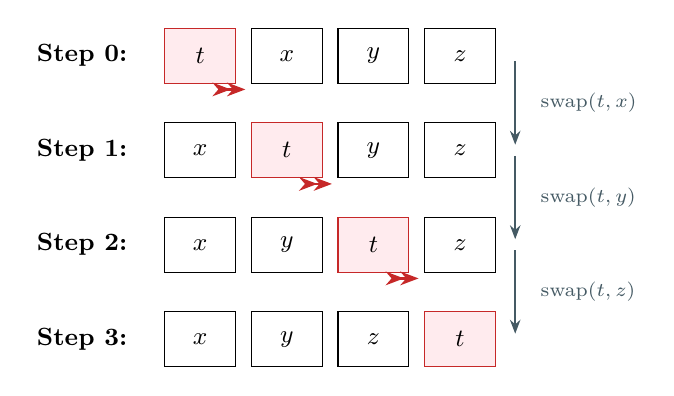
\begin{tikzpicture}[>=Stealth]
\def\xLabel{-1.5}   % x-position for step labels
\def\xBox{1.1}      % horizontal spacing between boxes
\def\yStart{2}       % y-position of first row
\def\yStep{1.2}      % vertical spacing between rows
\def\xTrans{4.0}     % x-position for transition arrows
\def\xTransLbl{4.2}  % x-position for transition labels

%% Nodes — each row: step index / t-position / labels left-to-right
\foreach \step/\tpos/\lblA/\lblB/\lblC/\lblD in {
  0/0/t/x/y/z,
  1/1/x/t/y/z,
  2/2/x/y/t/z,
  3/3/x/y/z/t%
} {
  \pgfmathsetmacro{\yrow}{\yStart - \step*\yStep}
  \node[font=\small\bfseries] at (\xLabel, \yrow) {Step \step:};
  \foreach \col/\lbl in {0/\lblA, 1/\lblB, 2/\lblC, 3/\lblD} {
    \pgfmathsetmacro{\xpos}{\col*\xBox}
    \ifnum\col=\tpos\relax
      \node[sortbox, fill=palRedLt, draw=palRed] (\lbl\step) at (\xpos, \yrow) {$\lbl$};
    \else
      \node[sortbox] (\lbl\step) at (\xpos, \yrow) {$\lbl$};
    \fi
  }
}

%% Swap Arrows (steps 0–2: t swaps with its right neighbour)
\foreach \step/\swapWith in {0/x, 1/y, 2/z} {
  \draw[stdarrow, palRed, <->] ([yshift=-2pt]t\step.south east) -- ([yshift=-2pt]\swapWith\step.south west);
}

%% Step Transition Arrows and Labels
\foreach \step/\partner in {0/x, 1/y, 2/z} {
  \pgfmathsetmacro{\yhi}{\yStart - \step*\yStep}
  \pgfmathsetmacro{\ylo}{\yStart - (\step+1)*\yStep}
  \pgfmathsetmacro{\ymid}{(\yhi+\ylo)/2}
  \draw[stdarrow, palGray] (\xTrans, \yhi) -- (\xTrans, \ylo);
  \node[font=\scriptsize, palGray, anchor=west] at (\xTransLbl, \ymid) {swap$(t,\partner)$};
}
\end{tikzpicture}
\caption{Bubble-sort swap illustration. Transaction $t$ (highlighted) does not conflict with $x$, $y$, or $z$, so iterated adjacent transpositions move $t$ to the end.}
\label{fig:bubble-sort}
\end{figure}

\begin{definition}[Respects Conflict Order]\label{def:respects-conflict}
$\mathit{respectsConflictOrder}(\mathit{order}, \mathit{hist}) \iff \forall t_1, t_2.\; \mathit{fullConflicts}(t_1, t_2) \wedge \mathit{before}(\mathit{hist}, t_1, t_2) \implies \mathit{before}(\mathit{order}, t_1, t_2)$
\end{definition}

\begin{definition}[Strong Core Serializability]\label{def:strong-serial}
$\mathit{strongCoreSerializable}(s_0, \mathit{hist}) \iff \forall \mathit{order}.\; \mathit{Perm}(\mathit{order}, \mathit{hist}) \wedge \mathit{respectsConflictOrder}(\mathit{order}, \mathit{hist}) \implies \mathit{applyCoreHistory}(s_0, \mathit{order}) = \mathit{applyCoreHistory}(s_0, \mathit{hist})$
\end{definition}

The definitions of $\mathit{respectsConflictOrder}$ and $\mathit{strongCoreSerializable}$ quantify over permutations of the history, which raises a natural question: are conflict-respecting permutations actually \emph{executable}? That is, if we applied the transactions in such a permutation, would each transaction find its required inputs available? The answer is yes, by construction of the conflict relation. If transaction~$B$ consumes an output produced by transaction~$A$, then $A.\mathit{outputs} \cap B.\mathit{inputs} \neq \emptyset$, so $\mathit{fullConflicts}(A, B)$ holds. Since $A$ was committed before $B$ in the original history, $\mathit{respectsConflictOrder}$ forces $A$ before $B$ in every considered permutation. More generally, every causal dependency between transactions is captured by a conflict edge, so no conflict-respecting permutation can place a transaction before the transaction it depends on.

\begin{theorem}[Acyclic Implies Strong Serializability]\label{thm:strong-serial}
\[
\mathit{hist.Nodup} \wedge \mathit{fullPrecGraphAcyclic}(\mathit{hist}) \implies \mathit{strongCoreSerializable}(s_0, \mathit{hist})
\]
\emph{(Mechanized: \texttt{acyclic\_strong\_serializable}, StarstreamPilot.lean.)}
\end{theorem}

\begin{proof}[Proof]
By strong induction on $|\mathit{hist}|$ using \texttt{List.reverseRecOn} (which decomposes the list by peeling the last element, aligning the Lean proof structure with the paper's ``bubble to end'' argument).

\emph{Base case} ($\mathit{hist} = []$): any permutation of $[]$ is $[]$; trivial.

\emph{Inductive case} ($\mathit{hist} = \mathit{init} \mathbin{+\!\!+} [t]$): given a conflict-respecting permutation $\mathit{order}$ of $\mathit{init} \mathbin{+\!\!+} [t]$:

\begin{enumerate}
  \item \textbf{Locate $t$}: since $t \in \mathit{order}$, write $\mathit{order} = \mathit{pre} \mathbin{+\!\!+} [t] \mathbin{+\!\!+} \mathit{suf}$.

  \item \textbf{Suffix is non-conflicting}: for each $x \in \mathit{suf}$, we have $\mathit{before}(\mathit{order}, t, x)$. If $\mathit{fullConflicts}(t, x)$ held, then by symmetry $\mathit{fullConflicts}(x, t)$, and since $x \in \mathit{init}$ we would have $\mathit{before}(\mathit{hist}, x, t)$, so $\mathit{respectsConflictOrder}$ would force $\mathit{before}(\mathit{order}, x, t)$---contradicting $\mathit{before}(\mathit{order}, t, x)$.

  \item \textbf{Bubble $t$ to end}: by \cref{lem:bubble-past}, $\mathit{ConflictEquiv}(\mathit{order}, \mathit{pre} \mathbin{+\!\!+} \mathit{suf} \mathbin{+\!\!+} [t])$.

  \item \textbf{Core state equivalence}: by \cref{thm:conflict-equiv-core}, $\mathit{applyCoreHistory}(s_0, \mathit{order}) = \mathit{applyCoreHistory}(s_0, \mathit{pre} \mathbin{+\!\!+} \mathit{suf} \mathbin{+\!\!+} [t])$.

  \item \textbf{Apply IH}: $\mathit{pre} \mathbin{+\!\!+} \mathit{suf}$ is a permutation of $\mathit{init}$ that respects its conflict order. By the induction hypothesis, $\mathit{applyCoreHistory}(s_0, \mathit{pre} \mathbin{+\!\!+} \mathit{suf}) = \mathit{applyCoreHistory}(s_0, \mathit{init})$.

  \item \textbf{Chain}: $\mathit{applyCoreHistory}(s_0, \mathit{order}) = \mathit{applyCoreHistory}(s_0, \mathit{init} \mathbin{+\!\!+} [t]) = \mathit{applyCoreHistory}(s_0, \mathit{hist})$.
\end{enumerate}
\end{proof}

\begin{corollary}[Strong Serializability from Ledger Invariant]\label{cor:serial-from-invariant}
$\mathit{ledgerInvariant}(L) \implies \mathit{strongCoreSerializable}(\mathit{coreOf}(L_0), L.\mathit{history})$.
\emph{(Mechanized: \texttt{acyclic\_precgraph\_strong\_serializable}.)}
\end{corollary}

The universal diamond property: the committed history's core state is an invariant of the conflict-order class. Any two conflict-respecting serializations produce identical UTxO and consumed sets. This result is precisely the confluence property from Mazurkiewicz trace theory~\cite{Mazurkiewicz1987}: the relation $\mathit{ConflictEquiv}$ (\cref{def:conflict-equiv}) is trace equivalence induced by the independence relation $\neg\,\mathit{fullConflicts}$, and \cref{thm:strong-serial} states that all traces in the same equivalence class produce the same core state. The ``diamond'' in ``universal diamond property'' is the same diamond as in Newman's lemma from abstract rewriting: if a single adjacent swap preserves the result (the local confluence step), then any finite sequence of swaps does too (global confluence). The mechanized proof makes this reasoning explicit through the inductive structure of $\mathit{ConflictEquiv}$.

The scope of the invariance is the \emph{core state}: the UTxO set and consumed set, which together determine asset ownership. This is the security-critical state. History ordering and auxiliary ledger fields (e.g., the ordered list of committed transactions, pending locks) may differ across conflict-respecting serializations, but the state that determines who owns what is invariant. For cross-shard consistency, this is the property that matters: different shards can apply non-conflicting transactions in different orders and still agree on asset ownership, without requiring a single global serialization.

Deployed systems rely on the same commutativity principle, albeit without formal proof. Solana's Sealevel runtime~\cite{Yakovenko2018} schedules non-conflicting account transactions in parallel across cores. Sui~\cite{Blackshear2023} bypasses consensus entirely for owned-object transactions, exploiting the fact that non-conflicting operations commute. Aptos Block-STM \cite{Gelashvili2023} uses optimistic parallel execution with abort-on-conflict, re-executing only when a conflict is detected. All three designs implicitly assume what Core Commutativity (\cref{thm:core-commute}) formalizes. The mechanized proof in this section provides the missing formal justification for the commutativity assumption that underlies these systems.

%% ═══════════════════════════════════════════════════════════════════════════
\section{MPST-to-Ledger Bridge}\label{sec:bridge}

The preceding sections developed two formal layers independently. The MPST coordination layer (\cref{sec:model}) defines global scripts, event structures, role projections, and local conformance---the machinery for specifying and checking multiparty protocols. The ledger commit layer (\cref{sec:opsem}) defines the operational semantics, commit guards, invariant preservation, and the conflict serializability results of \cref{sec:serializability}. The bridge problem is to connect these layers: to show that a transaction that commits on the ledger actually followed the prescribed multiparty protocol (soundness), and that any protocol-compliant execution can lead to a valid commit (completeness). Without this connection, the two layers would be independent formalisms---the MPST types would guarantee protocol structure but say nothing about ledger state, and the ledger invariants would guarantee asset safety but say nothing about whether the protocol was followed.

The bridge has three parts, corresponding to the three subsections. First, \emph{trace consistency} (\cref{sec:trace-consistency}) identifies conditions under which shard-local verification---checking each role's projected trace independently---can reconstruct the global trace consistency needed for commit. This reduces a global property (the entire multiparty trace is valid) to a conjunction of local properties (each role's projection conforms) plus lightweight cross-role conditions. Second, \emph{coordination witnesses} (\cref{sec:coordination-witness}) connect these trace-level results to the ledger's commit mechanism: the bidirectional witness theorems show that a coordination witness is globally valid if and only if it passes all shard-local checks, and the coordinated commit theorem shows that the global commit guard implies all local commit guards. Third, \emph{concurrent-to-serial refinement} (\cref{sec:refinement}) shows that the concurrent ledger execution---with its interleavings of effect handling, lock acquisition, and coroutine scheduling---refines a serial specification where transactions commit one at a time.

The refinement proof follows the classical stuttering simulation approach: an abstraction map projects the concrete ledger state onto a serial specification state, concrete steps that only modify concurrency-control metadata are classified as stuttering (invisible to the specification), and each concrete commit step is shown to correspond to exactly one serial step. This technique is standard in distributed systems verification---Lamport's TLA~\cite{Lamport1994} formalizes stuttering refinement for state machines, and IronFleet~\cite{Hawblitzel2015} and Verdi~\cite{Wilcox2015} use similar simulation proofs to connect protocol specifications to implementation code. The novelty here is combining stuttering simulation with MPST-based protocol verification: the refinement witness for each commit step includes not just ledger-level validity (inputs live, outputs fresh, no double-spend) but also a cryptographic attestation that the multiparty protocol was correctly executed.

\subsection{Trace Consistency and Cross-Role Reconstruction}\label{sec:trace-consistency}

A central question is: can shard-local verification (checking each role's local trace) reconstruct the global trace consistency needed for commit?

\begin{definition}[Before]\label{def:before}
$\mathit{Before}(\mathit{tr}, a, b) \iff \exists \ell_1, \ell_2.\; \mathit{tr} = \ell_1 \mathbin{+\!\!+} [a] \mathbin{+\!\!+} \ell_2 \wedge b \in \ell_2$.
\end{definition}

\begin{definition}[Trace Consistency]\label{def:trace-consistency}
A trace $\mathit{tr}$ is \emph{consistent} with script $S$, written $S.\mathit{traceConsistent}(\mathit{tr})$, if:
\begin{enumerate}
  \item $\mathit{tr}$ is duplicate-free ($\mathit{tr.Nodup}$)
  \item All events in $\mathit{tr}$ are in $S.\mathit{events}$
  \item No event in $\mathit{tr}$ conflicts with any other event in $\mathit{tr}$
  \item For every order edge $e' < e$ with $e \in \mathit{tr}$, $\mathit{Before}(\mathit{tr}, e', e)$
\end{enumerate}
\end{definition}

These four conditions are the standard requirements for a \emph{configuration} of an event structure~\cite{Winskel1986}: no duplicates (each event occurs at most once), membership in the event set (only events from the script), conflict-freedom (no two mutually exclusive events co-occur), and causal closure (if an event is included, all its causal predecessors are included in the correct order). A trace satisfying these conditions is a linearization of such a configuration---it represents an executable prefix of the protocol in which every event finds its prerequisites already completed. The distinction between $\mathit{traceConsistent}$ and $\mathit{validTrace}$ (\cref{thm:consistent-valid}) is that the former is a static structural check on a list of events, while the latter asserts that the trace can be produced by the operational semantics of the event structure. \Cref{thm:consistent-valid} proves these coincide: the structural conditions are exactly the enablement conditions, so checking a trace against \cref{def:trace-consistency} is equivalent to replaying it step by step against the event-structure semantics.

\begin{definition}[Cross-Role Consistency]\label{def:cross-role}
A trace is \emph{cross-role consistent} if:
\begin{enumerate}
  \item Events with disjoint role sets do not conflict: $\mathit{disjointRoles}(e, f) \implies \neg(e \mathbin{\#} f)$.
  \item Order between disjoint-role events is witnessed: $\mathit{disjointRoles}(e', e) \wedge e' < e \wedge e \in \mathit{tr} \implies \mathit{Before}(\mathit{tr}, e', e)$.
\end{enumerate}
\end{definition}

Local conformance per role ($\mathit{localConform}$) ensures that each participant follows its own projected protocol---events involving role~$r$ appear in the correct order and without intra-role conflicts. But local conformance says nothing about the relationship between events on disjoint roles: if event~$e$ involves only role~$r_1$ and event~$f$ involves only role~$r_2$, no single role's projection sees both. Cross-role consistency (\cref{def:cross-role}) fills this gap. Condition~(1) requires that events on independent roles do not conflict---a property guaranteed when roles access disjoint UTxO sets (as established by the role-separation results in \cref{sec:sbac-integration}), but stated here as an explicit proof obligation. Condition~(2) ensures that any causal ordering the global protocol imposes between events on different roles is respected in the trace, even though no single role observes both events. Together with the four conditions of \cref{def:trace-consistency}, these requirements exactly characterize the linearizations of conflict-free, causally-closed configurations in the event structure induced by the global script, in the sense of Winskel's event-structure semantics~\cite{Winskel1986}. The case split in the proof of \cref{thm:local-cross-global}---shared role vs.\ disjoint roles---mirrors this decomposition: intra-role properties come from local conformance, and inter-role properties come from cross-role consistency.

\begin{theorem}[Local + Cross-Role $\Rightarrow$ Global Consistency]\label{thm:local-cross-global}
\begin{align*}
&\mathit{WF}(S) \wedge \mathit{tr.Nodup} \wedge (\forall r \in S.\mathit{roles}.\; \mathit{localConform}(S, r, \mathit{traceProj}(S, r, \mathit{tr}))) \\
&\quad \wedge \mathit{crossRoleConsistent}(S, \mathit{tr}) \implies S.\mathit{traceConsistent}(\mathit{tr})
\end{align*}
\emph{(Mechanized: \texttt{traceConsistent\_of\_local\_and\_cross}, Script.lean.)}
\end{theorem}

\begin{proof}[Proof sketch]
For \emph{conflict-freedom}: given events $a, b$ in $\mathit{tr}$, either they share a role or have disjoint roles. If disjoint, cross-role consistency directly gives $\neg(a \mathbin{\#} b)$. If they share a role $r$, then both appear in $\mathit{traceProj}(S, r, \mathit{tr})$; local conformance implies the local trace is conflict-free, which lifts to the global level.

For \emph{order-respect}: given $e' < e$ with $e \in \mathit{tr}$, case-split on whether $e'$ and $e$ share a role. If disjoint, cross-role consistency provides $\mathit{Before}(\mathit{tr}, e', e)$. If shared via role $r$, local trace validity ensures $e'$ appears before $e$ in the projected trace, which lifts to the global trace via \texttt{before\_of\_filter}.
\end{proof}

\begin{theorem}[Consistent Implies Valid Trace]\label{thm:consistent-valid}
$S.\mathit{traceConsistent}(\mathit{tr}) \implies S.\mathit{validTrace}(\mathit{tr})$.
\emph{(Mechanized: \texttt{traceConsistent\_implies\_validTrace}.)}
\end{theorem}

\begin{proof}[Proof sketch]
By induction on $\mathit{tr}$, converting consistency evidence into enablement at each step: predecessors present (from order-respect), no conflicts (from pairwise conflict-freedom), event membership (from events check).
\end{proof}

Together, \cref{thm:local-cross-global,thm:consistent-valid} establish a two-step reduction. \Cref{thm:local-cross-global} reduces global trace consistency---a property of the entire multiparty execution---to a conjunction of per-role local conformance checks and cross-role consistency conditions. \Cref{thm:consistent-valid} then shows that any globally consistent trace is a valid execution of the event structure, meaning it could have been produced by the MPST operational semantics. The practical consequence is that a shard hosting role~$r$ needs to check only that $r$'s projected trace conforms locally; the cross-role conditions are enforced by the coordination witness construction (which embeds the global trace) and the cryptographic proof (which attests to the trace's consistency). This decomposition is what makes shard-local verification feasible: without it, every shard would need to replay the entire multiparty execution to decide whether to commit.

\subsection{Coordination Witness and Commit}\label{sec:coordination-witness}

The S-BAC (Sharded Byzantine Atomic Commit) bridge layer connects the MPST coordination results from the previous subsection to the ledger's commit mechanism. A coordination witness $W = (S, \mathit{tr})$ pairs a global script with a trace attesting to protocol compliance. The question is whether checking this witness can be decomposed across shards: does global validity of the witness imply that each shard's local check will pass, and conversely does passing all local checks imply global validity? The following two theorems answer both directions affirmatively.

\begin{theorem}[Bidirectional Witness Theorems]\label{thm:bidirectional}
\begin{enumerate}
  \item \emph{Top-down}: $\mathit{witnessGlobalOK}(W) \implies \mathit{witnessLocalOK}(W)$. A globally valid witness can be verified shard-locally.
  \item \emph{Bottom-up}: $\mathit{WF}(W.\mathit{script}) \wedge \mathit{witnessConsistent}(W) \implies \mathit{witnessGlobalOK}(W)$. If the witness trace is consistent, global conformance follows.
\end{enumerate}
\end{theorem}

\begin{theorem}[Coordinated Commit Implies Local Commit]\label{thm:coord-local}
$\mathit{coordCommitEnabled}(m, L, \mathit{ctx}) \implies \mathit{coordCommitEnabledLocal}(m, L, \mathit{ctx})$.
\emph{(Mechanized: \texttt{coordCommitEnabledLocal\_of\_global}.)}
\end{theorem}

\paragraph{Cross-shard deadlock.} The S-BAC protocol is deadlock-free by construction: each transaction is submitted to all relevant shards simultaneously during prepare, and shards respond independently. There is no circular wait because shards do not hold resources across transactions---a shard either prepares or aborts, and the final decision is made by the coordinator after collecting all responses. This argument depends on three premises: (1)~the S-BAC prepare phase has bounded duration (enforced by timeout), (2)~the abort constructor unconditionally releases locks (\cref{def:ledger}), and (3)~the S-BAC coordination protocol is itself deadlock-free under partial synchrony.

The bidirectional witness theorems (\cref{thm:bidirectional}) establish that global protocol validity and shard-local validity are equivalent, given well-formedness and trace consistency. The top-down direction guarantees that a globally valid witness will pass every shard's local checks---no honest shard will reject a legitimate transaction. The bottom-up direction guarantees the converse: if every shard independently approves its roles' projections and the trace is consistent, then the global protocol was followed. Together, these two directions justify the decentralized verification architecture: no single authority needs to check the global protocol end-to-end. Each shard verifies only the roles it hosts, and the trace consistency conditions (\cref{def:trace-consistency,def:cross-role}) ensure that these local checks compose into a global guarantee. This decomposition is critical for scalability---global protocol checking would require every shard to see every event, defeating the purpose of sharding.

\Cref{thm:coord-local} extends this result to the commit layer: if the full coordinated commit guard passes (combining both ledger-level validity and witness-level protocol compliance), then every shard's local commit condition is satisfied. This means the S-BAC prepare phase will succeed on all honest shards---no shard will unilaterally abort a transaction that the global commit guard has approved. The converse direction (all-local-approve implies global-approve) follows from the bottom-up witness theorem combined with the structure of $\mathit{coordCommitEnabled}$: if every shard's local ledger checks and local witness checks pass, and the trace is consistent, then both $\mathit{commitEnabledStrong}$ and $\mathit{witnessGlobalOK}$ hold, satisfying the global guard.

\subsection{Concurrent-to-Serial Refinement}\label{sec:refinement}

We prove that the concurrent ICE-UTxO semantics refines a serial specification where transactions commit atomically one at a time.

\begin{definition}[Serial Step]\label{def:serial-step}
A serial step atomically commits a proof-verified, valid transaction:
\[
\mathit{SerialStep}(m, L, L') \iff \exists \mathit{tx}.\; \mathit{allProofsVerified}(\mathit{tx}) \wedge \mathit{validTx}(L, \mathit{tx}) \wedge \mathit{tx.phase} = \text{Committing} \wedge L' = \mathit{applyCommit}(L, \mathit{tx})
\]
\end{definition}

\begin{definition}[Stuttering]\label{def:stuttering}
A step is \emph{stuttering} if $\mathit{absLedger}(L) = \mathit{absLedger}(L')$. Stuttering steps change only the concurrency-control fields without modifying the core UTxO/consumed/history state.
\end{definition}

\begin{definition}[Abstraction Map]\label{def:abstraction-map}
$\mathit{absLedger}(L) = L[\mathit{locked} := \emptyset, \mathit{pending} := \emptyset, \mathit{effects} := \lambda\_.\, [], \mathit{handlerStacks} := \lambda\_.\, []]$.
\end{definition}

The abstraction map erases exactly the concurrency-control fields that exist only in the concurrent implementation: $\mathit{locked}$ tracks which UTxOs are reserved during the S-BAC prepare phase (preventing double-spending during coordination), $\mathit{pending}$ tracks transactions that have been submitted but not yet committed or aborted, and $\mathit{effects}$ and $\mathit{handlerStacks}$ manage the algebraic-effect coroutine machinery that allows transactions to yield, raise effects, and resume. None of these fields exist in the serial specification, where each transaction commits instantaneously in a single atomic step. The result is that $\mathit{absLedger}(L)$ retains only the UTxO set, the consumed set, and the committed history---the state components that determine asset ownership and transaction ordering, and the only components that the serial specification tracks.

\begin{theorem}[Concurrent Refines Serial]\label{thm:concurrent-refines-serial}
\[
\mathit{Steps}(m, L_0, L_n) \wedge \mathit{ledgerInvariant}(L_0) \implies \mathit{SerialSteps}(m, \mathit{absLedger}(L_0), \mathit{absLedger}(L_n))
\]
\emph{(Mechanized: \texttt{concurrent\_refines\_serial}, StarstreamPilot.lean.)}
\end{theorem}

\begin{proof}[Proof sketch]
By induction on the \texttt{Steps} derivation. At each step, apply \texttt{step\_preserves\_invariant} to maintain the invariant for the induction hypothesis. Then case-split on the step constructor:
\begin{itemize}
  \item \textbf{Stuttering cases} (7 of 8): \texttt{addPending}, \texttt{lockInputs}, \texttt{abort}, \texttt{installH}, \texttt{uninstallH}, \texttt{raiseE}, \texttt{handleE}. Each has a dedicated lemma showing $\mathit{absLedger}(L) = \mathit{absLedger}(L')$. The serial trace is unchanged.
  \item \textbf{Visible case} (1 of 8): \texttt{commit}. The commit step produces a \texttt{SerialStep} in the abstract trace, constructed from the commit preconditions.
\end{itemize}
\end{proof}

The practical consequence is that the concurrent ledger---with its interleavings of effect handling, lock acquisition, and coroutine scheduling---is an implementation detail. Any concurrent execution simplifies to an equivalent serial execution where transactions commit one at a time. Reasoning about ICE-UTxO's correctness thus reduces to reasoning about sequential commits, which is substantially simpler.

The 7-to-1 split between stuttering and visible steps reflects a design principle: the abstraction map $\mathit{absLedger}$ (\cref{def:abstraction-map}) erases exactly the fields that manage concurrency control---locks, pending transactions, effect queues, and handler stacks. The seven non-commit constructors manipulate only these fields; none modify the UTxO set, consumed set, or committed history. Only the $\mathit{commit}$ step changes the core state visible to the serial specification.

This decomposition is the standard structure of a stuttering simulation in the sense of Lamport~\cite{Lamport1994}: the implementation takes many ``internal'' steps for each ``visible'' step of the specification. A transaction may raise and handle arbitrarily many effects, install and uninstall multiple handlers, and retry after aborts---an unbounded number of concrete steps---before it eventually commits. The proof does not require a bound on this ratio; it requires only that each concrete step either maps to a serial step (the commit case) or leaves the abstract state unchanged (the stuttering case). The liveness results from \cref{sec:liveness} ensure that this stuttering does not continue forever: under fair scheduling, every pending transaction eventually commits or aborts, so the concrete execution cannot stutter indefinitely without making abstract progress.

\begin{figure}[t]
\centering
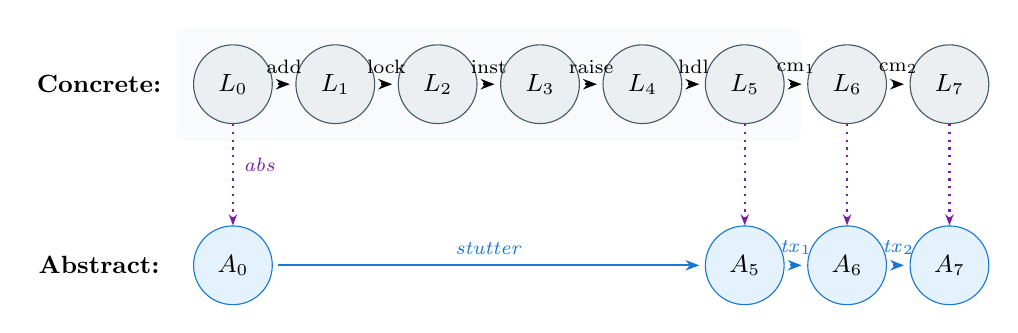
\begin{tikzpicture}[
  cstate/.style={draw, circle, minimum size=1.0cm, font=\small, fill=palGrayLt, draw=palGray},
  astate/.style={draw, circle, minimum size=1.0cm, font=\small, fill=palBlueLt, draw=palBlue},
  >=Stealth,
  node distance=1.2cm
]
\def\yConcrete{1.5}    % y-position for concrete row
\def\yAbstract{-0.8}   % y-position for abstract row
\def\xSpacing{1.3}     % horizontal spacing between concrete states

%% Concrete Row
\node[font=\small\bfseries] at (-1.7, \yConcrete) {Concrete:};
\foreach \i/\lbl in {0/L_0, 1/L_1, 2/L_2, 3/L_3, 4/L_4, 5/L_5, 6/L_6, 7/L_7} {
  \node[cstate] (c\i) at (\i*\xSpacing, \yConcrete) {$\lbl$};
}

%% Concrete Edges
\foreach \i/\j/\lbl in {0/1/add,1/2/lock,2/3/inst,3/4/raise,4/5/hdl,5/6/cm$_1$,6/7/cm$_2$} {
  \draw[stdarrow] (c\i) -- node[above, font=\scriptsize] {\lbl} (c\j);
}

%% Stuttering Background
\begin{scope}[on background layer]
  \node[rounded corners, fill=palGrayLt!30, fit=(c0)(c5), inner sep=6pt] {};
\end{scope}

%% Abstract Row — aligned to concrete node x-positions
\node[font=\small\bfseries] at (-1.7, \yAbstract) {Abstract:};
\node[astate] (a0) at (c0 |- 0,\yAbstract) {$A_0$};
\node[astate] (a5) at (c5 |- 0,\yAbstract) {$A_5$};
\node[astate] (a6) at (c6 |- 0,\yAbstract) {$A_6$};
\node[astate] (a7) at (c7 |- 0,\yAbstract) {$A_7$};

%% Abstract Edges
\draw[stdarrow, palBlue] (a0) -- node[above, font=\scriptsize] {$\mathit{stutter}$} (a5);
\draw[stdarrow, palBlue] (a5) -- node[above, font=\scriptsize] {$\mathit{tx}_1$} (a6);
\draw[stdarrow, palBlue] (a6) -- node[above, font=\scriptsize] {$\mathit{tx}_2$} (a7);

%% Abstraction Map
\draw[stutterarrow, palPurple] (c0) -- node[right, font=\scriptsize, pos=0.4] {$\mathit{abs}$} (a0);
\draw[stutterarrow, palPurple] (c5) -- (a5);
\draw[stutterarrow, palPurple] (c6) -- (a6);
\draw[stutterarrow, palPurple] (c7) -- (a7);
\end{tikzpicture}
\caption{Refinement diagram: concrete concurrent steps map to abstract serial steps via $\mathit{absLedger}$. Non-commit steps are stuttering.}
\label{fig:refinement}
\end{figure}

The predicate $\mathit{refinementWitness}(m, L, \mathit{tx})$ bundles the conditions under which a concrete commit step corresponds to an abstract serial step. Specifically, it requires: (a)~the transaction's coordination witness is globally valid ($\mathit{witnessGlobalOK}$), certifying that the MPST protocol was followed; (b)~all cryptographic proof commitments have been verified ($\mathit{allProofsVerified}(\mathit{tx})$); (c)~the transaction is structurally valid in the current ledger state ($\mathit{validTx}(L, \mathit{tx})$)---inputs are live, outputs are fresh, and inputs and outputs are disjoint; and (d)~the transaction is in the $\text{Committing}$ phase. This is essentially $\mathit{coordCommitEnabled}$ (\cref{sec:sbac-integration}) restricted to a single transaction in a given ledger state. The name ``circuit witness'' reflects the deployment architecture: in practice, MPST trace compliance is attested by an IVC/SNARK proof (the ``circuit''), so verifying the $\mathit{refinementWitness}$ amounts to checking one cryptographic proof rather than replaying the entire multiparty protocol execution.

\begin{theorem}[Circuit Witness Implies Serial Step]\label{thm:circuit-serial}
$\mathit{refinementWitness}(m, L, \mathit{tx}) \implies \mathit{SerialStep}(m, L, \mathit{applyCommit}(L, \mathit{tx}))$.
\emph{(Mechanized: \texttt{circuit\_witness\_implies\_serial\_step}.)}
\end{theorem}

The results of this section establish a layered correctness argument for the ICE-UTxO system. Trace consistency (\cref{def:trace-consistency,def:cross-role}) and the bidirectional witness theorems (\cref{thm:bidirectional}) ensure that shard-local verification is both sound and complete with respect to the global MPST protocol: a transaction commits only if its coordination witness certifies a protocol-compliant execution, and every protocol-compliant execution produces a witness that passes shard-local checks. The concurrent-to-serial refinement (\cref{thm:concurrent-refines-serial}) then shows that the committed transactions, viewed through the abstraction map, form a serial history---each transaction appears to execute atomically and in isolation. Combined with the conflict serializability result from \cref{sec:serializability}, this gives a two-level guarantee: the committed history is serializable (\cref{sec:serializability}), and each transaction in that history faithfully implements its declared multiparty protocol (this section).

The two-layer architecture mirrors the approach of verified distributed systems such as IronFleet~\cite{Hawblitzel2015} and Verdi~\cite{Wilcox2015}. In IronFleet, a high-level protocol specification (e.g., a Paxos state machine) is connected to a low-level implementation via a simulation proof; in Verdi, verified system transformers lift correctness from idealized models to realistic network settings. Here, the MPST event-structure semantics serves as the protocol specification layer, and the concrete UTxO operational semantics serves as the implementation layer. \Cref{thm:concurrent-refines-serial} is the simulation theorem connecting them. The key difference is that ICE-UTxO uses cryptographic proof-carrying data to certify protocol compliance at commit time, rather than relying on runtime message monitoring. This shifts the trust boundary: instead of trusting that each participant runs correct code (as in IronFleet), the ledger verifies a cryptographic attestation that the protocol was followed, regardless of how participants behaved internally.

The bridge relies on assumptions stated in \cref{sec:commit-rule}: (i)~ZK verifier soundness---the external ZK verification oracle is assumed to be sound, so that a \texttt{Verified} flag genuinely corresponds to a valid proof of protocol compliance; (ii)~S-BAC shard honesty---the cross-shard atomic commit protocol assumes fewer than one-third Byzantine validators per shard, consistent with the Chainspace fault model~\cite{AlBassam2018}; and (iii)~well-formedness of the global script ($\mathit{WF}(S)$), which is a checkable structural condition on the MPST global type. The S-BAC protocol itself is not mechanized in Lean; its correctness is assumed from the established literature on Byzantine atomic commit~\cite{AlBassam2018}. Formally verifying the S-BAC layer---perhaps using a framework like Verdi's verified system transformers---would close this remaining gap between the mechanized proofs and a deployed system.

%% ═══════════════════════════════════════════════════════════════════════════
\section{Formal Verification}\label{sec:mechanization}

The ICE-UTxO model is verified through two complementary formal artifacts: a Lean~4 mechanization that proves safety properties universally, and a TLA+ specification that validates liveness properties by model checking under fairness assumptions. Neither artifact alone covers the full verification space; together, they do.

\subsection{Dual Verification Strategy}\label{sec:dual-strategy}

Safety properties --- no double-spend, serializable histories, proof-gated commit --- guarantee that the system never enters an invalid state. But a ledger that commits nothing satisfies all of them. The serializability theorem guarantees that \emph{if} transactions commit, their ordering is consistent; it says nothing about whether any transaction \emph{ever} commits. A system that silently deadlocks is safe by every Lean theorem in this paper.

This is not a theoretical concern. ICE-UTxO introduces three mechanisms that create liveness risks absent from vanilla eUTxO. First, \emph{locks create starvation risk}: in pessimistic mode, \texttt{lockInputs} acquires exclusive locks on input UTxOs; if a transaction stalls --- because proof generation fails or a counterparty disappears --- those UTxOs are unavailable to every other transaction, and without guaranteed eventual abort, lock starvation cascades through the system. Second, \emph{effect queues create coroutine deadlock risk}: when a coroutine raises an effect, it enters \texttt{Suspended\_at\_Effect} and cannot proceed until a handler processes the effect; if effect handling stalls, the originating transaction can never reach the committing phase. Third, \emph{cross-shard coordination creates progress risk}: S-BAC requires all involved shards to reach consensus; if any shard's BFT consensus stalls, the entire multi-shard transaction blocks.

The division of labor between the two artifacts reflects a fundamental limitation in each tool's logic. Lean's dependent type theory can express universally quantified properties over all states and all transitions (``for every step, the invariant is preserved''), but it cannot express temporal operators: $\Box$ (always), $\Diamond$ (eventually), and fairness ($\mathit{WF}$, $\mathit{SF}$) are outside the logic. TLA+'s temporal logic expresses liveness properties naturally (``under $\mathit{WF}(\text{commit})$, a continuously enabled transaction eventually commits''), but its model checker can only validate them on bounded instances, not prove them for all executions.

The relationship between the artifacts is symbiotic. Each TLA+ liveness property depends on a specific Lean safety lemma: Lean proves that the \emph{enabling conditions} exist (the commit step is available, abort is always possible, effect handling decreases the queue); TLA+ validates that fair scheduling eventually \emph{exploits} those conditions. The Lean proofs without TLA+ leave open whether the system ever makes progress; the TLA+ properties without Lean lack the supporting safety guarantees on which they depend.

\subsection{Lean Proof Architecture}\label{sec:mech-architecture}

The Lean~4 mechanization proves three main results: (1)~a six-part safety invariant is preserved by every state transition; (2)~committed transaction histories are conflict-serializable; and (3)~the concurrent execution refines a serial specification where transactions commit one at a time. A bridge layer connects these ledger-level results to the MPST coordination layer, proving that protocol compliance decomposes into shard-local checks. Every proof is fully discharged --- no \texttt{sorry}, \texttt{admit}, or \texttt{axiom} --- and the only classical reasoning is a single decidable case split on finite role sets.

The development follows a two-track architecture. Track~1 (Ledger) reasons about UTxO state, conflicts, and serializability; Track~2 (Coordination) reasons about event structures, projections, and protocol compliance. The two tracks share a narrow interface --- the $\mathit{coordCommitEnabled}$ predicate --- which conjoins both tracks' preconditions into a single commit guard.

\subsection{Proof Architecture}\label{sec:mech-architecture}

The mechanization is split into two tracks connected by a bridge. This is not a code-organization convenience --- it reflects a fundamental separation between two proof domains that share a narrow interface.

\paragraph{Track~1 (Ledger).}
Track~1 reasons about UTxO sets, conflicts, invariants, and serializability. Its central objects are: \texttt{Step} (an inductive with eight constructors, one per state transition: \texttt{addPending}, \texttt{lockInputs}, \texttt{commit}, \texttt{abort}, \texttt{installH}, \texttt{uninstallH}, \texttt{raiseE}, \texttt{handleE}); $\mathit{ledgerInvariant}$ (a six-part safety predicate preserved by every step); $\mathit{CoreState}$ (the abstraction that makes commutativity provable); and $\mathit{absLedger}$ (the refinement map that drops concurrency-control fields). The key design insight is a double abstraction: $\mathit{CoreState}$ drops history so that applying transactions in different orders \emph{can} produce equal states (enabling the serializability proof), while $\mathit{absLedger}$ drops pending, locked, effects, and handler stacks so that non-commit steps \emph{do} produce equal states (enabling the stuttering simulation).

\paragraph{Track~2 (Coordination).}
Track~2 reasons about event structures, projections, traces, and protocol compliance. Its central objects are: \texttt{Script} (an event structure with partial order and conflict relation); \texttt{LocalScript} (per-role projection); \texttt{Program} (PTB commands with four dependency relations --- data, ordering, UTxO, and interface --- that combine into $\mathit{orderRel}$ and $\mathit{conflictRel}$); and \texttt{CoordWitness} (a script--trace pair attesting to protocol compliance). The key insight is that global trace consistency decomposes into per-role local conformance plus cross-role consistency, which is what makes shard-local verification possible without replaying the entire multiparty execution.

\paragraph{The bridge.}
The two tracks meet at the predicate $\mathit{coordCommitEnabled}$, which conjoins $\mathit{commitEnabledStrong}$ (the ledger-track guard: proof verified, inputs live, outputs fresh, phase is committing, not in history) and $\mathit{witnessGlobalOK}$ (the coordination-track guard: the trace globally conforms to the script). This is the sole point where both proof domains interact. The bridge theorems then show this conjunction decomposes to shard-local checks: each shard verifies only the roles it hosts and the UTxOs it manages, and these independent checks compose into the global guarantee.

\paragraph{The Oracle subtrack.}
An independent executable model (\texttt{Starstream/Oracle/*.lean}) maintains its own type universe with \texttt{Bool}-valued predicates and gas metering. Its four-phase proof decomposition (Phases~A--D) verifies transaction validation from input checking through batch processing. The PhaseD bridge theorems lift key Starstream properties (\texttt{commit\_preserves\_no\_double\_spend}, \texttt{step\_preserves\_invariant}, \texttt{concurrent\_refines\_serial}, among others) to the Oracle namespace, each requiring only a single \texttt{simpa~using} tactic --- confirming that the executable model adds no new proof obligations to the core theory.

\begin{figure}[t]
\centering
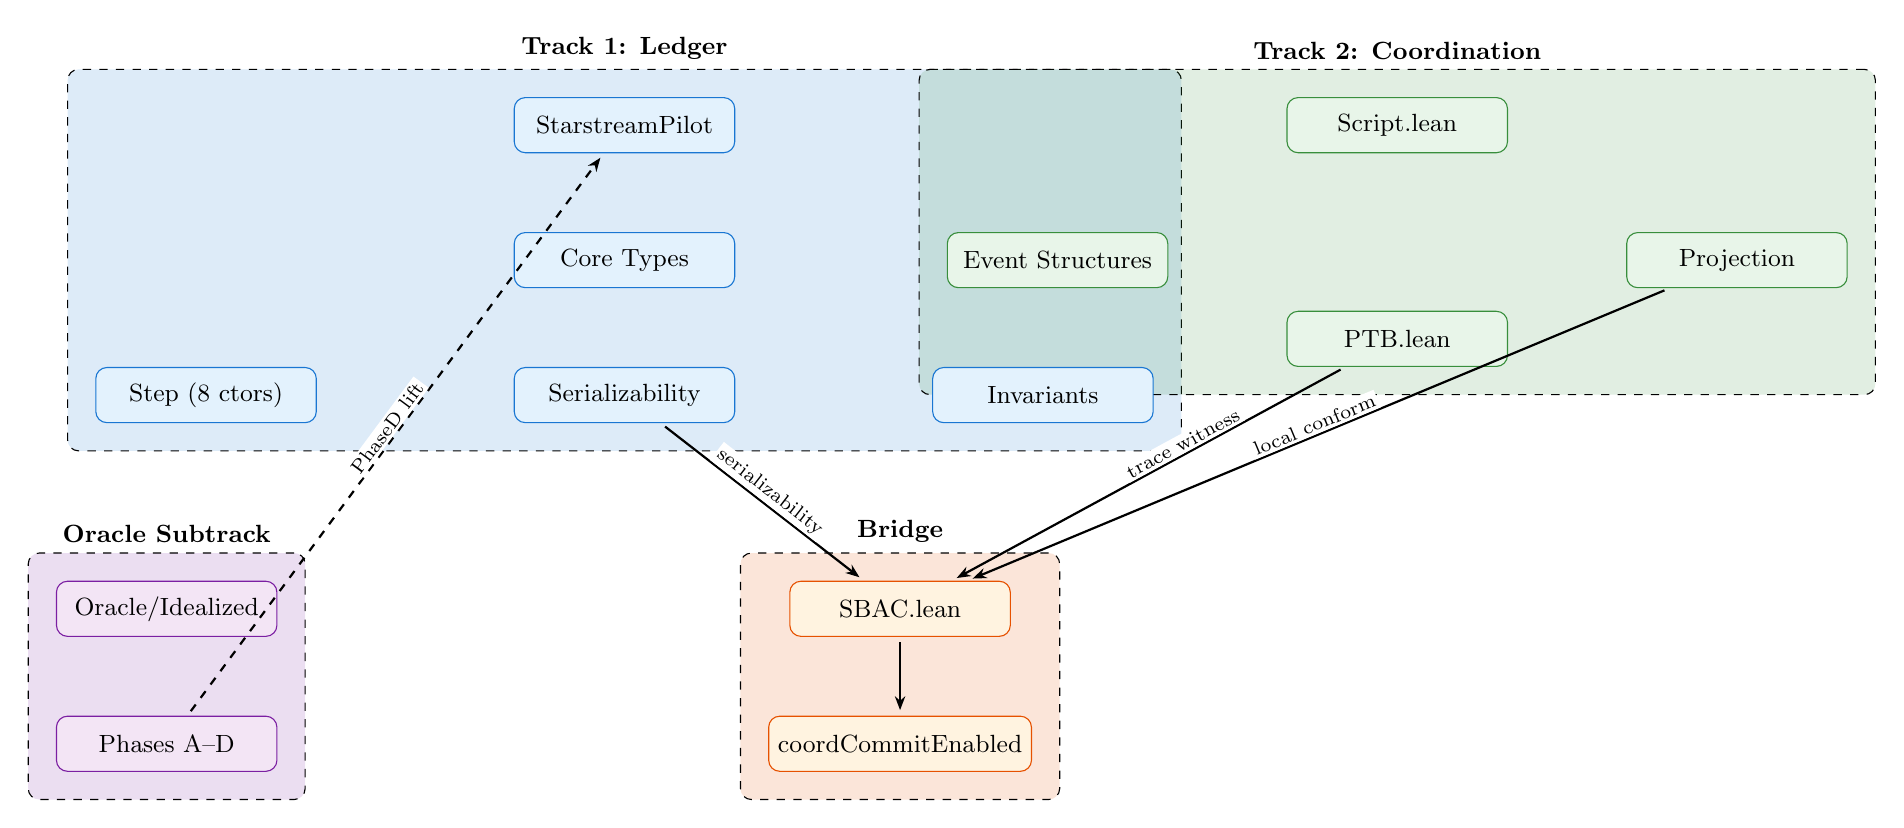
\begin{tikzpicture}[
  mnode/.style={modnode, minimum width=2.8cm},
  >=Stealth,
  node distance=1.0cm
]
%% Track 1: Ledger
\node[mnode, fill=palBlueLt, draw=palBlue] (ssp) {StarstreamPilot};
\node[mnode, fill=palBlueLt, draw=palBlue, below=of ssp] (core) {Core Types};
\node[mnode, fill=palBlueLt, draw=palBlue, below left=1.0cm and 2.5cm of core] (step) {Step (8 ctors)};
\node[mnode, fill=palBlueLt, draw=palBlue, below=of core] (serial) {Serializability};
\node[mnode, fill=palBlueLt, draw=palBlue, below right=1.0cm and 2.5cm of core] (inv) {Invariants};
\begin{scope}[on background layer]
  \node[trackgroup, fill=palBlue, label={[font=\small\bfseries]above:Track 1: Ledger}]
    (t1bg) [fit=(ssp)(core)(step)(serial)(inv)] {};
\end{scope}

%% Track 2: Coordination
\node[mnode, fill=palGreenLt, draw=palGreen, right=7.0cm of ssp] (script) {Script.lean};
\node[mnode, fill=palGreenLt, draw=palGreen, below left=1.0cm and 1.5cm of script] (es) {Event Structures};
\node[mnode, fill=palGreenLt, draw=palGreen, below right=1.0cm and 1.5cm of script] (proj) {Projection};
\node[mnode, fill=palGreenLt, draw=palGreen, below=2.0cm of script] (ptb) {PTB.lean};
\begin{scope}[on background layer]
  \node[trackgroup, fill=palGreen, label={[font=\small\bfseries]above:Track 2: Coordination}]
    [fit=(script)(es)(proj)(ptb)] {};
\end{scope}

%% Bridge
\node[mnode, fill=palOrangeLt, draw=palOrange, below=2.0cm of serial, xshift=3.5cm] (sbac) {SBAC.lean};
\node[mnode, fill=palOrangeLt, draw=palOrange, minimum width=3.2cm, below=of sbac] (coord) {coordCommitEnabled};
\begin{scope}[on background layer]
  \node[trackgroup, fill=palOrange, label={[font=\small\bfseries]above:Bridge}]
    [fit=(sbac)(coord)] {};
\end{scope}

%% Oracle Subtrack
\node[mnode, fill=palPurpleLt, draw=palPurple, below=2.0cm of step, xshift=-0.5cm] (oracle) {Oracle/Idealized};
\node[mnode, fill=palPurpleLt, draw=palPurple, below=of oracle] (phases) {Phases A--D};
\begin{scope}[on background layer]
  \node[trackgroup, fill=palPurple, label={[font=\small\bfseries]above:Oracle Subtrack}]
    [fit=(oracle)(phases)] {};
\end{scope}

%% Dependency Edges
\draw[stdarrow] (serial) -- node[above, font=\scriptsize, sloped, fill=white, inner sep=1pt] {serializability} (sbac);
\draw[stdarrow] (ptb) -- node[above, font=\scriptsize, sloped, fill=white, inner sep=1pt, pos=0.4] {trace witness} (sbac);
\draw[stdarrow] (proj) -- node[above, font=\scriptsize, sloped, fill=white, inner sep=1pt] {local conform} (sbac);
\draw[stdarrow] (sbac) -- (coord);
\draw[stdarrow, dashed] (phases) -- (ssp) node[midway, above, font=\scriptsize, sloped, fill=white, inner sep=1pt] {PhaseD lift};
\end{tikzpicture}
\caption{Proof architecture of the Lean mechanization. The two tracks meet at $\mathit{coordCommitEnabled}$ through the SBAC bridge. The Oracle subtrack connects back to Track~1 via PhaseD bridge theorems.}
\label{fig:module-deps}
\end{figure}

\subsection{What Is Proved}\label{sec:what-is-proved}

The mechanization establishes three main results and connects them through a bridge layer. The three results are: (1)~the concurrent ledger preserves a six-part safety invariant across every state transition; (2)~committed transaction histories are conflict-serializable --- every conflict-respecting reordering produces the same asset state; and (3)~the concurrent execution refines a serial specification via stuttering simulation. The bridge layer proves that global protocol compliance decomposes into shard-local checks.

\paragraph{The safety invariant.}
The predicate $\mathit{ledgerInvariant}$ is a six-part conjunction: $\mathit{noDoubleSpend}$ (UTxOs and consumed are disjoint --- no asset duplication); $\mathit{lockedSubsetActive}$ (locked UTxOs exist in the active set --- no phantom locks); $\mathit{historyNodup}$ (committed history has no duplicates --- no transaction replay); $\mathit{committedImpliesVerified}$ (every transaction in history passed proof verification --- proof-gated commit); $\mathit{precGraphAcyclicExt}$ (extended precedence graph is acyclic --- serializability precondition); and $\mathit{fullPrecGraphAcyclic}$ (full-conflict precedence graph is acyclic --- strong serializability precondition). The theorem $\mathit{step\_preserves\_invariant}$ proves that every \texttt{Step} constructor preserves all six components. $\mathit{init\_ledgerInvariant}$ establishes the invariant for initial states. $\mathit{ledgerInvariant\_steps}$ lifts preservation to multi-step executions. Together, these prove that the invariant holds in every reachable state.

\paragraph{Conflict serializability.}
The theorem $\mathit{core\_commute}$ proves that non-conflicting transactions produce the same $\mathit{CoreState}$ regardless of application order. $\mathit{CoreState}$ retains only UTxOs and consumed --- \emph{not} history --- which is what makes commutativity possible (history is ordered by construction, so swapping two transactions always changes the history). The theorem $\mathit{acyclic\_strong\_serializable}$ then proves the diamond property: if the full-conflict precedence graph is acyclic, then \emph{all} conflict-respecting permutations of the committed history produce the same $\mathit{CoreState}$. This is strictly stronger than existential serializability (there \emph{exists} an equivalent serial order) --- it says \emph{every} legal reordering agrees.

\paragraph{Concurrent-to-serial refinement.}
The theorem $\mathit{concurrent\_refines\_serial}$ proves that for any concurrent execution from an initial state satisfying $\mathit{ledgerInvariant}$, there exists a serial execution producing the same abstract state. The proof classifies each of the eight step types as either stuttering (no change to abstract state) or visible (one serial step). The theorem $\mathit{circuit\_witness\_implies\_serial\_step}$ connects individual commit steps to the IVC proof circuit: a valid $\mathit{refinementWitness}$ --- combining circuit verifiability, structural validity, and mode-specific checks --- implies a valid $\mathit{SerialStep}$.

\paragraph{Coordination decomposition.}
The bidirectional witness theorems prove that checking protocol compliance can be decomposed across shards. $\mathit{witnessLocalOK\_of\_global}$: if the global witness is valid, every shard's local check passes. $\mathit{witnessGlobalOK\_of\_local\_and\_consistent}$: if all local checks pass and the trace is consistent, the global witness is valid. $\mathit{coordCommitEnabledLocal\_of\_global}$: the global commit guard implies every shard's local commit guard. These justify the S-BAC architecture: each shard checks only its roles, and the local checks compose into a global guarantee.

\paragraph{Proof-gated commit.}
The theorem $\mathit{commit\_requires\_proof}$ proves that any step extending the history requires $\mathit{proofOk}(\mathit{tx})$. The proof is an 8-way case analysis on \texttt{Step}: the seven non-commit constructors cannot extend history (proved by the helper $\mathit{list\_eq\_self\_append\_singleton}$, which shows a list cannot equal itself with an element appended), and the commit constructor requires $\mathit{commitEnabledStrong}$, which includes $\mathit{allProofsVerified}$.

\paragraph{Consumed monotonicity.}
The theorems $\mathit{consumed\_monotone\_step}$ and $\mathit{consumed\_monotone\_steps}$ prove that the consumed set only grows --- once an asset is spent, it stays spent. The theorem $\mathit{committed\_inputs\_no\_reuse}$ uses this together with $\mathit{noDoubleSpend}$ to show that a new commit's live inputs cannot overlap previously consumed inputs, closing the circle between the invariant and the monotonicity guarantee.

\Cref{tab:theorems} provides a compact reference for the principal theorems.

\begin{table}[t]
\caption{Principal theorems in the Lean mechanization.}
\label{tab:theorems}
\centering\small
\begin{tabular}{llll}
\toprule
\textbf{Theorem} & \textbf{File} & \textbf{Statement (informal)} & \textbf{Technique} \\
\midrule
\texttt{core\_commute} & StarstreamPilot & Non-conflicting txs commute at CoreState & Finset extensionality \\
\texttt{acyclic\_strong\_serializable} & StarstreamPilot & Acyclic $\Rightarrow$ all conflict-respecting perms agree & Bubble-sort induction \\
\texttt{commit\_requires\_proof} & StarstreamPilot & Only proof-verified txs extend history & 8-way case analysis \\
\texttt{step\_preserves\_invariant} & StarstreamPilot & Every Step preserves 6-part invariant & Floyd--Hoare analysis \\
\texttt{concurrent\_refines\_serial} & StarstreamPilot & Concurrent refines serial via stuttering & Stuttering simulation \\
\texttt{proj\_localConform\_of\_globalConform} & Script & Global conformance $\Rightarrow$ local conformance & Structural induction \\
\texttt{traceConsistent\_of\_local\_and\_cross} & Script & Local + cross-role $\Rightarrow$ global consistency & Decidable case split \\
\texttt{toScript\_wellFormed} & PTB & PTB programs produce well-formed scripts & 7-way decomposition \\
\texttt{witnessLocalOK\_of\_global} & SBAC & Global witness $\Rightarrow$ local witness & Projection \\
\texttt{witnessGlobalOK\_of\_local\_and\_consistent} & SBAC & Consistent local $\Rightarrow$ global & Consistency theorem \\
\texttt{coordCommitEnabledLocal\_of\_global} & SBAC & Global commit $\Rightarrow$ all-local commit & Decomposition \\
\bottomrule
\end{tabular}
\end{table}

\subsection{TLA+ Specification and Validation}\label{sec:tla-architecture}\label{sec:tla-validates}

The TLA+ specification comprises 19~modules (${\sim}4{,}600$~lines) organized in five layers: foundation types, domain-specific state machines (coroutine frames, UTxO lifecycle, effect routing), transaction and ledger state machines, behavioral specifications (pessimistic and optimistic), and model-checking configurations. The specification defines two complete behavioral state machines---\texttt{StarstreamSpec} (pessimistic/lock-based) and \texttt{StarstreamSpecOptimistic} (snapshot-based)---both independently model-checked against a shared invariant framework. A serial abstraction (\texttt{StarstreamSerial}) defines atomic single-step commit; the refinement module classifies 14 of 20+ concurrent actions as stuttering and states $\mathit{Spec} \Rightarrow \mathit{SerialSpec}$, corresponding to Lean's $\mathit{concurrent\_refines\_serial}$ from the behavioral side.

\paragraph{Liveness properties.}
Four liveness properties address progress risks specific to ICE-UTxO. \Cref{tab:liveness} summarizes them.

\begin{table}[t]
\caption{TLA+ liveness properties and their relationship to Lean safety lemmas.}
\label{tab:liveness}
\centering\small
\begin{tabular}{lp{3.5cm}lp{2.5cm}}
\toprule
\textbf{Property} & \textbf{Prevents} & \textbf{Lean lemma} & \textbf{Fairness} \\
\midrule
L1: Eventual commit & Throughput failure & \texttt{commit\_step\_specific} & $\mathit{WF}(\text{commit})$ \\
L2: Eventual termination & Lock starvation & \texttt{abort\_enabled\_of\_pending} & $\mathit{WF}(\text{abort})$ \\
L3: Effect handling & Coroutine deadlock & \texttt{handleEffect\_decreases} & $\mathit{WF}(\text{handleE})$ \\
L4: Return to idle & Unbounded pending work & (compositional) & $\mathit{WF}(\text{commit} \wedge \text{abort})$ \\
\bottomrule
\end{tabular}
\end{table}

L1 ($\Diamond\Box\,\mathit{CommitEnabled} \Rightarrow \Diamond\,\mathit{Committed}$) prevents throughput stalls. L2 ($\Box(\mathit{Pending} \Rightarrow \Diamond\,\neg\mathit{Pending})$) prevents lock starvation. L3 ($\mathit{HasEffects} \leadsto \mathit{EffectsCleared}$) prevents coroutine deadlock; the Lean descent lemma provides the well-founded argument, TLA+ validates that fair scheduling completes it. L4 ($\Box\Diamond(\mathit{pendingTxs} = \{\})$) ensures work does not accumulate without bound.

\paragraph{Safety invariants.}
The specification checks 47~named invariants in twelve categories (\cref{tab:tla-invariants}). These decompose finer-grained concerns implicit in Lean's six-part $\mathit{ledgerInvariant}$. For instance, Lean's $\mathit{noDoubleSpend}$ corresponds to four separate TLA+ linearity invariants, each independently model-checked.

\begin{table}[t]
\caption{TLA+ safety invariant categories.}
\label{tab:tla-invariants}
\centering\small
\begin{tabular}{lrl}
\toprule
\textbf{Category} & \textbf{Count} & \textbf{Protects} \\
\midrule
Type safety & 5 & Well-formed ledger, frames, token bags \\
Authorization & 2 & Valid signatures, owner-only spending \\
Balance & 4 & Token conservation, NFT uniqueness, overflow \\
Linearity & 6 & No double-spend, consumed tracking, unique IDs \\
IEUTxO/chunk & 7 & Transaction sequence validity, proof gating \\
Locking & 4 & Exclusive locks, consistent reservation \\
Optimistic & 4 & Read-set/write-set consistency, snapshot isolation \\
Lifecycle & 3 & Consumed finality, frame--state consistency \\
Effects & 10 & Handler matching, orphan freedom, stack bounds \\
Proofs & 8 & IVC integrity, phase consistency, no double proof \\
Circuit alignment & 8 & Dual-trace consistency, activation, value commitment \\
Attack/rollback & 4 & No replay, ID monotonicity, no output leaks \\
\bottomrule
\end{tabular}
\end{table}

\paragraph{Circuit-to-specification alignment.}
The \texttt{StarstreamCircuitAlignment} module connects the ZK circuit to the protocol specification via three mapping tables (12 circuit operations to TLA+ actions, 14 wire-to-state mappings, 13 constraint-to-invariant correspondences) and eight circuit-specific invariants (e.g., \texttt{DualTraceConsistency}: resume inputs match yield outputs). An explicit gap analysis identifies seven categories of properties that the circuit does \emph{not} enforce and that require ledger-level validation: optimistic concurrency, token balance, authorization, liveness, read-set validation, NFT uniqueness, and rollback safety. The module defines $\mathit{CircuitVerifiable}(tx)$, $\mathit{RequiresLedgerValidation}(tx)$, and their conjunction $\mathit{FullyVerified}$, decomposing what Lean treats as a single oracle.

\paragraph{Adversarial modeling.}
The specification includes adversarial actions ($\mathit{InjectInvalidTx}$, $\mathit{RejectInvalidTx}$). Model checking confirms that no action sequence, including adversarial injection, violates any of the 47~safety invariants.

\subsection{Cross-Artifact Traceability}\label{sec:cross-artifact}

The Lean and TLA+ artifacts are cross-referenced at three levels: liveness-to-safety dependencies, shared concepts, and corresponding theorems. \Cref{tab:cross-artifact} summarizes the principal correspondences.

\begin{table}[t]
\caption{Cross-artifact traceability between Lean proofs and TLA+ specification.}
\label{tab:cross-artifact}
\centering\small
\begin{tabular}{lll}
\toprule
\textbf{TLA+ artifact} & \textbf{Lean artifact} & \textbf{Relationship} \\
\midrule
$\mathit{SerialRefinement}$ & $\mathit{concurrent\_refines\_serial}$ & Behavioral vs. relational \\
$\mathit{INV\_CIRCUIT\_*}$ (8) & $\mathit{commit\_requires\_proof}$ & Internal structure vs. oracle \\
$\mathit{LIVE\_TxEventuallyTerminates}$ & $\mathit{abort\_enabled\_of\_pending}$ & Temporal conclusion vs. enabling \\
$\mathit{LIVE\_EffectsEventuallyHandled}$ & $\mathit{handleEffect\_decreases\_effects}$ & Fair scheduling vs. descent \\
$\mathit{INV\_Safety}$ (47) & $\mathit{ledgerInvariant}$ (6-part) & Fine-grained vs. compositional \\
$\mathit{coordCommitEnabled}$ & $\mathit{coordCommitEnabled}$ & Shared predicate \\
20+ actions & 8 \texttt{Step} constructors & Behavioral vs. relational \\
\bottomrule
\end{tabular}
\end{table}

The division is principled: Lean proves universally quantified properties ($\forall$ states, $\forall$ steps, the invariant holds) over unbounded state spaces; TLA+ validates temporally quantified properties ($\Box$, $\Diamond$, $\mathit{WF}$) on bounded instances via model checking. Lean's refinement theorem ($\mathit{concurrent\_refines\_serial}$) proves that for \emph{any} concurrent execution, a serial execution producing the same abstract state exists; TLA+'s refinement theorem ($\mathit{SerialRefinement}$) states the same property as a behavioral inclusion ($\mathit{Spec} \Rightarrow \mathit{SerialSpec}$) and classifies each of 20+ actions as stuttering or visible. The eight TLA+ circuit alignment invariants provide the internal structure that Lean's verifier oracle ($\mathit{allProofsVerified}$) abstracts away: where Lean assumes correct verification, TLA+ specifies what ``correct'' means in terms of message matching, activation consistency, and value commitment integrity.

\subsection{How the Proofs Work}\label{sec:proof-techniques}

\paragraph{Conflict serializability by bubble-sort.}
The proof that acyclicity implies serializability ($\mathit{acyclic\_strong\_serializable}$) proceeds by strong induction on history length, using Lean's \texttt{List.reverseRecOn} eliminator. At each step, the last-committed transaction~$t$ is ``bubbled'' to the end of any conflict-respecting permutation. The key lemma $\mathit{no\_conflict\_after\_last}$ shows that all elements appearing after~$t$ in the permutation are non-conflicting with~$t$: if any were conflicting, the conflict-respecting ordering would force~$t$ to appear before them, contradicting~$t$'s position, and closing a cycle that contradicts acyclicity. The lemma $\mathit{bubble\_past\_suffix}$ then constructs a $\mathit{ConflictEquiv}$ chain of adjacent swaps moving~$t$ to the end. The inductive hypothesis handles the remaining prefix. The algebraic foundation is $\mathit{core\_commute}$: non-conflicting transactions produce identical $\mathit{CoreState}$ regardless of order, proved by $\mathit{Finset}$ extensionality --- the resulting UTxO sets and consumed sets are element-wise equal because disjoint inputs and outputs commute under set difference and union. This constructive approach produces the \emph{specific} swap sequence, not merely an existence assertion.

\paragraph{Invariant preservation by 8-way case analysis.}
The theorem $\mathit{step\_preserves\_invariant}$ cases on the eight \texttt{Step} constructors. The \texttt{commit} case is the only one that modifies UTxOs, consumed, and history simultaneously; its proof chains $\mathit{commit\_preserves\_no\_double\_spend}$ (disjointness of new outputs from consumed and disjointness of remaining UTxOs from consumed), $\mathit{lockedSubset}$ adjustment (locked inputs are removed, so locked remains a subset of the active set), and history no-dup (freshness from $\mathit{commitEnabledStrong}$ ensures the new transaction is not already in history). The seven non-commit cases are simpler: they modify only concurrency-control fields (locked, pending, effects, handlerStacks), so the invariant components involving UTxOs, consumed, and history are trivially preserved. The \texttt{handleE} case requires an explicit field-extraction lemma ($\mathit{handleEffect\_fields}$) because $\mathit{handleEffect}$ returns an \texttt{Option~Ledger} through pattern matching, and Lean cannot automatically see that the five preserved fields are unchanged without destructuring the result.

\paragraph{Stuttering simulation for refinement.}
The theorem $\mathit{concurrent\_refines\_serial}$ proceeds by induction on the $\mathit{Steps}$ relation (the reflexive-transitive closure of $\mathit{Step}$). The abstraction map $\mathit{absLedger}$ zeros out four concurrency-control fields (\texttt{locked}, \texttt{pending}, \texttt{effects}, \texttt{handlerStacks}), retaining only \texttt{utxos}, \texttt{consumed}, and \texttt{history}. For each step: seven private stuttering lemmas (one per non-commit constructor) show $\mathit{absLedger}(L) = \mathit{absLedger}(L')$, and the lemma $\mathit{absLedger\_applyCommit}$ shows $\mathit{absLedger}(\mathit{applyCommit}(L, \mathit{tx})) = \mathit{applyCommit}(\mathit{absLedger}(L), \mathit{tx})$, constructing a $\mathit{SerialStep}$ witness. The proof threads the ledger invariant through each step via $\mathit{step\_preserves\_invariant}$, ensuring the inductive hypothesis applies at every intermediate state. The result: for any concurrent execution from an initial state to a final state, there exists a serial execution --- a sequence of atomic commits --- that produces the same abstract state.

\paragraph{Trace decomposition in the coordination layer.}
The coordination proofs use a shared-role/disjoint-role case split. The theorem $\mathit{traceConsistent\_of\_local\_and\_cross}$ takes per-role local conformance and cross-role consistency as hypotheses. If two events share a common role, local conformance handles them (the role's projected trace includes both events, so the local ordering constraint applies); if they are on disjoint roles, cross-role consistency handles them (the explicit inter-role conditions fill the gap that no single role's projection can see). The theorem $\mathit{traceConsistent\_implies\_validTrace}$ then shows that the four structural conditions of $\mathit{traceConsistent}$ --- no duplicates, membership, conflict-freedom, and causal closure --- coincide with step-by-step operational replay against the event-structure semantics, by induction on trace length. The PTB layer adds $\mathit{toScript\_wellFormed}$, proving that the deterministic translation from programs to event structures preserves well-formedness, and $\mathit{witnessGlobalOK\_of}$, proving that well-formed programs yield globally valid witnesses.

\subsection{Lessons Learned}\label{sec:lessons}

\paragraph{Constructivity and axiom discipline.}
A single \texttt{classical} invocation (Script.lean, line~622) performs a decidable case split on finite role sets. Everything else is constructive. The payoff is concrete: the bubble-sort serializability proof \emph{constructs} the transposition sequence, producing a specific witness of which adjacent swaps transform one conflict-respecting ordering into another. A classical existence proof would give serializability without this witness. The only axioms in scope are those imported by Mathlib (propositional extensionality, quotient soundness, and function extensionality), none of which are invoked directly.

\paragraph{The identity-permutation false start.}
The initial \texttt{coreSerializable} theorem stated that there \emph{exists} a permutation of the history producing the same \texttt{CoreState} --- and was proved with the identity permutation. Technically correct, vacuously easy, and useless: it says only that applying the history in its original order yields the original state. The corrected \texttt{strongCoreSerializable} universally quantifies over \emph{all} conflict-respecting permutations, requiring that they all produce the same \texttt{CoreState}. This is the standard diamond property of conflict serializability~\cite{Papadimitriou1986}. Lean checked both proofs without complaint; only adversarial review of the \emph{statement} caught the error. The lesson is that type-checkers guarantee proof correctness but not statement adequacy.

\paragraph{The two-track decomposition as a proof management strategy.}
Changes to event-structure semantics (\texttt{Script.lean}) never required re-checking ledger proofs (\texttt{StarstreamPilot.lean}), and vice versa. The bridge (\texttt{SBAC.lean}) works because the two tracks share only the \texttt{CoordTx} type and the \texttt{coordCommitEnabled} predicate. This narrow interface made iterative development practical: the serializability proof was reworked three times without touching the coordination layer.

\paragraph{The Oracle as a specification testbed.}
The Oracle subtrack maintains an independent executable model with \texttt{Bool}-valued predicates and gas metering. Its four-phase proof decomposition exposed specification bugs that the \texttt{Prop}-valued Starstream predicates could not: when an Oracle proof failed, the counterexample was computable, making diagnosis immediate. The PhaseD bridge theorems then confirmed that every Oracle-level property lifts to the protocol layer, requiring only a single \texttt{simpa~using} tactic per theorem --- evidence that the Oracle model adds no new proof obligations to the core theory.

\paragraph{Complementary mechanizations.}
Tirore et al.~\cite{Tirore2025} provide the first mechanized proof of subject reduction for MPST in Coq; their work is complementary to ours and could serve as a certified front-end for session-type checking feeding into ICE-UTxO's ledger-level back-end.

\paragraph{TLA+ as a specification review tool.}
The TLA+ specification exposed assumptions that were implicit in the Lean development. Writing the optimistic concurrency mode forced explicit treatment of read-set validation and snapshot consistency, concepts that the pessimistic mode's locking discipline renders unnecessary. The circuit alignment module (\texttt{StarstreamCircuitAlignment}) began as a documentation exercise --- mapping circuit wires to TLA+ variables --- but the gap analysis it produced (Section~5 of the module) revealed that seven categories of properties fall outside the circuit's scope and require ledger-level validation, a finding that was not obvious from the Lean proofs alone (where the verifier is a single oracle predicate). Model checking on bounded instances caught a handler-stack consistency bug during development that would have been difficult to find by proof alone: TLC's counterexample trace showed a specific action sequence in which uninstalling a handler while an effect was pending led to an orphaned effect, prompting the addition of the $\mathit{GuardUninstallHandler}$ precondition requiring $\mathit{PendingEffectsForInterface}(\mathit{coord}, \mathit{iface}) = \{\}$.

\subsection{Trust Boundaries}\label{sec:trust-boundaries}

The mechanization makes three trust-boundary assumptions explicit, marked with inline comments in the source code (labels F3, F5, F9). Each assumption defines the boundary between what the model proves and what it assumes from the external environment.

\paragraph{F3: The verifier oracle.}
The predicate $\mathit{allProofsVerified}(\mathit{tx})$ checks that every \texttt{ProofCommitment} attached to a transaction has reached the \texttt{Verified} phase. The model does not define what a valid proof \emph{is} --- it trusts that the external verifier labels correctly. Every theorem involving committed transactions (\texttt{step\_preserves\_invariant}, \texttt{concurrent\_refines\_serial}, \texttt{commit\_requires\_proof}) is conditional on this oracle. The practical consequence: if the ZK circuit has a soundness bug, the ledger's formal guarantees do not hold. The model proves the \emph{if-then} structure; the \emph{if} is a cryptographic assumption.

\paragraph{F5: UTxO immutability justifies read-set validation.}
The predicate $\mathit{readSetValid}$ checks $\mathit{tx.readSet} \subseteq l.\mathit{utxos}$ --- a pure existence check. In an account-based model this would be insufficient for snapshot isolation because balances can change between read and commit. In the UTxO model, however, each UTxO is immutable from creation to consumption: its value, datum, and validator reference never change. An existence check therefore \emph{is} a snapshot-consistency check. The function $\mathit{applyCommit}$ enforces this by moving inputs atomically from $\mathit{utxos}$ to $\mathit{consumed}$, never modifying a UTxO in place.

\paragraph{F9: Asynchronous handler registration.}
The function $\mathit{handleEffect}$ returns $\mathit{none}$ when no handler is installed for an interface, preventing the \texttt{handleE} step from firing. Effects remain queued until $\mathit{installH}$ pushes a handler. The event-structure causal order guarantees that $\mathit{installH}$ precedes $\mathit{handleE}$ for the same interface; the liveness argument (TLA+ property L3) guarantees eventual handling under fair scheduling.

\paragraph{External assumptions.}
Beyond these code-level boundaries, the mechanization relies on three external assumptions stated in \cref{sec:commit-rule,sec:bridge}: (i)~IVC/SNARK soundness --- no adversary can produce a valid proof for a false statement; (ii)~S-BAC shard honesty --- fewer than one-third Byzantine validators per shard, consistent with the Chainspace fault model~\cite{AlBassam2018}; and (iii)~network fairness --- weak fairness for commit and abort actions, eventual message delivery for cross-shard coordination. These are the irreducible trust assumptions of the system; every safety theorem is conditional on~(i), and every liveness claim is conditional on~(ii) and~(iii).

\subsection{Limitations}\label{sec:limitations}

The limitations fall into two categories: \emph{trust boundaries} (items~1, 3, 4) mark where the mechanization ends and external assumptions begin; \emph{specification gaps} (items~2, 5, 6) mark places where a stronger formalization is feasible and planned.

\begin{enumerate}
  \item \textbf{The ZK verifier is an oracle, not a theorem.} The predicate \texttt{allProofsVerified} checks phase flags set by an external system. Every safety theorem is conditional: ``if the verifier is sound, then \dots'' Breaking the verifier breaks the entire chain of trust from protocol compliance to committed state. The model proves the \emph{conditional} correctly; the \emph{antecedent} is a cryptographic assumption that lies outside the formalization.

  \item \textbf{Phase ordering is not statically enforced.} The eight \texttt{Step} constructors do not prevent \texttt{commit} from firing before \texttt{lockInputs}, or \texttt{handleE} before \texttt{installH}. The \texttt{ValidTxTransition} and \texttt{ValidProofTransition} inductives define the correct sequences and prove reachability (\texttt{committing\_reachable}, \texttt{verified\_reachable}), but they are not wired into the step guards. An indexed inductive family parameterized by the current phase would close this gap.

  \item \textbf{Liveness is argued, not proved.} The mechanization proves the supporting lemmas --- every pending transaction has at least one enabled step (\texttt{pending\_can\_step}), abort is always available, \texttt{handleEffect} strictly decreases the effect queue --- but the temporal conclusions (eventual commit, eventual termination, eventual effect handling) require fairness assumptions that cannot be expressed in Lean's logic. These are validated by TLC model checking on bounded instances.

  \item \textbf{The S-BAC protocol is a specification, not a verified implementation.} \texttt{SBAC.lean} defines the \emph{logical predicates} a correct S-BAC implementation must satisfy and proves the bidirectional theorems relating global and local validity. It does not model message passing, quorum voting, or Byzantine fault tolerance. The protocol's correctness is assumed from the established literature~\cite{AlBassam2018}; mechanizing this layer --- perhaps using a framework like Verdi's verified system transformers~\cite{Wilcox2015} --- would close the gap between the mechanized proofs and a deployed system.

  \item \textbf{No programming-language semantics.} The model formalizes scripts, traces, and event structures but not the programming surface --- no coroutine calculus, no channel types, no effect-handler operational semantics. The gap between what a programmer writes and what the model reasons about is bridged only by the design document.

  \item \textbf{All identifiers are \texttt{Nat}.} \texttt{UTXOId}, \texttt{TxId}, \texttt{InterfaceId}, \texttt{ProcessId}, \texttt{RoleId}, \texttt{EventId}, and \texttt{CommitmentHash} are all \texttt{abbrev~Nat}. This collapses the type distinction between fundamentally different domains: a transaction ID can typecheck where a UTxO ID is expected. The proofs remain sound --- they never rely on type-level distinction --- but the specification is weaker than it could be against modeling errors. Refactoring to opaque wrapper types is planned.

  \item \textbf{TLA+ model checking covers only bounded instances.} TLC validates the 47~safety invariants and 4~liveness properties on state spaces bounded by MAX\_UTXOS=3 and MAX\_PENDING\_TXS=2. This provides counterexample-search confidence but not proof-level assurance. The refinement theorems in \texttt{StarstreamSerialRefinement} are stated as TLA+ \texttt{THEOREM} declarations but are not mechanically proved --- they require TLAPS (the TLA+ Proof System) or a separate theorem prover. The \texttt{OrderedEffectStack} predicate is a placeholder (trivially \texttt{TRUE}), and several operators use \texttt{CHOOSE}, whose behavior is well-defined only when uniqueness invariants hold.
\end{enumerate}

%% ═══════════════════════════════════════════════════════════════════════════
\section{Related Work}\label{sec:related}

ICE-UTxO sits at the intersection of multiparty session types, UTxO-based blockchain models, sharded consensus, and mechanized verification of concurrent systems. We organise the related literature along these four axes, devoting the most space to session-type theory, which is closest to our contribution. \Cref{tab:novelty} summarizes the relationship between each ICE-UTxO component and its prior art.

\begin{table}[t]
\caption{Novelty positioning: each ICE-UTxO component, its prior art, and what is specifically new.}
\label{tab:novelty}
\centering\small
\begin{tabular}{p{2.8cm}p{4.5cm}p{5.5cm}}
\toprule
\textbf{Component} & \textbf{Prior Art} & \textbf{ICE-UTxO Contribution} \\
\midrule
Coroutine frames on UTxOs & Ergo multi-stage contracts~\cite{Chepurnoy2019}; Sui PTBs~\cite{Blackshear2023}; PARSEC VM~\cite{PARSEC2023} & Atomic intra-transaction interleaving of multiple UTXO scripts with saved frame state $(pc, locals, methodId, hash)$ within the eUTxO model \\
\addlinespace
Algebraic effects & Plotkin \& Pretnar~\cite{PlotkinPretnar2009} in PL theory & First application of full algebraic effects (raise/handle/resume) to on-chain UTXO validators, with dynamically-scoped handlers bounded by transaction scope \\
\addlinespace
MPST coordination & Honda et al.~\cite{Honda2016}; Nomos~\cite{Das2021} for binary session types in smart contracts & Extension to multiparty global types with event-structure semantics, projected to per-role local types verified at ledger submission time \\
\addlinespace
PTB compilation & Sui PTBs~\cite{Blackshear2023} & Formal compilation from MPST global types to PTB-style bytecode with mechanized correctness proofs \\
\addlinespace
IVC proof-gating & ZEXE~\cite{Bowe2018}/Aleo~\cite{Aleo2021} for proof-carrying txs; Nova~\cite{Kothapalli2022}/HyperNova~\cite{Kothapalli2023} for IVC & Proofs certify multiparty protocol compliance (session fidelity), not just arbitrary computation or privacy \\
\addlinespace
S-BAC cross-shard & Chainspace~\cite{AlBassam2018}; OmniLedger~\cite{KokorisKogias2018} & Composition of S-BAC with session-type witness verification, enforcing protocol structure as well as ledger invariants \\
\bottomrule
\end{tabular}
\end{table}

\subsection{Multiparty Session Types}

\paragraph{Foundational theory.}
The multiparty session type (MPST) discipline originates with Honda, Yoshida, and Carbone~\cite{Honda2016}, who introduced \emph{global types} as choreographic specifications from which local endpoint types are obtained by \emph{projection}. Their framework guarantees communication safety, session fidelity, and progress for asynchronous sessions with arbitrarily many participants. ICE-UTxO adopts the global-type/projection architecture wholesale but departs in two critical ways: (i)~our global types are indexed by \emph{UTxO references} rather than channel names, so that each protocol step is anchored to an on-chain datum; and (ii)~projection targets \emph{transaction validator scripts} rather than process calculi, yielding proof obligations that are discharged at ledger-submission time rather than at compile time.

H\"{u}ttel et al.~\cite{Huttel2016} survey session types and behavioural contracts, classifying systems by their type discipline, communication medium, and verification strategy. In the taxonomy they propose, ICE-UTxO occupies a novel cell: it is an \emph{asynchronous, event-structure-based} system whose communication medium is a \emph{shared ledger} rather than point-to-point channels or shared memory.

\paragraph{Interleaving and global progress.}
Bettini et al.~\cite{Bettini2008} study \emph{global progress} for multiparty sessions that are dynamically interleaved on shared channels. Their key insight is that progress requires not only local typing but also a global ordering condition on channel usage. Coppo et al.~\cite{Coppo2013,Coppo2016} subsequently show that this ordering can be \emph{inferred} rather than annotated, using a constraint-based analysis.

ICE-UTxO faces a structurally analogous problem: multiple protocol instances may share UTxO outputs, creating potential deadlocks at the ledger level. Our solution encodes the global ordering directly in the \emph{event-structure causal order} (\cref{sec:model}) and enforces it via S-BAC lock acquisition (\cref{sec:bridge}). The key difference is that in our setting the ``channels'' are UTxO cells whose consumption is \emph{atomic and irrevocable}, which simplifies the progress argument but introduces the need for cross-shard coordination that classical MPST avoids.

\paragraph{Beyond duality.}
Scalas and Yoshida~\cite{Scalas2019} generalise binary session types beyond syntactic duality using a \emph{rely/guarantee} formulation inspired by concurrent separation logic. ICE-UTxO draws on this philosophy when it decomposes a global protocol into per-validator proof obligations (\cref{sec:event-structure-semantics}): each validator's correctness proof \emph{relies} on the structural guarantees of the UTxO model (uniqueness of consumption) and \emph{guarantees} local adherence to the projected session type. Our setting is inherently multiparty, however, so the rely/guarantee decomposition is driven by projection from a global type rather than by binary co-typing.

\paragraph{Event-structure semantics.}
Castellani, Dezani-Ciancaglini, and Giannini~\cite{Castellani2023} develop an \emph{event-structure semantics} for asynchronous multiparty session types, replacing the traditional operational semantics based on labelled transition systems with a denotational model in which communication actions are events related by causality and conflict. This is closely related work to ours. Their event structures capture the true concurrency inherent in asynchronous multiparty interaction, avoiding the artificial interleaving that LTS-based semantics impose.

ICE-UTxO builds directly on this line of work. Our \emph{transaction event structures} (\cref{sec:model}) instantiate the Castellani--Dezani-Ciancaglini--Giannini framework in a blockchain setting: events are ledger transitions, causality is the UTxO spend relation, and conflict arises when two transactions attempt to consume the same output. We extend their model in three ways: (i)~we add \emph{algebraic effects} to events, allowing each transaction to carry computational side-effects interpreted by the ledger runtime; (ii)~we annotate events with \emph{proof witnesses}, transforming the event structure into a \emph{proof-carrying} artefact; and (iii)~we provide a \emph{mechanised} (Lean~4) equivalence proof between the event-structure semantics and the operational semantics, whereas Castellani et al.'s results are paper-based.

\paragraph{Monitoring and hybrid verification.}
Bocchi et al.~\cite{Bocchi2017} introduce \emph{monitors} derived from multiparty session types for verifying communication at runtime. Neykova et al.~\cite{Neykova2017} extend this approach to \emph{timed} multiparty sessions. ICE-UTxO adopts a conceptually similar runtime-verification architecture, but the ``monitor'' is the ledger's transaction-validation logic itself. Each transaction carries a proof witness checked by the validator script before admission to the chain, providing \emph{enforcement} rather than mere detection.

Hu and Yoshida~\cite{Hu2016} propose \emph{hybrid session verification}, combining static typing of the protocol skeleton with runtime checking of data-dependent branching. ICE-UTxO follows a broadly similar hybrid strategy: the \emph{structural} properties of the protocol (ordering, participation, branching topology) are verified statically by our Lean~4 metatheory, while \emph{payload} properties (datum validity, value conservation) are checked dynamically by on-chain validators using proof-carrying witnesses.

\paragraph{Tooling and code generation.}
The \emph{Scribble} protocol description language~\cite{Yoshida2014} provides a practical surface syntax for global types. \emph{NuScr}~\cite{Zhou2021} extends Scribble with a CFSM-based backend supporting automated protocol validation and endpoint code generation. ICE-UTxO's protocol description layer (\cref{sec:model}) is inspired by Scribble's design but targets a different backend: instead of generating communicating finite-state machines, our compiler produces \emph{Plutus validator scripts} annotated with proof obligations.

Voinea et al.~\cite{Voinea2020} present \emph{StMungo}, translating Scribble protocols into typestate specifications for Java. King et al.~\cite{King2019} apply MPST to web development with static linearity. Miu et al.~\cite{Miu2021cc,Miu2020places} extend this line to TypeScript with WebSocket code generation. These tools demonstrate the practical viability of MPST-based code generation. ICE-UTxO contributes to this tradition by targeting \emph{blockchain validator scripts}---a domain where code-generation correctness is especially critical because deployed validators cannot be patched and govern the movement of real assets.

\paragraph{Session types for smart contracts.}
Das, Balzer, Hoffmann, and Pfenning~\cite{Das2021} introduced the Nomos system, which is the most directly relevant prior work applying session types to smart contract programming. Nomos uses binary session types grounded in intuitionistic linear logic to ensure that digital contracts satisfy resource-linearity properties: tokens cannot be duplicated or destroyed outside of explicitly authorized operations. Nomos contracts communicate via typed channels, and the type system statically guarantees that all protocol interactions conform to their session type specifications. However, Nomos differs from ICE-UTxO in several important respects. First, Nomos uses binary (two-party) session types, while ICE-UTxO uses multiparty session types with arbitrarily many roles---a distinction that matters for protocols involving more than two participants (e.g., the collateralized loan scenario with oracle, borrower, liquidator, and coordinator). Second, Nomos operates within its own custom contract language and runtime, while ICE-UTxO extends the existing eUTxO model and targets existing Plutus-style validators. Third, Nomos verifies protocol adherence at compile time through its type system, while ICE-UTxO verifies protocol adherence at ledger submission time through IVC proof witnesses---a design choice driven by the open, permissionless nature of blockchain systems where contract code may come from untrusted sources. ICE-UTxO can be viewed as extending the Nomos vision from binary to multiparty, from a custom runtime to the eUTxO ledger, and from static type checking to dynamic proof-carrying verification.

\paragraph{Adaptation and replication.}
Harvey et al.~\cite{Harvey2021} introduce \emph{connection actions} that allow sessions to adapt at runtime by adding or removing participants. ICE-UTxO supports a limited form of adaptation through its \emph{coroutine suspension} mechanism: a participant may suspend, allowing another party to resume in a later transaction. However, we do not currently support arbitrary participant addition or removal.

Le~Brun et al.~\cite{LeBrun2025} extend MPST with \emph{replication}, enabling protocols that spawn unboundedly many sub-sessions. This is relevant because blockchain protocols often involve unbounded repetition (e.g., a payment channel processing arbitrarily many off-chain updates). Our current formalisation handles bounded unfolding; incorporating replication is future work.

Tirore et al.~\cite{Tirore2025} provide the first \emph{mechanised} proof of subject reduction for MPST, formalised in Coq. ICE-UTxO shares this commitment to mechanised metatheory but targets \emph{ledger-level safety and progress} rather than subject reduction for a process calculus, and is carried out in Lean~4 rather than Coq. We view the two as complementary: their mechanised subject reduction could serve as a certified front-end feeding into our ledger-level back-end.

\subsection{UTxO Models and Blockchain Verification}

The UTxO model was introduced with Bitcoin~\cite{Nakamoto2008}, where each transaction consumes outputs produced by previous transactions and creates new ones. Bitcoin's scripting language is intentionally limited, making transactions easy to validate in parallel---a property ICE-UTxO inherits---but precludes the expression of complex multi-step protocols.

Chakravarty et al.~\cite{Chakravarty2020} introduce the \emph{extended UTxO} (eUTxO) model underlying Cardano. eUTxO enriches Bitcoin's model with \emph{datums} and \emph{validator scripts}. ICE-UTxO extends eUTxO in three directions: (i)~we add \emph{coroutine state} to datums, enabling multi-step protocols encoded as suspended computations; (ii)~we introduce \emph{algebraic effects} into the validator execution model; and (iii)~we require each transaction to carry a \emph{proof witness} demonstrating conformance to a projected session type.

Melkonian et al.~\cite{Melkonian2019} provide a mechanically verified reference semantics for the Cardano ledger in Agda. P\^{i}rlea and Sergey~\cite{PirleaSergey2023} mechanize blockchain consensus properties in Coq. Park et al.~\cite{Park2018} provide formal verification tools for Ethereum VM bytecode. ICE-UTxO's Lean~4 formalisation covers analogous ground to Melkonian et al.\ but extends the model with session-type indexing and proof-carrying transactions, and additionally proves the correspondence between event-structure and operational semantics.

Sui's \emph{Move} language~\cite{Blackshear2019} adopts an \emph{object-centric} model with structural similarities to eUTxO: objects are analogous to UTxO outputs, and \emph{programmable transaction blocks}~\cite{Blackshear2023} allow multiple object operations to be composed atomically. Move's linear type system ensures resource safety at the language level. ICE-UTxO differs in employing multiparty session types for \emph{protocol-level} safety---ensuring not only that individual resources are used correctly but that the overall multi-party interaction adheres to a choreographic specification.

Ergo~\cite{Chepurnoy2019} extends the UTXO model with multi-stage contracts, where a sequence of transactions can be linked through transaction trees such that the output of one stage constrains the inputs of the next. This achieves a form of multi-step contract execution within the UTXO paradigm, but without atomicity across stages---each stage is a separate on-chain transaction, and intermediate states are globally visible. ICE-UTxO differs by enabling multiple execution steps within a single atomic transaction through its coroutine mechanism, and by providing formal session-type guarantees about the coordination pattern. Ergo's approach is more deployable today (it requires no ZK proofs or session types) but offers weaker guarantees about the correctness of multi-step interactions.

O'Connor~\cite{OConnor2017} introduced Simplicity, a low-level, combinator-based smart contract language designed for Bitcoin-style UTXO chains with formal semantics defined in Coq. Simplicity prioritizes formal verifiability at the language level---every Simplicity program has a precise denotational semantics---but does not address multi-step coordination or cross-contract communication. ICE-UTxO operates at a higher level of abstraction, providing coordination primitives (coroutines, effects, session types) that could in principle be compiled to a Simplicity-like substrate.

Bartoletti and Zunino~\cite{Bartoletti2018} introduced BitML, a process-algebra-based domain-specific language for Bitcoin smart contracts. BitML allows developers to specify contracts as concurrent processes with formal semantics, and a compiler translates BitML specifications into standard Bitcoin transactions. BitML shares ICE-UTxO's goal of bringing formal methods to UTXO contract development, but targets the much more constrained Bitcoin scripting environment and uses a different theoretical foundation (process algebra vs.\ session types with event structures).

The Nervos CKB~\cite{Nervos2019} generalizes the UTXO model through a \emph{Cell} abstraction with generalized lock scripts and type scripts, providing a flexible substrate for programmable state. Like eUTxO, CKB cells carry persistent state and are consumed/produced atomically, but CKB's type scripts provide more flexible validation logic. ICE-UTxO's coroutine and session-type machinery could in principle be layered on top of CKB's Cell model as well as Cardano's eUTxO.

M\"{o}ser, Eyal, and Sirer~\cite{Moser2016} proposed Bitcoin covenants---UTXO extensions that enable a spent output to constrain the outputs of the spending transaction, propagating conditions forward in the UTXO graph. This is early work on adding expressiveness to UTXO outputs and is conceptually related to ICE-UTxO's frame propagation, where a coroutine's suspension state constrains how the output UTxO may be consumed in future steps.

\begin{table}[t]
\caption{Comparison of UTXO-family models across key dimensions.}
\label{tab:utxo-comparison}
\centering\small
\begin{tabular}{lcccccc}
\toprule
& \rotatebox{70}{Multi-step} & \rotatebox{70}{Cross-contract} & \rotatebox{70}{Algebraic effects} & \rotatebox{70}{Proof-carrying} & \rotatebox{70}{Formal verif.} & \rotatebox{70}{Sharding} \\
\midrule
Bitcoin & --- & --- & --- & --- & --- & --- \\
Ergo & \checkmark$^*$ & partial & --- & --- & --- & --- \\
Cardano eUTxO & --- & partial & --- & --- & \checkmark$^\dagger$ & --- \\
Nervos CKB & partial & \checkmark & --- & --- & --- & --- \\
Sui (object) & \checkmark & \checkmark & --- & --- & \checkmark & \checkmark \\
\textbf{ICE-UTxO} & \checkmark & \checkmark & \checkmark & \checkmark & \checkmark & \checkmark \\
\bottomrule
\end{tabular}

\smallskip\noindent{\footnotesize $^*$Multi-step across transactions (not atomic). $^\dagger$Agda formalization of ledger rules~\cite{Melkonian2019}.}
\end{table}

\subsection{Sharded Consensus}

Al-Bassam et al.~\cite{AlBassam2018} introduce \emph{Chainspace}, a sharded smart-contract platform using \emph{Sharded Byzantine Atomic Commit} (S-BAC) to execute transactions spanning multiple shards. ICE-UTxO adopts S-BAC as its cross-shard coordination primitive (\cref{sec:bridge}) but adds protocol-level verification: each sub-transaction carries a proof witness derived from the MPST projection, and the atomic-commit decision incorporates witness validation alongside the usual safety checks. This means ICE-UTxO's cross-shard transactions respect not only ledger-level invariants (no double spending, value conservation) but also application-level protocol structure (session fidelity, progress).

Classical distributed-systems literature offers several relevant atomic-commit protocols. Two-phase commit (2PC)~\cite{Gray1978} provides atomicity but is blocking. Three-phase commit (3PC)~\cite{Skeen1981} eliminates the blocking window under crash failures but does not tolerate Byzantine faults. BFT atomic-commit protocols~\cite{KokorisKogias2018} extend atomic commit to adversarial settings, as does S-BAC. ICE-UTxO's contribution is orthogonal to the choice of commit protocol: we show how to \emph{layer session-type verification on top of any atomic-commit primitive}, so that the commit decision reflects protocol-level correctness in addition to data-level consistency.

\subsection{Mechanized Proofs of Concurrent Systems}

\emph{IronFleet}~\cite{Hawblitzel2015} demonstrates end-to-end verification of practical distributed systems in Dafny, covering both a Paxos-based replicated state machine and a sharded key-value store. IronFleet decomposes verification into a \emph{protocol layer} (modelled as a state machine) and an \emph{implementation layer} (verified to faithfully implement the protocol). ICE-UTxO adopts a similar two-layer decomposition---our event-structure semantics serves as the protocol layer, and the UTxO operational semantics as the implementation layer---but differs in two respects. First, our protocol layer is derived from multiparty session types rather than hand-written state machines. Second, our mechanisation targets Lean~4, enabling us to exploit dependent types for proof terms that are themselves first-class data---a property we exploit when embedding proof witnesses into transactions.

\emph{Verdi}~\cite{Wilcox2015} provides a Coq framework for implementing and verifying distributed systems using \emph{verified system transformers}. ICE-UTxO's architecture exhibits a loose analogue: our event-structure metatheory is proven under an idealised model, and the S-BAC layer provides the ``transformer'' that lifts these guarantees to a Byzantine fault-tolerant setting. However, we do not yet formally verify the S-BAC layer itself; doing so using Verdi-style transformers is a natural direction for future work.

\emph{Aneris}~\cite{KroghJespersen2020} builds on the Iris separation-logic framework in Coq to provide a program logic for reasoning about distributed systems. ICE-UTxO's concurrency is mediated entirely by the ledger (UTxO consumption is the sole synchronisation primitive), so we do not require Iris's fine-grained local-concurrency reasoning. On the other hand, Aneris's protocol logic for network communication could complement our work if extended to model ledger-mediated interaction.

Across all three systems, the verification target is a \emph{general-purpose} distributed system. ICE-UTxO exploits the specific structure of UTxO ledgers (unique consumption, deterministic validation, immutable history) to obtain a simpler and more automated proof strategy. Our Lean~4 development completes with zero uses of \texttt{sorry} or unverified axioms, and the entire metatheory is constructive, meaning that proof witnesses can be extracted and embedded in transactions as first-class data. This \emph{proof-carrying} property is the central novelty relative to the mechanised-verification literature: rather than verifying a system implementation once and trusting it thereafter, we verify each individual protocol step at the moment it is submitted to the ledger.

\subsection{Proof-Carrying Transactions and IVC}\label{sec:related-ivc}

The idea that programs or data can carry machine-checkable proofs of their own correctness originates with Necula's proof-carrying code, where executables carry proofs of safety properties that are verified before execution. ICE-UTxO applies this principle to the blockchain setting: transactions carry proofs of protocol compliance that are verified before ledger admission.

ZEXE~\cite{Bowe2018} is the foundational work on proof-carrying transactions for blockchains. ZEXE introduced the idea that each transaction in a decentralized ledger can carry a zero-knowledge proof certifying that the state transition it represents satisfies application-specific predicates, without revealing the predicate itself or the witness data. Aleo~\cite{Aleo2021} deploys this idea in production, using a record-based model (structurally similar to UTXO) where each record transition is accompanied by a SNARK proof. Mina~\cite{Mina2020} takes a different approach, using recursive SNARK composition to maintain a constant-size blockchain where the entire chain state is certified by a single proof.

Nova~\cite{Kothapalli2022} and HyperNova~\cite{Kothapalli2023} are the IVC folding schemes that make incremental proof generation practical. Nova introduced the concept of folding---combining multiple constraint-satisfaction instances into one without a full SNARK proof at each step---enabling IVC with dramatically lower per-step proving costs. This is directly relevant to ICE-UTxO's proof architecture: each coroutine yield/resume step can be folded into the running IVC accumulator, and only the final proof needs full verification.

ICE-UTxO's use of proofs differs from these prior systems in a specific way. In ZEXE and Aleo, proofs certify that an arbitrary user-defined predicate was satisfied during a state transition---the proof system is general-purpose. In ICE-UTxO, proofs specifically certify that a multiparty session protocol was followed correctly: that the schedule of coroutine operations respected the causal order and conflict relations specified by the coordination script. This is a more structured use of proof-carrying data, where the ``predicate'' is not arbitrary but is derived from the MPST global type. The advantage is that the proof structure mirrors the protocol structure, enabling shard-local verification (each shard checks its local projection) and composability (protocol compliance can be checked independently of payload validation).

%% ═══════════════════════════════════════════════════════════════════════════
\section{Discussion and Future Work}\label{sec:discussion}

The ICE-UTxO model and its Lean mechanization establish a formal foundation for proof-carrying transactions with multiparty coordination. Several important directions remain open. They fall into three categories: \emph{formalization gaps} (full language semantics, IVC circuit soundness, liveness, phase enforcement, type-safe identifiers, conflict closure), \emph{practical deployment} (performance, resource accounting, real-world integration, developer ergonomics), and \emph{system design} (MPST expressiveness trade-offs, abort and incentive compatibility).

\paragraph{Full language semantics.}
The current formalization captures the \emph{ledger-level footprint} of coroutines and effects. The computational semantics of coroutine programs---instruction execution, stack management, yield points---remain to be formalized. A full language semantics would define the operational behavior of coroutine bodies and prove that well-typed programs produce effects consistent with their coordination scripts.

\paragraph{IVC circuit soundness.}
The predicate \texttt{allProofsVerified} is an oracle. Full end-to-end verification requires mechanizing the ZK arithmetization (e.g., PLONK/Halo2) and proving a linkage theorem: the circuit constraints imply the protocol predicates checked by the ledger.

\paragraph{Liveness and progress.}
\Cref{sec:liveness} establishes conditional liveness under fairness assumptions with mechanized support lemmas; the liveness theorems are paper-level arguments for which TLC model checking found no counterexamples in bounded state spaces. Full mechanization of temporal liveness in Lean~4---requiring either coinductive trace reasoning or a temporal logic embedding---remains future work.

\paragraph{Computational extraction.}
All predicates are \texttt{Prop}-valued. \texttt{Bool}-valued versions of key predicates (e.g., \texttt{allProofsVerifiedBool}, \texttt{conflictsBool}, \texttt{isAcyclicBool}) with proven equivalence to their \texttt{Prop} counterparts would enable executable validators and property-based testing within Lean.

\paragraph{Resource accounting.}
Resource accounting (gas, compute budgets, memory limits) is outside the current scope. Adding a fuel argument to the \texttt{Step} relation---e.g., $\mathit{Step} : \mathit{Mode} \to \NN \to \mathit{Ledger} \to \mathit{Ledger} \to \text{Prop}$---would formalize resource exhaustion as an abort condition without affecting the existing safety theorems.

\paragraph{Complexity and developer ergonomics.}
The ICE-UTxO architecture layers six distinct technical concepts---coroutines, algebraic effects, multiparty session types, PTB compilation, IVC proofs, and sharded atomic commit---each carrying its own learning curve and implementation complexity. That is a steep barrier to entry. But it is a deliberate design choice: each layer addresses a specific concern, and the layered architecture allows each to be understood, implemented, and verified independently.

The combined complexity is a legitimate concern for adoption. The conservative extension property provides one mitigation: developers who do not need multi-step coordination can ignore all six layers entirely, and their transactions behave exactly as standard eUTxO transactions. For developers who do need coordination, practical adoption will require high-level domain-specific languages that hide the formal machinery---a Scribble-like~\cite{Yoshida2014} protocol description language with a compiler that generates the MPST global type, PTB program, and IVC circuit constraints automatically. Production tooling would need IDE integration, error messages framed in application-domain terms, and automated testing support.

\paragraph{Performance considerations.}
Per-transaction SNARK proof generation remains computationally expensive. Even with Nova's folding approach~\cite{Kothapalli2022}, generating the final proof for a complex multi-step transaction may require hundreds of milliseconds to seconds on commodity hardware. Verification is fast (typically under 10ms), so on-chain costs are modest, but the proving burden falls on transaction authors and may be prohibitive for latency-sensitive applications.

Several mitigations are available or emerging: hardware acceleration via GPUs and specialized prover ASICs, batched proof generation across multiple transactions, and delegation of proving costs to sophisticated participants (market makers, protocol operators). Proof generation is embarrassingly parallel---different coroutine steps can be proved independently and then folded---so proving time scales with hardware investment rather than being an inherent bottleneck. Empirical benchmarking on representative coordination scenarios is needed and is left to future work.

\paragraph{MPST versus simpler coordination mechanisms.}
Full multiparty session types are the most expressive coordination mechanism ICE-UTxO offers, but many practical scenarios may not require this expressiveness. Simple two-party interactions (e.g., an atomic swap) need no coordination machinery at all. Slightly more complex scenarios (e.g., a three-step oracle query) could be handled by state machines or sequential workflow languages.

The justification for MPST arises in scenarios involving multiple independent parties with complex requirements: DeFi protocols with multiple liquidity pools and oracles, cross-protocol interactions where composability requires formal interface contracts, and high-stakes financial applications where formal deadlock freedom is worth the specification effort. The MPST framework also provides a natural specification language---the global type is a readable, formal description of the intended interaction---which is valuable independently of the verification benefits.

\paragraph{Abort, griefing, and incentive compatibility.}
The MPST framework guarantees deadlock freedom, but it does not guarantee that all parties will cooperate. A malicious or unresponsive party can refuse to execute its next step, causing the transaction to time out and abort. The abort constructor ensures this is always safe---no partial state changes are committed---but repeated aborts impose opportunity costs on honest participants who have locked UTxOs and generated proofs for a transaction that ultimately fails.

Incentive mechanisms such as stake bonds (collateral slashed on unjustified abort), reputation systems, or economic penalties could mitigate griefing attacks. The formal model could incorporate these by adding a cost function to the abort constructor, though formalizing incentive compatibility is a substantial research direction in its own right.

\paragraph{Real-world integration.}
Connecting ICE-UTxO to actual eUTxO implementations (Cardano's Plutus, or a Sui-style PTB runtime) requires bridging the gap between the idealized model and concrete blockchain constraints: gas limits, transaction size bounds, serialization formats, and network protocols. Concretely, coroutine frames would reside in UTxO datum fields, subject to datum size limits (currently ${\sim}$16\,KB on Cardano). Resume execution must be resource-metered: each coroutine step consumes execution units, with a per-transaction budget. The coordination witness adds to the transaction's serialized size. These constraints bound the complexity of coordination scripts that can be used in practice but do not affect the formal model's safety guarantees.

\paragraph{Phase transition enforcement.}
The \texttt{Step} constructors do not enforce phase ordering. Tightening via an indexed inductive family $\texttt{Step} : \texttt{TxPhase} \to \texttt{Ledger} \to \texttt{Ledger} \to \text{Prop}$ is planned.

\paragraph{Type-safe identifiers.}
All identifier types are \texttt{Nat} aliases. Replacing with wrapper structures (e.g., \texttt{structure UTXOId where val : Nat}) would add compile-time type safety.

\paragraph{Conflict-downward closure.}
The current well-formedness rules do not enforce that conflict is \emph{hereditary} (downward-closed under causality), as required by Winskel's original event structures. Adding this constraint would bring the model into full alignment with the event-structure literature.

\paragraph{Scaling the formalization.}
At about 4,500 lines, the formalization would benefit from closer integration with Mathlib. Several hand-proved lemmas duplicate existing Mathlib results, and the broad \texttt{import Mathlib} could be replaced with targeted imports to reduce compile times.

%% ═══════════════════════════════════════════════════════════════════════════
\section{Conclusion}\label{sec:conclusion}

ICE-UTxO proves that the gap between single-shot UTxO validators and rich multi-step, multi-party interactions can be bridged without abandoning the UTxO model's core strengths: atomicity, parallelism, and deterministic validation. The key architectural insight---treating transactions as proof-carrying implementations of multiparty session protocols---decomposes a complex coordination problem into three independently verifiable layers, each addressing a distinct concern.

The Lean~4 mechanization (~4,500 lines, zero \texttt{sorry}, zero custom axioms)\footnote{The Lean~4 source, TLA+ specifications, and build instructions are available at \url{https://github.com/chaslern/Starstream}. The development builds against Lean~4.27.0 and Mathlib~4.27.0.} establishes three principal results. First, strong conflict serializability via a constructive bubble-sort proof: all conflict-respecting permutations of the committed history produce identical core state, enabling shards to process non-conflicting transactions in any order with guaranteed agreement. Second, concurrent-to-serial refinement: the concurrent ledger with locks, pending transactions, and effect handlers is a faithful implementation of a serial specification where transactions commit one at a time. Third, bidirectional MPST-to-ledger bridge theorems: shard-local verification of projected traces is both necessary and sufficient for global protocol consistency, reducing a global property to a conjunction of local checks.

The constructive bubble-sort serializability proof is the first machine-checked proof of this property for a UTxO-based ledger with concurrent interleaving semantics: prior mechanized UTxO work~\cite{Melkonian2019} covers ledger rules but not serializability, and prior MPST mechanization~\cite{Tirore2025} covers subject reduction but not ledger-level properties. The formal guarantees hold under four explicit security assumptions---ZK verifier soundness, phase discipline, S-BAC Byzantine tolerance ($f < n/3$ per shard), and collision-resistant hashing---stated in \cref{sec:state-components}. Mechanizing IVC circuit soundness and liveness properties remain the most important open problems for closing the gap between the abstract model and a deployable system.

By making the transaction schedule an explicit, proof-carrying artifact, ICE-UTxO turns coordination from an implicit encoding challenge into a first-class, formally verified component of the ledger. A companion paper~\cite{PaperB} addresses deployment: bridge architecture for connecting the session-typed coordination layer to the ledger commit mechanism, and cross-shard coordination via S-BAC.

%% ═══════════════════════════════════════════════════════════════════════════
\bibliographystyle{ACM-Reference-Format}
\bibliography{references}

%% ═══════════════════════════════════════════════════════════════════════════
\appendix
\section{Lean 4 Theorem Statements}\label{sec:appendix-lean}

This appendix reproduces the type signatures of thirteen key theorems from the ICE-UTxO Lean~4 mechanization. All theorems are fully proved with zero \texttt{sorry} and zero custom axioms.

\paragraph{Reading Lean signatures.} Each \texttt{theorem} declaration has the form \texttt{theorem name (params) (hypotheses) : conclusion}. Parenthesized arguments \texttt{(x : Type)} are explicit parameters; hypotheses named \texttt{h\ldots} are assumptions. The colon separates hypotheses from the conclusion (the property being proved). \texttt{List Tx} is a list of transactions, \texttt{Finset UTXOId} is a finite set of UTxO identifiers, and \texttt{$\to$} denotes implication. The \texttt{$\neg$} symbol is negation. No Lean programming knowledge is needed to read these signatures as mathematical statements.

\medskip
\noindent\textbf{Ledger Semantics (Track~1: StarstreamPilot.lean).}\quad
Theorems A.1--A.6 concern the concurrent ledger model: conflict serializability, proof-gated commit, invariant preservation, and the concurrent-to-serial refinement. These results establish that the ICE-UTxO ledger satisfies standard safety properties under arbitrary interleaving of the eight \texttt{Step} constructors.

\subsection{Core Commutativity}\label{sec:app-core-commute}

Non-conflicting transactions commute at the core state level. This is the algebraic heart of the serializability argument.

\begin{lstlisting}
-- StarstreamPilot.lean:491
theorem core_commute (s : CoreState) (t1 t2 : Tx)
    (hnc : ¬ fullConflicts t1 t2) :
    applyCoreCommit (applyCoreCommit s t1) t2 =
    applyCoreCommit (applyCoreCommit s t2) t1
\end{lstlisting}

\subsection{Strong Serializability via Bubble-Sort}\label{sec:app-strong-serial}

Acyclic full-conflict precedence graphs imply all conflict-respecting permutations produce the same core state. This is the universal diamond property.

\begin{lstlisting}
-- StarstreamPilot.lean:720
theorem acyclic_strong_serializable (s₀ : CoreState)
    (hist : List Tx)
    (hnodup : hist.Nodup)
    (hacyc : fullPrecGraphAcyclic hist) :
    strongCoreSerializable s₀ hist
\end{lstlisting}

\subsection{Proof-Gated Commit}\label{sec:app-proof-gated}

Any step that extends the ledger history must have verified proof commitments. Established by exhaustive case analysis on the 8-constructor \texttt{Step} inductive.

\begin{lstlisting}
-- StarstreamPilot.lean:1074
theorem commit_requires_proof {m l l' tx} :
    Step m l l' →
    l'.history = l.history ++ [tx] →
    proofOk tx
\end{lstlisting}

\subsection{Invariant Preservation}\label{sec:app-invariant}

Every step of the operational semantics preserves the six-part ledger invariant. Floyd--Hoare style case analysis on all step constructors.

\begin{lstlisting}
-- StarstreamPilot.lean:1321
theorem step_preserves_invariant {m : Mode}
    {l l' : Ledger}
    (hstep : Step m l l')
    (hinv : ledgerInvariant l) :
    ledgerInvariant l'
\end{lstlisting}

\subsection{Concurrent-to-Serial Refinement}\label{sec:app-refinement}

Every concurrent execution refines the serial specification via a stuttering simulation. Non-commit steps are stuttering; commit steps produce serial steps.

\begin{lstlisting}
-- StarstreamPilot.lean:1480
theorem concurrent_refines_serial {m : Mode}
    {l₀ lₙ : Ledger}
    (hexec : Steps m l₀ lₙ)
    (hinv : ledgerInvariant l₀) :
    SerialSteps m (absLedger l₀) (absLedger lₙ)
\end{lstlisting}

\subsection{No Double-Spend Preservation}\label{sec:app-no-double-spend}

The no-double-spend invariant is preserved through commit operations, given that outputs are fresh and inputs are live.

\begin{lstlisting}
-- StarstreamPilot.lean:1110
theorem commit_preserves_no_double_spend
    {l : Ledger} {tx : Tx}
    (hinv : noDoubleSpend l)
    (hfresh : outputsFresh l tx)
    (hlive : inputsLive l tx) :
    noDoubleSpend (applyCommit l tx)
\end{lstlisting}

\medskip
\noindent\textbf{Coordination Layer (Track~2: Script.lean).}\quad
Theorems A.7--A.8 concern the MPST coordination layer: projection from global to local scripts and reconstruction of global trace consistency from local conformance. These results ensure that the per-role, per-shard view of a protocol is consistent with the global specification.

\subsection{Projection Preserves Local Conformance}\label{sec:app-proj}

Global conformance of a script on a trace implies local conformance for every role on the projected trace.

\begin{lstlisting}
-- Script.lean:880
theorem proj_localConform_of_globalConform
    (s : Script) (r : RoleId) (tr : List EventId)
    (h : s.globalConform tr) :
    s.localConform r (s.traceProj r tr)
\end{lstlisting}

\subsection{Cross-Role Trace Reconstruction}\label{sec:app-cross-role}

Local conformance for all roles, combined with cross-role consistency, implies global trace consistency. This is the bottom-up direction of the MPST-to-ledger bridge.

\begin{lstlisting}
-- Script.lean:615
theorem traceConsistent_of_local_and_cross
    (s : Script) (tr : List EventId)
    (hwf : s.wellFormed)
    (hnd : tr.Nodup)
    (hevents : ∀ e, e ∈ tr → e ∈ s.events)
    (hlocal : ∀ r ∈ s.roles,
      Script.localConform s r (s.traceProj r tr))
    (hcross : s.crossRoleConsistent tr) :
    s.traceConsistent tr
\end{lstlisting}

\medskip
\noindent\textbf{PTB Compilation (PTB.lean).}\quad
Theorems A.9--A.11 concern the PTB compilation layer: translation from PTB programs to event-structure scripts, validity of program-order traces, and construction of globally valid coordination witnesses. These results establish that the concrete PTB execution format correctly induces the event-structure semantics required by the coordination layer.

\subsection{PTB-to-Script Well-Formedness}\label{sec:app-toscript}

A PTB program with valid role assignments produces a well-formed event-structure script. Acyclicity of the induced order follows from the $i < j$ constraint.

\begin{lstlisting}
-- PTB.lean:302
theorem Program.toScript_wellFormed
    (cfg : Config) (p : Program)
    (hroles : p.rolesOK cfg)
    (hkind : p.roleKindOK cfg) :
    (p.toScript cfg).wellFormed
\end{lstlisting}

\subsection{Program-Order Trace Validity}\label{sec:app-trace}

The full program-order trace is a valid trace of the induced script when no conflicts exist. This is the base case for the PTB-as-proposed-trace argument.

\begin{lstlisting}
-- PTB.lean:375
theorem Program.validTrace_trace
    (cfg : Config) (p : Program)
    (hno : p.noConflicts) :
    Script.validTrace (p.toScript cfg) (p.trace)
\end{lstlisting}

\subsection{Witness Construction}\label{sec:app-witness}

A well-formed, conflict-free PTB program produces a globally valid coordination witness, combining script well-formedness with trace validity.

\begin{lstlisting}
-- PTB.lean:595
theorem Program.witnessGlobalOK_of
    (cfg : AccessConfig) (p : Program)
    (keep : Nat → Bool)
    (hroles : p.rolesOK cfg.toConfig)
    (hkind : p.roleKindOK cfg.toConfig)
    (hconf : p.conflictFree keep)
    (hdown : p.downClosed keep) :
    witnessGlobalOK (Program.toWitness cfg p keep)
\end{lstlisting}

\medskip
\noindent\textbf{S-BAC Bridge (SBAC.lean).}\quad
Theorems A.12--A.13 connect Track~1 and Track~2 through the coordination witness. Together they establish a bidirectional bridge: global witness validity decomposes into local validity (top-down), and local validity with consistency reconstructs global validity (bottom-up).

\subsection{Global Witness Implies Local}\label{sec:app-global-local}

A globally valid coordination witness projects to valid local witnesses for all roles. This is the top-down direction enabling S-BAC shard-local verification.

\begin{lstlisting}
-- SBAC.lean:36
theorem witnessLocalOK_of_global
    (w : CoordWitness)
    (h : witnessGlobalOK w) :
    witnessLocalOK w
\end{lstlisting}

\subsection{Consistent Witness Implies Global}\label{sec:app-consistent-global}

A well-formed script with a consistent witness trace implies global conformance. Combined with Theorem~A.8, this closes the bidirectional bridge.

\begin{lstlisting}
-- SBAC.lean:41
theorem witnessGlobalOK_of_local_and_consistent
    (w : CoordWitness)
    (hwf : w.script.wellFormed)
    (hcons : witnessConsistent w) :
    witnessGlobalOK w
\end{lstlisting}

\medskip
\noindent\textbf{Conservative Extension (ConservativeExtension.lean).}\quad
Theorem A.14 mechanizes \cref{prop:conservative-extension}: plain eUTxO embeds faithfully into ICE-UTxO.

\subsection{Step Lifting}\label{sec:app-step-lifting}

Every valid simple eUTxO commit lifts to a valid ICE-UTxO \texttt{Step.commit} in both locking and optimistic modes.

\begin{lstlisting}
-- ConservativeExtension.lean:175
theorem embed_step_lifts_locking
    (sl : SimpleLedger) (stx : SimpleTx)
    (hvalid : simpleValidTx sl stx) :
    Step Mode.locking
      (embedLedgerWith sl stx)
      (applyCommit (embedLedgerWith sl stx) (embedTx stx))
\end{lstlisting}

\subsection{Commit Guard Degeneration}\label{sec:app-commit-degen}

On embedded transactions, \texttt{commitEnabledStrong} reduces to simple eUTxO validation.

\begin{lstlisting}
-- ConservativeExtension.lean:265
theorem embed_commitEnabledStrong_reduces_locking
    (sl : SimpleLedger) (stx : SimpleTx) :
    commitEnabledStrong Mode.locking
      (embedLedgerWith sl stx) (embedTx stx)
    ↔ simpleValidTx sl stx
\end{lstlisting}

\medskip
\noindent\textbf{Optimistic Mode (OptimisticMode.lean).}\quad
Explicit specializations of the parametric safety theorems to \texttt{Mode.optimistic}.

\subsection{Optimistic Snapshot Validity}\label{sec:app-opt-snapshot}

In optimistic mode, \texttt{commitEnabledStrong} implies the read set is a subset of the live UTXO set.

\begin{lstlisting}
-- OptimisticMode.lean:61
theorem optimistic_snapshot_valid
    {l : Ledger} {tx : Tx}
    (hen : commitEnabledStrong Mode.optimistic l tx) :
    tx.readSet ⊆ l.utxos
\end{lstlisting}

\begin{table}[t]
\caption{Summary of mechanization metrics.}
\label{tab:appendix-metrics}
\centering
\begin{tabular}{lr}
\toprule
\textbf{Metric} & \textbf{Value} \\
\midrule
Lean toolchain & Lean 4.27.0 \\
Mathlib version & v4.27.0 \\
Total lines of Lean~4 & ${\sim}4,900$ \\
Declarations & ${\sim}330$ \\
Theorems & ${\sim}115$ \\
Lemmas & ${\sim}49$ \\
Definitions & ${\sim}166$ \\
Instances & 0 \\
Examples & 0 \\
Sorry count & 0 \\
Custom axioms & 0 \\
\texttt{Classical.choice} & 0 \\
\texttt{classical} tactic uses & 1 (\texttt{Script.lean}:622) \\
Standard axioms & \texttt{propext}, \texttt{Quot.sound}, \texttt{funext} \\
\bottomrule
\end{tabular}
\end{table}

\begin{table}[t]
\caption{Per-file line counts and theorem counts.}
\label{tab:file-metrics}
\centering
\begin{tabular}{lrr}
\toprule
\textbf{File} & \textbf{Lines} & \textbf{Theorems} \\
\midrule
\texttt{StarstreamPilot.lean} & 1,964 & 52 \\
\texttt{Coordination/Script.lean} & ${\sim}880$ & 18 \\
\texttt{Coordination/PTB.lean} & ${\sim}600$ & 12 \\
\texttt{Coordination/SBAC.lean} & ${\sim}50$ & 2 \\
\texttt{Oracle/*.lean} (4 files) & ${\sim}950$ & 14 \\
\texttt{ConservativeExtension.lean} & 304 & 18 \\
\texttt{OptimisticMode.lean} & 133 & 11 \\
\bottomrule
\end{tabular}
\end{table}

\end{document}
